%\documentclass[twoside]{article}
\documentclass[]{scrartcl}
\usepackage[utf8]{inputenc}

\title{Schlüsselkonzepte der Experimentalphysik\\Fragenkatalog zur mündlichen Prüfung\\\vspace{.4em}\small{
\total{questionsansweredtotal} von \total{questionstotal} Fragen beantwortet}}
\author{Joachim Schwardt, Tim Pokart und Julian Fleck }
\date{\today}

\usepackage[ngerman]{babel}
\usepackage[titles]{tocloft}

\usepackage{amsmath}
\usepackage{amsfonts}
\usepackage{amssymb}
\usepackage{enumitem}
\usepackage{physics}
\usepackage{tensor}
\usepackage{color}
\usepackage{float}
\usepackage{mathtools}
\usepackage{hyperref}
\usepackage{cleveref}
\usepackage{graphicx}
%\usepackage[left=3cm,right=2.5cm,top=2.5cm,bottom=2.5cm]{geometry}
\usepackage[bottom=3cm]{geometry}
\usepackage[font=small,labelfont=bf,margin=0.5cm]{caption}
\usepackage{subcaption}
\usepackage[table, dvipsnames]{xcolor}
\usepackage{svg}
\usepackage{siunitx}
\usepackage{animate}
\usepackage{pgfplots}
% \usepackage{pgfmath-xfp}
\pgfplotsset{compat=1.17}   % added to remove backwards compatibilty mode warning
\usepackage[compat=1.1.0]{tikz-feynman}   % added [compat] to remove package warning
\usetikzlibrary{calc,arrows.meta,arrows,graphs}

\usepackage{totcount}
\newtotcounter{questionstotal}
\newtotcounter{questionsansweredtotal}

\usepackage{array}
\newcolumntype{P}[1]{>{\centering\arraybackslash}p{#1}}
\newcolumntype{M}[1]{>{\centering\arraybackslash}m{#1}}


% \renewcommand*\familydefault{\sfdefault}

\sisetup{range-phrase=\ldots}

\newcommand{\e}{\text{e}}
\renewcommand{\i}{\text{i}}

% \newcommand{\listSequencename}{List of Sequences}
\newcommand{\listofquestionsname}{Fragenkatalog}
\newlistof[section]{questions}{qst}{\listofquestionsname}
\cftsetindents{questions}{1.5em}{2.5em}

\newcommand{\refimgsource}[4]{Unverändert entnommen aus #1 von \url{#2} am #3 (Lizenz: #4).}
\newcommand{\refimgsourcebook}[4]{Unverändert entnommen aus \textit{#2}, #1 (ISBN: #3), S. #4.} % author book isbn page

\newcounter{question}
\numberwithin{question}{section}
\newenvironment{question}[1] % noch nicht vollständig überprüfte Frage
{
    \stepcounter{questionstotal}
    \refstepcounter{question}
    \addcontentsline{qst}{questions}{\protect\numberline{\thequestion}\textcolor{red}{\textbf{?}} #1}%


    \begin{center}
        \def\arraystretch{1.5}
        %JS: changed from 0.8\textwidth to 0.95\linewidth
        %image width should now be 418.25555pt
        \begin{tabular}{|p{0.95\linewidth}|}
            \hline
            \cellcolor{gray!25} \textbf{Frage \thequestion:  {\boldmath #1}}  \\
            \hline
            \def\arraystretch{1.2}
}
{
            \def\arraystretch{1.5}
            \\
            \hline
        \end{tabular}
        \def\arraystretch{1.0}
    \end{center}
}

\newenvironment{fquestion}[1] % fertige Frage
{
    \stepcounter{questionstotal}
    \stepcounter{questionsansweredtotal}
    \refstepcounter{question}
    \addcontentsline{qst}{questions}{\protect\numberline{\thequestion}#1}%


    \begin{center}
        \def\arraystretch{1.5}
        \arrayrulecolor{green!25!black!75} 
        %JS: changed from 0.8\textwidth to 0.95\linewidth
        \begin{tabular}{|p{0.95\linewidth}|}
            \hline
            \cellcolor{green!25} \textbf{Frage \thequestion:  {\boldmath #1}}  \\
            \hline
            \arrayrulecolor{black} 
            \def\arraystretch{1.2}
}
{
            \def\arraystretch{1.5}
            \arrayrulecolor{green!25!black!75} 
            \\
            \hline
        \end{tabular}
        \def\arraystretch{1.0}
        \arrayrulecolor{black} 
    \end{center}
}



\numberwithin{figure}{section}
\numberwithin{table}{section}

\begin{document}

\maketitle
\tableofcontents

\clearpage
\phantomsection
\addcontentsline{toc}{section}{Fragenkatalog}
\listofquestions

\cleardoublepage
\section*{Literatur}
\label{sec:literatur}
\addcontentsline{toc}{section}{\nameref{sec:literatur}}

\begin{itemize}
    \item Povh: \textit{``Teilchen und Kerne''} (Atomkerne, Streuung)
    \item Demtröder: \textit{``Experimentelle Physik 3''} (Atome, Moleküle, LASER, Bandstruktur)
    \item Wiesendanger: \textit{``Einführung in die Struktur der Materie''} (Atomkerne)
    \item Feynman: \textit{``The Feynman Lectures on Physics 3''} (Ammoniak-Molekül)
    \item Klauß, Kobel: \textit{Vorlesungsskript von  2013} (Grundlagen, Auswahlregeln)
\end{itemize}

\cleardoublepage
\section{Symmetriebrechung}
\addcontentsline{qst}{section}{\thesection \hspace{.5em} Symmetriebrechung}
\begin{fquestion}{Was ist Symmetriebrechung?}
    Symmetriebrechung beschreibt den Übergang eines System von einem ungeordneten Zustand hoher Symmetrie in einen in dem die Symmetrie nicht mehr gilt, also gebrochen ist.
    Man kann zwischen kontinuierliche Symmetrien (Drehungen) und diskrete Symmetrien (Spiegelung) unterscheiden.
\end{fquestion}


\begin{fquestion}{Was ist spontane Symmetriebrechung?}
    Bei der spontanen Symmetriebrechung hat der Grundzustand eine andere Symmetrie als das Gesamtsystem (die Bewegungsgleichung). 
    Nimmt das System den Grundzustand ein, wird dadurch dessen Symmetrie ``spontan'' gebrochen.
\end{fquestion}

\begin{fquestion}{Wie hängen Symmetriebrechung und Phasenübergänge allgemein zusammen?}
    Eine Symmetriebrechung impliziert einen Phasenübergang, die Umkehrung gilt nicht.
    Ein Beispiel dafür ist der flüssig-gasförmig Übergang bei Wasser; die Flüssigkeit hat genauso viele Symmetrien wie das Gas.
\end{fquestion}

\begin{fquestion}{Was sind Beispiele von spontaner Symmetriebrechung?}
    Beispiele verschiedener Symmetriebrechungen sind in \autoref{tab:symmetriebrechungen} dargestellt.
\end{fquestion}

\begin{table}[htb]
    \centering
    \begin{tabular}{|llllll|}
        \hline
        \textbf{Phänomen} & Gebrochene & Brechungs- & Ordnungs- & Massive & Goldstone-  \\
        & Symmetrie & parameter & parameter & Anregung & Boson \\
        \hline
        \textbf{Elastischer} & $O(2)$ & Kraft & Biegung & Schwingung & Drehung \\
        \textbf{Stab} & Rotation & & & & \\
        & \multicolumn{5}{l|}{\textit{Keine explizite Symmetriebrechung}} \\
        \hline
        \textbf{Supraleitung} & U(1) & Temperatur, & Cooperpaar- & Schmid-Gap- & massive \\
        & Phasenrotation & Magnetfeld & dichte & Fluktuationen & Anderson- \\
        & & & & & Bogoliubov \\
        &\multicolumn{5}{l|}{\textit{Explizite Symmetriebrechung durch Coulomb-Wechselwirkung}} \\
        \hline
        \textbf{Ferromagne-} & $O(3)$ & Temperatur & Magnetisie- & Spinflip, & Spinwelle  \\
        \textbf{tismus} & Rotation & & rung & Spinwelle & $\lambda = \infty$ \\
        &\multicolumn{5}{l|}{\textit{Explizite Symmetriebrechung durch ein externes Magnetfeld}} \\
        \hline 
        \textbf{Kerndefor-} & $O(3)$ & Valenznu- & Deformation & Asymmetri- & - \\
        \textbf{mation} & Rotation & kleonenzahl & & sche & \\
        & &  & & Vibration & \\
        &\multicolumn{5}{l|}{\textit{Explizite Symmetriebrechung durch magnetische Wechselwirkungen}} \\
        \hline
        \textbf{Hadronen-} & $SU(2)_A$ & Stärke der & $q\bar{q}$- & $\sigma$-Meson & 3 Pionen \\
        \textbf{massen} & Chiral-axial & Ww. & Kondensat & & \\
        & \multicolumn{5}{l|}{\textit{Explizite Symmetriebrechung durch nackte $q$-Masse}} \\
        \hline
        \textbf{Teilchen-} & $SU(2)_L$ & Temperatur & Higgsfeld & Higgsboson & Massive \\
        \textbf{massen} & Elektro- & & ($v = $& & Eichbosonen \\
        & schwach & & $\SI{246}{\giga\electronvolt}$ & &\\
        & \multicolumn{5}{l|}{\textit{Keine explizite Symmetriebrechung}} \\
        \hline
    \end{tabular}
    \caption{Überblick über verschiedene Symmetriebrechungen. Inhaltlich aus dem Vorlesungsskript entnommen.}
    \label{tab:symmetriebrechungen}
\end{table}

\begin{fquestion}{Mit welchen Größen beschreibt man Symmetriebrechung?}
    Man nutzt Ordnungsparameter und Brechungsparameter:
    \begin{itemize}
        \item Der \textit{Ordnungsparameter} ist ein Maß für die Ordnung in einem System. Beim Übergang (Symmetriebrechung, Phasenübergang) von einem Zustand hoher Symmetrie (Unordnung) zu einem niedriger Symmetrie (entsprechend hoher Ordnung) nimmt er anstatt $0$ einen endlichen Wert an.
        
        Auch bei Phasenübergängen ohne Symmetriebrechung nennt man den entsprechenden Parameter Ordnungsparameter.
        \item Der \textit{Brechungsparameter} beschreibt als Größe die Nähe zum Übergang. Erreicht diese einen kritischen Wert, so ist die Symmetrie instabil.
    \end{itemize}
\end{fquestion}

\begin{fquestion}{Wie verhält sich der Ordnungsparameter in Abhängigkeit vom Brechungsparameter mit externem Feld?}
    Passiert der Brechungsparameter einen kritischen Wert, ändert sich der Ordnungsparameter zwischen Null und einem endlichen Wert.

    Wird die Symmetrie durch ein zusätzliches externes Feld explizit gebrochen (beim Beispiel des Ferromagneten durch ein externes Magnetfeld) weicht der Übergang des Ordnungsparameters auf.
    \begin{center}
        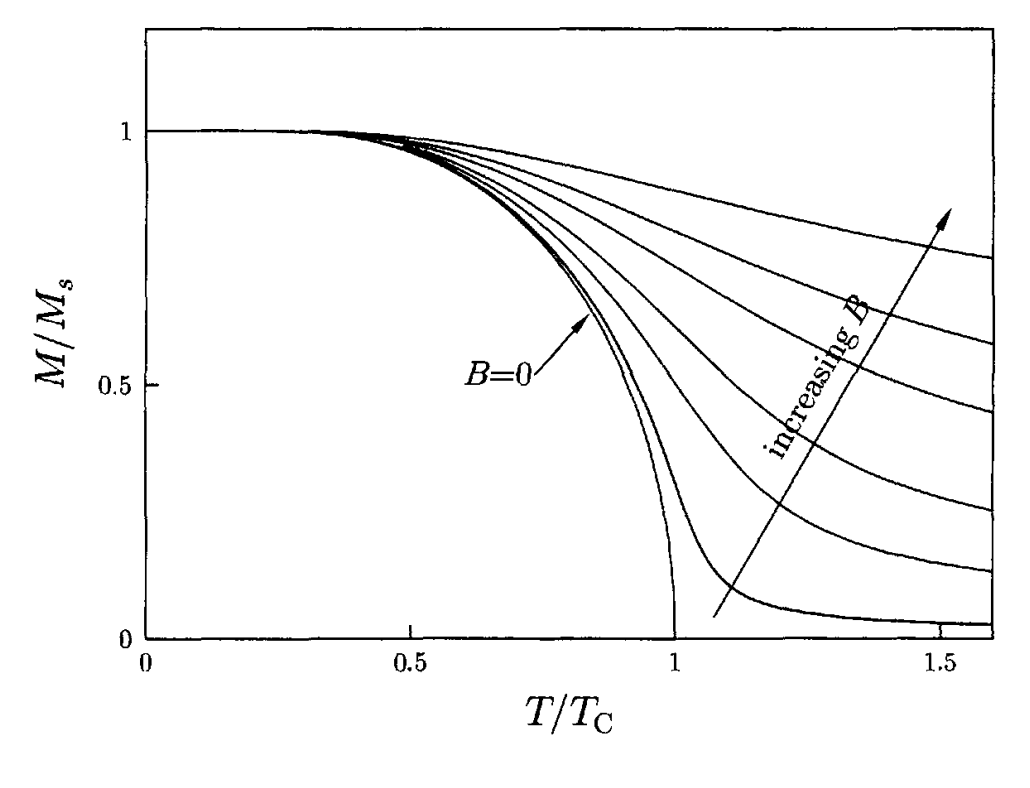
\includegraphics[width=.7\linewidth]{img/Ordnungsparam_Ext_Feld.png}
    \end{center}
    \refimgsourcebook{Magnetism In Condensed Matter (Oxford Master Series In Physics)}{Stephen Blundell}{978-0198505914}{90}
\end{fquestion}

% \begin{question}{Wie können wir die Symmetrie des Systems darstellen und die spontane Symmetriebrechung richtig beschreiben? }
%     Im ungebrochenen Zustand Parabelpotential gemalt (zuerst 2D, dann aber auch 3D erklärt), dann Übergang zum Doppelmuldenpotential erklärt als die Symmetriebrechung, gezeigt, wo sich im Potential der Grundzustand befindet und wie dieser sich ändert
% \end{question}

\begin{fquestion}{Was ist das Coleman-Theorem?}
    Das Coleman-Theorem dient zur Klassifizierung von Symmetriebrechungen.

    Gegeben sei ein quantenmechanisches System mit einer Lagrangedichte $\mathcal{L}$ und einem Zustand minimaler Energie, dem Vakuumzustand.
    Wirkt eine definierte Symmetrietransformation $U$ auf die Lagrangedichte $\mathcal{L}$ oder den Vakuumzustand, treten folgende Fälle auf:
    \begin{enumerate}
        \item Vakuumzustand und $\mathcal{L}$ sind invariant $\implies$ Exakte Symmetrie
        \item Vakuumzustand ist nicht invariant und
        \begin{enumerate}
            \item  $\mathcal{L}$ ist nicht invariant $\implies$ Explizite Symmetriebrechung
            \item $\mathcal{L}$ ist invariant  $\implies$ Spontane Symmetriebrechung
        \end{enumerate}
    \end{enumerate}
\end{fquestion}

\begin{fquestion}{Was ist das Goldstone-Theorem?}
    Die spontane Brechung globaler, kontinuierlicher Symmetrien hat zur Folge, dass zu jedem gebrochenen Generator der Symmetriegruppe ein masseloses skalares Teilchen entsteht.
    Vorstellen kann man sich dies als Anregung in Richtung der Symmetrie, für die eine zur Null fallende Dispersionsrelation gelten muss.
    Das entsprechende Quasiteilchen heißt Nambu-Goldstone-Boson, oder auch Goldstone-Boson.
\end{fquestion}

\subsection{Landau-Theorie}

\begin{fquestion}{Können wir Symmetriebrechung mathematisch beschreiben? }
    Ja, wir zum Beispiel mit der Landau-Theorie. 
    Dafür entwickeln wir das chemische Potential $F(T, \eta)$ in kleinen Ordnungsparametern (also nahe dem Phasenübergang):
    \[F(T, \eta) = F_0 + a(T) \eta^2 + \frac{b(T)}{2} \eta^4 + \mathcal{O}(\eta^6).\]
    Wir vernachlässigen die ungeraden Potenzen unter der Annahme, dass das System unter der Parität $\eta \rightarrow -\eta$ symmetrisch ist; natürlich muss diese Annahme nicht zwingend gelten.
    
    Aus $\partial F / \partial \eta = 0$ als angenommenen Zustand erhalten wir
    \[\eta^2 = - \frac{a(T)}{b(T)}.\]
    Außerdem fordern wir, dass wir uns in einem Potentialminimum befinden und damit $\partial^2 F / \partial^2 \eta = 2 a(T) + 6 b(T) \eta^2 > 0$.
    Hiermit folgt dass $a(T)$ bei $T=T_C$ einen Vorzeichenwechsel hat und die Näherung $a(T) = A (T - T_C)$ sinnvoll ist, $b(T) = B$ wird als konstant angenommen.
\end{fquestion}

\begin{fquestion}{Wieso ist der Parameter $a(T) < 0$ für $T < T_C$? }
    Damit sowohl Ordnungsparameter und zweite Ableitung der freien Energie als auch bspw. Entropie $S = \partial F / \partial T = S_0 - a Q^2$ und spezifische Wärmekapazität $C_p = T (\partial S / \partial T) = C_{p 0} + a^2 T_C/2 B$ (in der Hochtemperaturphase) sinnvoll positiv definiert sind.
\end{fquestion}

\begin{fquestion}{Welche Phasen gibt es in der Landautheorie?}
    \begin{minipage}{\linewidth}
        \begin{table}[H]
            \centering
            \begin{tabular}{|c|c|c|l|}
                \hline
                \textbf{Ordnungspar.} & \textbf{Koeffizienten} & \textbf{Temperatur} & \textbf{Phase} \\
                \hline
                $Q = 0$ & $A > 0$ & $T > T_C$ & Hochtemperaturphase \\
                \hline
                $Q = 0$ & $A = 0$ & $T = T_C$ & Phasenübergangspunkt \\
                \hline
                $Q^2 = -\frac{A}{B}$ & $A < 0, B > 0$ & $T < T_C$ & Tieftemperaturphase \\
                \hline
            \end{tabular}
        \end{table}
    \end{minipage}
\end{fquestion}

\begin{fquestion}{Wie kann man Phasenübergänge erster Ordnung in der Landau-Theorie beschreiben?}
    Wir führen zusätzlich einen Term $C \eta^6$ ein und können damit eine dreibäuchige freie Energie modellieren.
\end{fquestion}

\begin{fquestion}{Wie modelliert eine explizite Symmetrieänderung in der Landau-Theorie?}
    Durch einen zusätzlichen Term $h \eta$ linear im Ordnungsparameter.
\end{fquestion}




\subsection{Ferromagnetismus}

% Wichtig zu wissen ist die Curie-Temperatur $T_C = ?$ und dass die Magnetisierung als Ordnungsparameter fungiert.

\begin{fquestion}{Wie ist das mit der spontanen Symmetriebrechung, wenn ein äußeres Feld angelegt wird? }
    Sie tritt dann gar nicht auf, weil die Symmetrie schon explizit gebrochen wurde.
\end{fquestion}

% \begin{question}{Wie bekommt man einen Phasenübergang erster Ordnung?}
%     Term 6. Ordnung einführen 
% \end{question}

\begin{fquestion}{Was passiert wenn man die Symmetrie explizit bricht durch externes Magnetfeld?}
    Bei Landau Theorie durch Hinzufügen eines linearen Terms beschrieben. 
    
    Es findet kein Phasenübergang mehr statt. 
    
    Die Magnetisierung geht nicht auf Null runter sondern nähert sich nur mit 1/T an.
    
    Bei positiver Suszeptibilität, Paramagnet, wird das äußere Magnetfeld verstärkt. Bei negativer Suszeptibilität, Diamagnet, ist es umgekehrt. 
\end{fquestion}

% \begin{question}{Wie sieht die Magnetisierung bei endlichem Feld aus?}
%     bei hohen Feldern exponentiell unterdrückt
% \end{question}

\begin{fquestion}{Was haben ferromagnetische und chirale Symmetriebrechung gemeinsam?}
positive Rückkopplung, beispielsweise wird eine endliche Magnetisierung bis zur Sättigung verstärkt, dadurch, dass sich die Magnetisierung selbst beeinflusst. 
\end{fquestion}

\begin{fquestion}{Was gibt es für Anregungen im Ferromagneten?}
    Die Anregungen heißen Spinwellen, ihre Quasiteilchen heißen Magnonen.
\end{fquestion}

% \begin{question}{Sie hatten doch erwähnt, dass das auch von der Temperatur abhängig ist, wo steckt denn die T-Abhängigkeit? }
%     Im $a$-Faktor, s.d. $a=a_0(T-T_C)$
% \end{question}

% \begin{question}{Wie sieht dann denn die Energie für $T>Tc$ und $T<Tc$, Mexican-Hat in 2D für TTc nicht auf Null) ??? }
% \end{question}

\begin{fquestion}{Kein Knick mehr, was hat man an dem Knick denn erkannt?  }
    Phasenübergang 2. Ordnung ist, also eine Unstetigkeit in der ersten Ableitung. 
\end{fquestion}

% \begin{question}{Und was bedeutet das dann für die explizite Symmetriebrechung?}
%     Da hier kein Knick ist, ist es auch kein Phasenübergang mehr
% \end{question}

% \subsection{Ordnungsparameter und Brechungsparameter}

% \begin{question}{Wie ändert sich der Verlauf bei Existenz einer äußeren Feldes?}
%     An der kritischen Temperatur ist kein Knick, sondern ein abklingender Verlauf
% \end{question}

% \begin{question}{Wie ändert sich der Verlauf mit steigender äußerer Feldstärke?}
%     Der Bereich, in dem der Graph abfällt, verschiebt sich hin zu höheren Temperaturen
% \end{question}

% \begin{question}{Sind Symmetriebrechung und Phasenübergänge equivalent?}
%     Nein, Symmetriebrechung impliziert Phasenübergang, die Umkehrung gilt aber nicht
% \end{question}


\subsection{Higgs-Mechanismus}

Wichtig zu wissen sind die Lagrangedichte, Potential und Temperaturabhängigkeit.

\begin{fquestion}{Wie ist die Lagrangedichte des Higgsfeldes?}
    Es ist 
    $$\mathcal{L}(\phi) = (\partial_\sigma \phi)^\dagger (\partial^\sigma \phi) + \mu^2 \phi^\dagger \phi - \lambda (\phi^\dagger \phi)^2$$
    die Lagrangedichte des Higgsfeldes.
    Wir identifizieren das Potential
    $$\mathcal{V}(\phi) = -\mu^2 \phi^\dagger \phi + \lambda (\phi^\dagger \phi)^2,$$
    wobei $\mu = \SI{88.45}{GeV/c^2}$ eine Masse und $\lambda = 0.12907$ einheitenlos sind.
\end{fquestion}

\begin{fquestion}{Wie kommt es hier durch spontane Symmetriebrechung zum Massengewinn?}
    Wir betrachten als Modell das skalare Potential 
    $$V(\varphi) = -\mu^2 \varphi^2 + \lambda \varphi^4,$$
    welches sein Minimum bei dem sogenannten Vakuumerwartungswert
    $$\varphi_0 \equiv v = \pm \sqrt{\frac{\mu^2}{2\lambda}}$$
    hat.
    
    Wir entwickeln das ``Feld'' um den Grundzustand mit $\varphi \equiv v + H$ und erhalten
    $$V'(\varphi = v + H) = -\lambda v^4 + 4 \lambda v H^3 + 2 \mu^2 H^2 + \lambda H^4 = V_0 + 2 \mu^2 H^2 + \mathcal{O}(H^3),$$
    wobei das Higgsteilchen eine Masse $\frac{1}{2} m_H^2 = 2 \mu^2$ hat.
    Analog zum Klein-Gordon Feld beschreiben die $\mathcal{O}(H^3)$-Terme Wechselwirkung.
    
    In der komplexen Feldtheorie treten hierbei zwei Felder $h$ und $\chi$ auf, die Lagrangedichte lautet dann
    $$\mathcal{L}_{\mathrm{Higgs}}'(h, \chi) = \frac{1}{2} \partial_\sigma h \partial^\sigma h - \mu^2 h^2 + \frac{1}{2} \partial_\sigma \chi \partial^\sigma \chi + \mathrm{Wechselwirkungen}$$
    wobei das Higgsteilchen die Mase $m_hj = \sqrt{2} \mu$ und das $\chi$-Feld ein masseloses Nabu-Goldstone-Boson ist.
    
    Koppelt nun das Higgsfeld über
    $$\partial^\sigma \rightarrow D^\sigma = \partial^\sigma - i g A^\sigma$$
    an das Eichfeld $A^\sigma$ entsteht in der Lagrangedichte ein Term
    $$\mathcal{L}(A, h, \chi) = \frac{g^2 v^2}{2} A_\sigma A^\sigma + \ldots,$$
    der als Massenterm für das Eichfeld $A^\sigma$ interpretiert werden kann.
    
    Technisch muss hier noch das Eichfeld $\chi$ weggefressen werden, am Ende kommt man darauf dass $A^\sigma$ eine masselose Komponente und drei massive Komponenten hat.
\end{fquestion}

\begin{fquestion}{Wo tritt Massengewinn durch Symmetriebrechung auf?}
    Ein Massengewinn durch Symmetriebrechung tritt durch den Anderson-Higgs-Mechanismus bei der Supraleitung und beim Higgsfeld in der Teilchenphysik auf.
    
    Der Massengewinn durch die Symmetriebrechung des Higgsfeldes tritt bei allen an das Higgsfeld koppelnden Teilchen, also Quarks, $W$- und $Z$-Bosonen, sowie den geladenen Leptonen, auf und ist entsprechend für deren Masse verantwortlich.
    
    Genauso kann man beim Supraleiter die endliche Eindringtiefe der elektromagnetischen Felder als eine effektive Masse $m_A = \frac{2e}{\sqrt{m^\ast}} |\psi_0|$ der Photonen verstehen (quadratischer Term $\mathcal{L} = \dots + \frac{1}{2}m_A^2|\Vec{A}|^2$).
    % Massengewinn tritt auch durch bei der Symmetriebrechung der starken Wechselwirkung auf (SU$(2)_V \times $SU$(2)_A$ ??? ).
    % Hierbei tritt ein Phasenübergang von freien zu gebundenen Quarks auf.
    % Die Masse kommt dabei aus der Bindungsenergie, also den Gluonen und Seequarks.
    % bei den Konstituentenquarks der starken WW.
    % bei den endlichen (aber kleinen) ``nackten'' Quark-Massen.
    % bei der schwachen WW im Higgs-Mechanismus 
\end{fquestion}

% \begin{question}{Was passiert bei der schwachen Wechselwirkung?}
%     Lagrangedichte invariant, aber Grundzustand instabil, wenn Brechungsparameter bestimmten Wert überschreitet folgt dieser nicht mehr Symmetrie 
    
%     typisches $x^2$ und $x^4$ Potential zeichnen 
% \end{question}

\begin{fquestion}{Was ist das für eine Symmetrie die gebrochen wird?}
    Die schwache Eichsymmetrie.
\end{fquestion}

\begin{fquestion}{Warum beobachtet man die schwache WW nicht?}
    Aufgrund der Masse der W- und Z-Bosonen hat die Wechselwirkung eine sehr kleine Reichweite von nur $R \equiv \frac{1}{m_{W,Z}}\approx \SI{2.5e-3}{fm}$ (siehe Yukawa-Potential).
    Daher gibt es keine schwachen Bindungszustände (zumindest sind keine bekannt).
\end{fquestion}

% \begin{question}{Metastabiler Zustand?}
%     Term 6. Ordnung in Landau Theorie (Taylorentwicklung, lässt höheren Ordnungen üblicherweise weg)
% \end{question}

% \begin{question}{Kinetischer Term?}
%     kin. Term der freien Energy des Ferromagneten ???
% \end{question}

\begin{fquestion}{Warum braucht man überhaupt das Higgs-Teilchen?}
    Bei der elektroschwachen Vereinigung kann sonst nicht erklärt werden, wieso das Photon masselos, die drei $W$- und $Z$-Bosonen aber sehr schwer sind.
\end{fquestion}

% \begin{question}{Wie bekommt man Masse, Anregungen?}
%     massive und masselose Anregungen zeichnen ???
%     diese sind Higgs-Boson und Nambu-Goldstone-Bosonen die zu den W/Z-Bosonen beitragen
% \end{question}

% \begin{question}{Wieso haben W, Z Masse wenn NG-Bosonen masselos?}
%     wegen Higgsfeld mit Vakuumerwartungswert ungleich Null
% \end{question}

\begin{fquestion}{Was passiert bei höheren Temperaturen?}
    Bei höheren Temperaturen ($T \gtrsim \SI{1e15}{K}$, etwa beim Beginn des Universums) ist $-\mu^2 > 0$, also findet keine spontane Symmetriebrechung statt und die Austauschteilchen sind masselos.
\end{fquestion}

\begin{fquestion}{Welcher Term hängt dann im Potential von der Temperatur ab?}
    Wie bei anderen Theorien postuliert man $\mu^2(T) = \alpha (T_c-T)$.
\end{fquestion}

% \begin{question}{Grundzustand?}
%     Diagramm (analog M(T) für Ferromagnetismus), hier Vakuumerwartunswert anstatt Magnetisierung
% \end{question}

% \begin{question}{Worin äußert sich Higgs-Symmetriebrechung? }
%     Kosmischer Supraleiter, endliche Reichweite der WW-Bosonen und somit Masse
%     Analogie Higgs-Mechanismus zur Londonschen Eindringtiefe und Reichweite
% \end{question}

\begin{fquestion}{Was sind die Analogien des Higgs-Mechanismus zum Supraleiter?}
    Der Higgsmechanismus hat viele Analogien bei den Supraleitern, vor allem beim Meißner-Ochsenfeld-Effekt: Magnetfelder breiten sich in der supraleitenden Phase nur bis zur Londonschen Eindringtiefe $\lambda$ aus, was man mit einem massebehafteten Austauschteilchen assoziiert.
    Analog ist die kurze Reichweite der $W$- und $Z$- Bosonen mit ihrer Masse verbunden ($\lambda_W = \frac{1}{m_W} \approx \SI{2.5e-3}{fm}$).
    
    Die Koherenzlänge ist $\xi_W = \frac{1}{m_H} \approx \SI{1.6e-3}{fm}$.
    Beim Supraleiter hängt sie mit dem Durchmesser von Flussschläuchen über $d=2\xi$ zusammen.
    Analog dazu wären sogenannte (hypothetische) ``cosmic strings''.
\end{fquestion}

\begin{fquestion}{Wie vermisst man den Higgs Mechanismus, wo doch $T_c$ so hoch ist?}
    Es ist $T_c \approx \SI{e15}{K} \approx 10^8\, T_{\mathrm{Sonnenkern}}$. 
    Man kann zwar den Phasenübergang nicht beobachten misst dafür aber, wie das Higgs-Boson an andere Elementarteilchen (etwa die $W$-Bosonen) koppelt.
\end{fquestion}

\subsection{Supraleitung}

Zum Einarbeiten in die Supraleitung kann das Kapitel 6 - Supraleitung im 6. Band zur Festkörperphysik des Bergmann, Schäfer empfohlen werden.

\begin{fquestion}{Was ist der Meißner-Effekt?}
    Der Meißner-Effekt beschreibt, dass Typ I Supraleiter Magnetfelder vollständig aus ihrem Inneren verdrängen. 
\end{fquestion}

\begin{fquestion}{Was ist die Ginzburg-Landau-Theorie?}
    Sie ist eine Erweiterung der Landau-Theorie, in welcher der Ordnungsparameter ortsabhängig sein darf.
    Dementsprechend gibt es dann in Lagrangedichte oder freier Energie üblicherweise einen ``kinetischen Term'', der durch das Quadrat einer ersten Ableitung gegeben ist.
    
    Im Kontext der Supraleitung gibt die Theorie eine makroskopische, phänomenologische Beschreibung. 
    Sie ist nur für Supraleiter 1. Art gültig, weil sie die Flussliniengitter in der Shubnikov-Phase nicht beschreiben kann.
\end{fquestion}

\begin{fquestion}{Was beschreibt das kritische Feld $B_c$ in der Ginzburg-Landau-Theorie?}
    Bei der kritischen Feldstärke $B_c = \sqrt{\mu_0 \frac{a(T)^2}{b(T)}}$ findet ein Phasenübergang im Supraleiter statt; übersteigt das äußere Feld diesen Wert bricht die supraleitende Eigenschaft zusammen und der Supraleiter bildet ein intrinsisches Magnetfeld aus. 
    Typischerweise ist $B_c = \SI{0.08}{\tesla}$ (Pb) oder $B_c = \SI{0.01}{\tesla}$ (Al).
\end{fquestion}

\begin{fquestion}{Was ist die Londonsche-Eindringtiefe $\lambda$?}
    Sie gibt an, wie tief das Magnetfeld in einen Körper eindringen kann (ähnlich einem exponentiellen Zerfall).
    Sie ist durch  
    \[\lambda_L = \sqrt{\frac{m_e}{\mu_0 n q^2}} \approx 20 \ldots 200\, \si{\nano \metre}\]
    gegeben, wobei $q = 2 e$ wegen der Cooperpaare ist.
\end{fquestion}

\begin{fquestion}{Was ist die Ginzburg-Landau Kohärenzlänge $\xi$?}
    Die Kohärenzlänge bestimmt, wie stark die Wellenfunktion im Supraleiter variiert, ist also ein Maß der thermodynamischen Fluktuationen in der supraleitenden Phase.
    Es ist 
    \[\xi = \sqrt{\frac{\hbar^2}{2 m^\star a(T)}} = 1 \ldots 1000\, \si{\nano\metre}.\]
\end{fquestion}

\begin{fquestion} {Was ist der Ginzburg-Landau-Parameter $\kappa$?}
    Das Verhältnis von Eindringtiefe und Kohärenzlänge \(\kappa = \frac{\lambda}{\xi}\).
\end{fquestion}

% \begin{question}{Wie funktioniert die energetische Betrachtung?}
%     Freie Energie aufschreiben, zwei konkurrierende Terme (Supraleitendes Potential und Magnetfeld) ???
% \end{question}

\begin{fquestion}{Was ist das Besondere an der supraleitenden Phase? }
    In der supraleitenden Phase ist der Körper ein idealer Diamagnet (stößt äußeres Magnetfeld ab) und idealer Leiter.
\end{fquestion}

\begin{figure}[!ht]
    \centering
    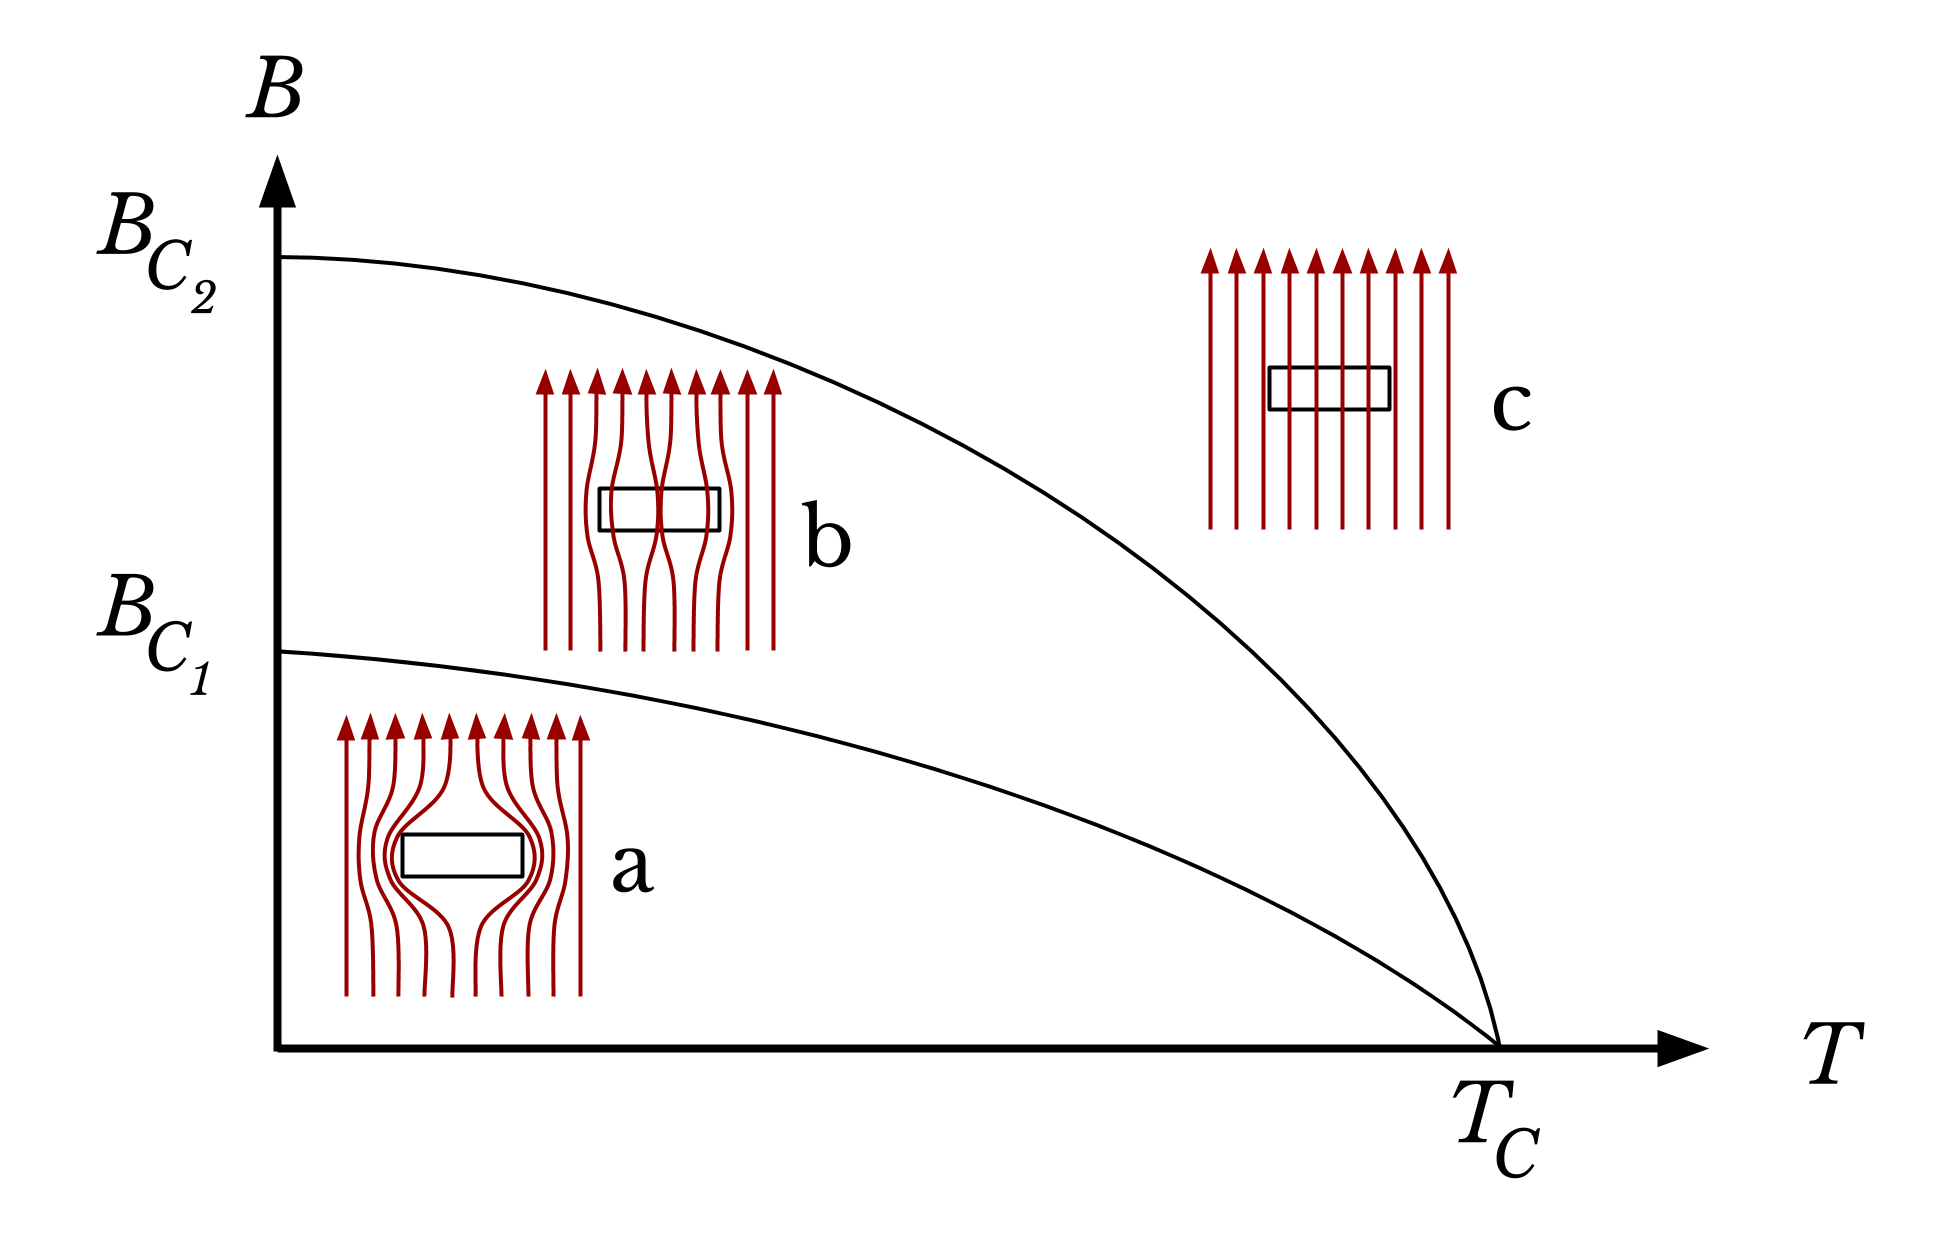
\includegraphics[width=\linewidth]{img/Superconductor_type2_phase_diagram.png}
    \caption{Phasendiagramm eines Supraleiters 2. Art.
    Die dargestellten Phasen sind (a) supraleitend, (b) Misch- oder Shubnikovphase und (c) normalleitend.
    In einem Supraleiter 1. Art existiert (b) nicht, dementsprechend gibt es dort auch nur ein kritisches Magnetfeld $B_c$.
    \refimgsource{Wikimedia}{https://commons.wikimedia.org/wiki/File:Superconductor\_interactions\_with\_magnetic\_field.png}{23.02.2022}{public domain}}
    \label{fig:superconductor type 2 phase diagram}
\end{figure}

\begin{fquestion}{Wie unterscheidet man Supraleiter?}
    Man unterscheidet zwischen Typ I ($\kappa < \frac{1}{\sqrt{2}}$, $\xi$ groß und $\lambda$ klein) und Typ II ($\kappa > \frac{1}{\sqrt{2}}$, $\xi$ klein und $\lambda$ groß) Supraleitern.
    
    Bei Typ II Supraleitern findet der Phasenübergang von der Meißner-Phase (Supraleitenden Phase) zur normalleitenden Phase über eine Mischphase (Shubnikov-Phase) statt. 
    In der Mischphase bilden sich Flussschläuche aus.
    
    Bei Typ I Supraleitern ist der Phasenübergang abrupt, siehe auch \autoref{fig:superconductor type 2 phase diagram}.
    
    Die zwei Arten unterscheiden sich auch im $B-B_a$-Diagramm (Inneres-Äußeres-Magnetfeld).
    Der Typ I Supraleiter entwickelt bei $B_a = B_c$ sprunghaft ein inneres Magnetfeld, der Typ II Supraleiter beginnt ab $B_a = B_{c1}$ dieses stetig auszubilden.
    
    \begin{center}
        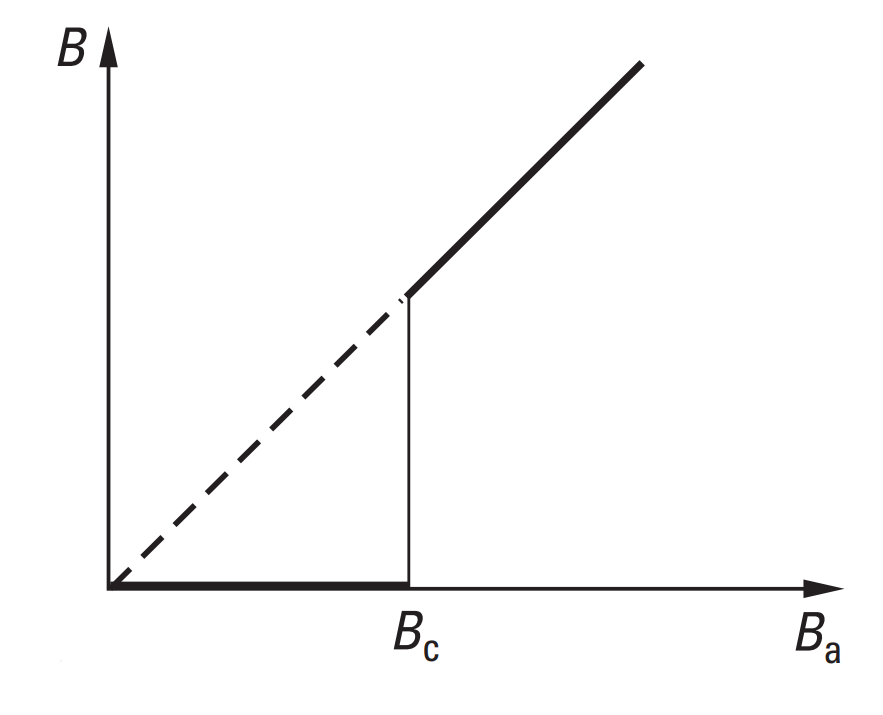
\includegraphics[width=0.4\linewidth]{img/Supraleiter_typ1.png}
        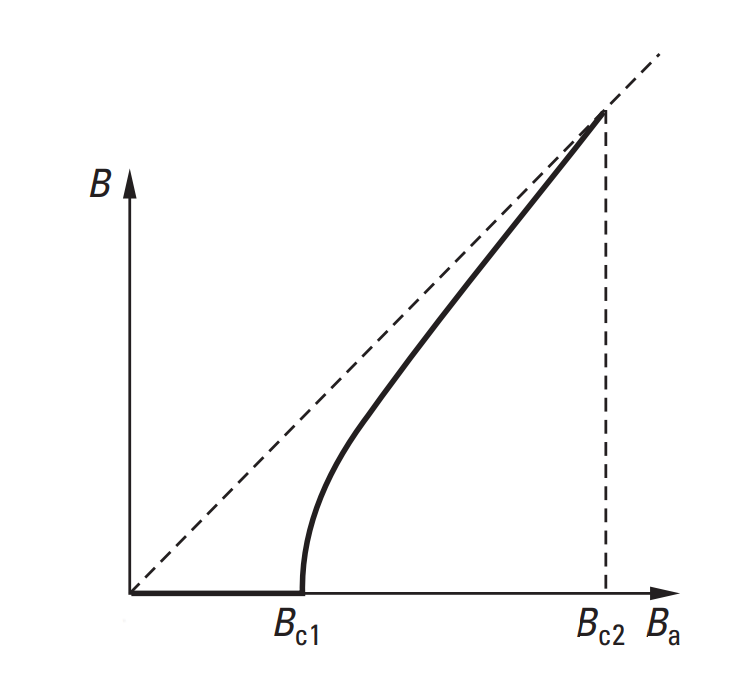
\includegraphics[width=0.4\linewidth]{img/Supraleiter_typ2.png}
    \end{center}
    \refimgsourcebook{Festkörper (Experimentalphysik, Band 6)}{Bergmann, Schäfer}{3110174855}{489f}
\end{fquestion}

\begin{figure}[!ht]
    \centering
    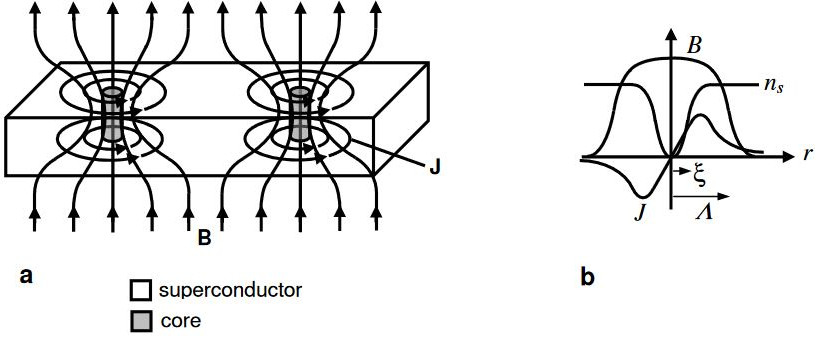
\includegraphics[width=.8\linewidth]{img/SuperconductorVortexStructure.jpg}
    \caption{Schematische Darstellung eines Flussschlauches. 
    In (a) ist das Eindringen des magnetischen Flusses über Wirbel dargestellt. 
    In (b) ist der Querschnitt eines Flussschlauches mit $B$-Feld, Kohärenzlänge $\xi$, Eindringtiefe $\Lambda$ ($\lambda$), sowie Teilchenzahl im supraleitenden Zustand $n_s$ und supraleitende Stromdichte $J$ dargestellt.
    \refimgsource{nLab}{https://ncatlab.org/nlab/files/SuperconductorVortexStructure.jpg}{17.02.2022}{Keine}}
    \label{fig:flussschlaeuche}
\end{figure}

\begin{fquestion}{Was sind Flussschläuche?}
    Flussschläuche sind die Erklärung dafür, dass bei Supraleitern 2. Art der Meißner-Ochsenfeld Effekt ab einer kritischen Temperatur bzw. einer kritischen Feldstärke nicht mehr erfüllt ist, ohne die supraleitende Eigenschaft zu verlieren.
    
    Flussschläuche sind Wirbel (Defekte) im Supraleiter, deren Inneres nicht supraleitend ist. 
    In ihrem Inneren herrscht eine Flussdichte von $\Phi_0 = \frac{h}{2e}$. 
    Eine schematische Skizze ist in \autoref{fig:flussschlaeuche} dargestellt.
\end{fquestion}

\begin{fquestion}{Was sind Beispiele für Supraleiter?}
    In der folgenden Tabelle sind verschiedene Supraleiter aufgeführt:
    \begin{center}
        \begin{tabular}{|l|lllll|}
            \hline
            Material & $T_C\, /\, \si{\kelvin}$ & $\xi\, /\, \si{\nano\metre}$ & $\lambda\, /\, \si{\nano\metre}$ & $\kappa$ &  \\
            \hline
            Al & $1.18$ & $1600$ & $50$ & $0.03$ & Typ I \\
            Pb & $7.19$ & $83$ & $39$ & $0.47$ & Typ I \\
            \hline
            Nb & $9.25$ & $40$ & $44$ & $1.1$ & Grenzfall\\
            \hline
            $\text{Nb}_3\text{Sn}$ & $18.2$ & $3.6$ & $124$ & $34$ & Typ II \\
            $\text{YBa}_2\text{Cu}_3\text{O}_{7 - \delta}$ & $90$ & $(1.5)$ & $(130)$ & $(87)$ & Typ II \\
            \hline
        \end{tabular}
    \end{center}
\end{fquestion}

% \begin{question}{Was ist ein Typ 2 Supraleiter}
%     Es kommt zu Flussschläuchen, da weder Verlust durch Verdrängung des Magnetfeldes, noch durch Unterbrechung der SL-Phase (FS sind energetisch günstiger)
% \end{question}

\begin{fquestion}{Wie kann man einen verschwindenden elektrischen Widerstand $R = 0$ messen?}
    Mit klassischen Widerstandsbrücken erhält man eine obere Schranke $R / R_n < 10^{-4}$, wobei $R$ der Widerstand in der supraleitenden und $R_n$ der in der normalleitenden Phase sind.
    Für genauere Messung benötigt man Induktionsexperimente: Etwa durch einen Stabmagneten wird in einer supraleitenden Spule ein Strom induziert, der entsprechend $ I \propto \exp \left(-R/L t\right)$ abklingt. 
    Wenn $R= 0$ ist die Abklingdauer unendlich und tatsächlich ist dadurch $R / R_n < 10^{-14}$ (über das magnetische Moment $m = I A$) messbar.
\end{fquestion}

\begin{fquestion}{Was ist die BCS-(Bardeen-Cooper-Schrieffer)-Theorie? }
    Die BCS-Theorie kann Typ I Supraleiter erklären. 
    In der BCS-Theorie werden Elektronen durch eine anziehende Wechselwirkung miteinander korreliert und bilden Cooper-Paare mit ganzzahligem Spin, unterliegen also der Bose-Einstein-Statistik. 
    
    Formell entstehen sie durch die Wechselwirkung von zwei Elektronen auf Fermi-Niveau (Streuung  an einem virtuellen Phonon), was zu einer Energieabsenkung 
    \[E \approx 2 E_F - 2 \hbar \omega_D e^{-4 / D(E_F) V_0} := 2 E_F - 2 \Delta\]
    führt.
    Für die Cooper-Paare ist es also sinnvoll in einen Grundzustand unterhalb der Fermi-Energie zu kondensieren (ist nicht das selbe wie ein Bose-Einstein-Kondensat).

    Siehe \url{https://www.thphys.uni-heidelberg.de/~wolschin/qms1920_11s.pdf}.
\end{fquestion}

\begin{fquestion}{Wie entstehen Cooper-Paare heuristisch?}
    Im Kristall entstehen Cooper-Paare durch Interaktion mit dem Gitter.
    Bewegt sich ein Elektron an Gitterplätzen vorbei, bewegen sich die positiv geladenen Atomkerne leicht in Richtung des Elektrons, wodurch eine positive Nettoladung entsteht.
    Ein Elektron entgegengesetzten Spins und Impulses interagiert mit dieser Ladung und die Elektronen werden korreliert.
\end{fquestion}

\begin{fquestion}{Wie erklären Cooper-Paare Supraleiter?}
    Der Widerstand wird durch inelastische Streuprozesse verursacht.
    Damit ein Cooper-Paar inelastisch streuen kann, muss die Energielücke $2\Delta$ überwunden werden, was bei niedrigen Temperaturen nicht möglich ist (die phänomenologische Erklärung ist hier, dass die Cooper-Paare mit $\approx \SI{100}{\nano\metre}$ weit auseinander sind und die Gitterfehler nicht spüren).
    Durch das Kondensat müssten elastische Stöße auf alle Cooper-Paare gleichzeitig wirken, wodurch die Streuung (beliebig unwahrscheinlich) nicht möglich ist.
    
    Erreicht der Strom im Leiter eine kritische Stromdichte $j_C = -e n \Delta / \hbar k_F$, können jene inelastischen Streuprozesse stattfinden und der Supraleiter bricht zusammen (das kritische Magnetfeld $B_C$ kann genau solche Ströme induzieren). 
\end{fquestion}

\begin{fquestion}{Was sind Cooper-Paare?}
    % zwei Elektronen werden durch Phononen aneinander gebunden (Ladung 2e)
    % 
    % entgegengesetzter Impuls (gleicher Betrag) und entgegengesetzter Spin (Gesamtspin S=0)
    % Erhöht oder verringert sich die Energie bei Paarbildung?
    % 
    % Cooper-Paare sind energetisch günstiger, (Zeichnung Bandlücke ??? )
    % 
    Cooper Paare sind zwei Elektronen die durch einen anziehende Wechselwirkung aneinander gebunden sind.
    Die Elektronen der Cooper-Paare tragen \textbf{entgegengesetzten Impuls}, weil dort die Wechselwirkung den größten Phasenraum (am Fermi-Rand) abdeckt und diese Paarung entsprechend am wahrscheinlichsten ist.
    Da der Ort symmetrisch gewählt wird, muss der \textbf{Spin antisymmetrisch} (entgegengesetzt sein).
    
    Die Dispersionsrelation eines Cooper-Paares ist 
    \[ E_k = \sqrt{\epsilon_k^2 + \Delta^2}\]
    wobei $\epsilon_k$ die kinetische Energie (wahlweise abzüglich des chemischen Potentials $\epsilon_k' := \epsilon_k - \mu$) der Elektronen und $\Delta$ die Bandlücke des Supraleiters ist.
    Die Cooper-Paarbildung ist entsprechend energetisch günstiger als die Bevölkerung des Fermi-Sees.
    
    Die Cooper-Paar-Kondensation führt zu einer Änderung der Zustandsdichte im Vergleich zum freien Elektronengas mit entsprechender Bandlücke:
    \begin{center}
        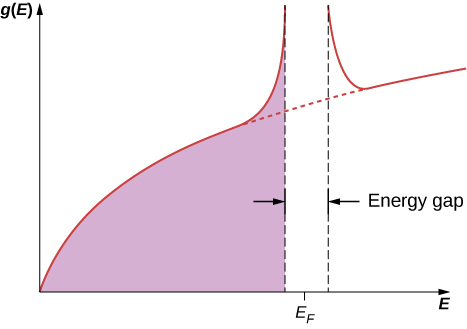
\includegraphics[width=0.5\linewidth]{img/CNX_UPhysics_42_08_EnergyGap-1.jpg}
    \end{center}
    \refimgsource{University Physics Volume 3}{https://opentextbc.ca/universityphysicsv3openstax/chapter/superconductivity/}{30.01.2022}{Creative Commons Attribution 4.0 International License}
    % 
    % Der Streuprozess, der zur Bildung von Cooper-Paaren führt ist nur durch zusätzliche kinetische Energie (etwa eine Temperatur $T \neq 0$) möglich.
    % 
    % Bindung im meV Bereich (-> thermische Energie 25 meV!)
    % Wie kann man Cooper-Paar-Bildung anschaulich erklären? 
    % 
    % Zeichnung Auslenkung des Ionengitters durch Elektron
    % Steht die Paarbildung nicht im Widerspruch zur 1. Hundschen Regel?
    % 
    % Muss wegen hohem mittleren Abstand der Elektronen nicht berücksichtigt werden
    % Wieso streuen Cooper-Paare nicht an Gitterfehlern?
    % 
    % Durchschnittlicher Abstand im Cooper-Paar ist 100 nm, also recht groß. 
    % 
    % Entweder zerbricht das Cooper-Paar an dem Gitterfehler (wenn die Energie groß genug ist) oder das Elektron streut nicht, da ansonsten gleichzeitig das Elektron 100 nm entfernt auch streuuen müsste (die Wahrscheinlichkeit quasi 0).
\end{fquestion}

\begin{fquestion}{Wie verhält sich die Wärmeleitung in der supraleitenden Phase?}
    Die Cooper-Paare tragen keine Entropie; kondensieren diese nimmt der elektronische Beitrag zur Wärmeleitung rapide ab.
    Kompensiert wird dieser Effekt durch das Ausfrieren der Gitterplätze, wodurch die Wärmeleitung im Allgemeinen steigt.
\end{fquestion}

% \begin{question}{Wie misst man, dass Phononen für die Cooper-Bindung verantwortlich sind?}
%     Der Effekt der Supraleitung ist streng mit dem Gitter verbunden, entsprechend kommen nur Phononen in Frage.    
% \end{question}

% \begin{question}{Wie misst man, dass Phononen für die Cooper-Bindung verantwortlich sind?}
%     Frequenz der Phononen ändern -> Änderung der WW ???
%     gleichen Supraleiter mit unterschiedlichen Isotopen messen -> ändert Atommassen -> ändert Frequenz -> ändert Bindung ???
% \end{question}


% \begin{question}{Welche zwei Längen sind für Supraleiter wichtig? Warum und wie erhält man diese?}
%     London'sche Eindringtiefe, Kohärenzlänge (Größenordnung ??? )
    
%     Unterscheidung von Typ I und Typ II Supraleitern (auch ??? ) anhand dieser Längen
% \end{question}

% \begin{question}{Wie kann man die Phononenanregung im Supraleitern untersuchen? }
%     Isotopeneffekt, Proportionalität der Schwingungsfrequenz zu k/m über das Hook'sche Gesetz und das Lösen der DGL des HO
% \end{question}


\begin{fquestion}{Warum ist die kritische Temperatur bei Supraleitern so klein?}
    Damit die Supraleitende Anregung messbar wird, müssen thermische Fluktuationen unter der durch die Phononanregung entstehenden Energielücke sein. 
    Entsprechend ist 
    \[T_C \propto \frac{1}{\sqrt{M}}\]
    wobei $M$ die Isotopmasse ist, entsprechend ist $T_C$ sehr klein. 
\end{fquestion}

\begin{fquestion}{Was ist der Zusammenhand zwischen der BCS- und der GLA-Theorie?}
    Der Ordnungsparameter der Ginzburg-Landau Theorie ist die Anzahl der Cooper-Paare in der BCS-Theorie.
\end{fquestion}

\begin{fquestion}{Was ist Josephson Tunneln?}
    Beim \textit{Josephson Tunneln} wird der Tunneleffekt zwischen zwei Supraleitern (getrennt durch Normalleiter oder Isolator) untersucht.
    Legt man an diese Josephson-Kontakte eine Spannung an, können die Cooper-Paar-Quasiteilchen durch die Barriere tunneln und ein Stromfluss entsteht.    
\end{fquestion}

\subsection{Deformierte Kerne}

% \begin{question}{Was sind die Ordnungs- und Brechparameter?}
%     Deformation (Ordnungsparameter) und Zahl der Valenznukleonen (Brechparameter)
% \end{question}

\begin{fquestion}{Wie kann man deformierte Kerne über Symmetriebrechung beschreiben?}
    Man betrachtet die Deformation als Ordnungsparameter und die Zahl der Valenznukleonen als Brechungsparameter im Landau-Zener-Modell.
\end{fquestion}

\subsection{Phasenübergänge}

\begin{fquestion}{Wie werden Phasenübergange charakterisiert?}
    Phasenübergänge werden nach Ehrenfest in jene $n$-ter Ordnung unterteilt.
    Dabei beschreibt $n-1$, die wie vielte Ableitung eines thermodynamischen Potentials beim Phasenübergang nicht stetig ist.
    Für $n=1$ spricht man von Phasenübergängen erster Ordnung, hier ist das Thermodynamische Potential selbst unstetig, bei $n>1$ spricht man von stetigen Phasenübergängen.
\end{fquestion}

\begin{fquestion}{Was haben Phasenübergänge 1. Klasse mit latenter Wärme zu tun?}
    Am Beispiel des schmelzenden Wassers kann man das erkennen: Hier muss man immerzu (Schmelz-)Wärme zuführen, ohne dass die Temperatur steigt. 
    Die erste Ableitung der freien Enthalpie $G$ nach $T$ (die Entropie $S$) ist entsprechend unstetig.
\end{fquestion}

\begin{figure}[!ht]
    \centering
%    \includesvg[scale=0.6]{img/Phasendiagramme.svg}
    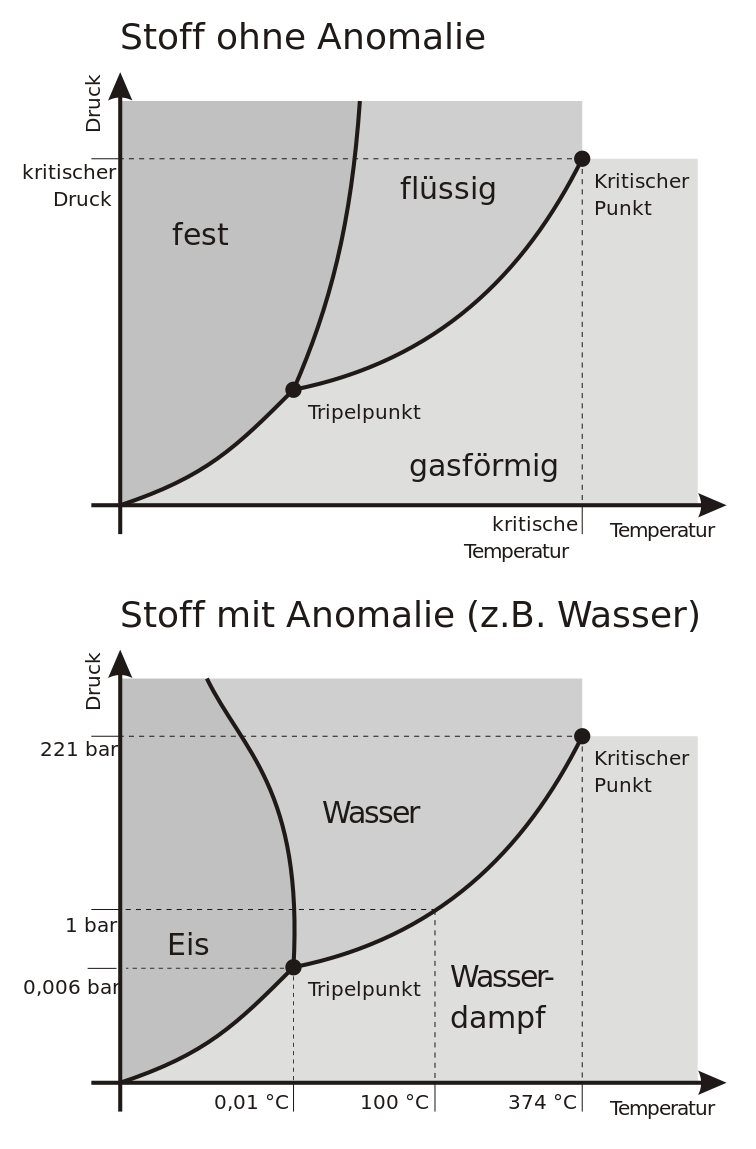
\includegraphics[width=0.6\linewidth]{img/Phasendiagramme.png}
    \caption{Phasendiagramme von Reinstoffen in der Druck-Temperatur-Ebene. Oben: ``normales'' Verhalten – die Schmelzdruckkurve zwischen fester und flüssiger Phase hat eine positive Steigung. Unten: Reinstoff mit Dichteanomalie wie etwa Wasser– die Schmelzdruckkurve zwischen fester und flüssiger Phase hat eine negative Steigung.   \refimgsource{Wikimedia}{https://commons.wikimedia.org/wiki/File:Phasendiagramme.svg}{18.01.2022}{public domain}}
\end{figure}


\cleardoublepage
\section{Zustandsmischungen}
\addcontentsline{qst}{section}{\thesection \hspace{.5em} Zustandsmischungen}
Beispiele und Anwendungen von Zustandsmischungen:
\begin{itemize}
    \item Ammoniak,
    \item Neutrinos,
    \item Neutrale Kaonen,
    \item Maser
\end{itemize}

\subsection{Ammoniak}

\begin{figure}[H]
    \centering
    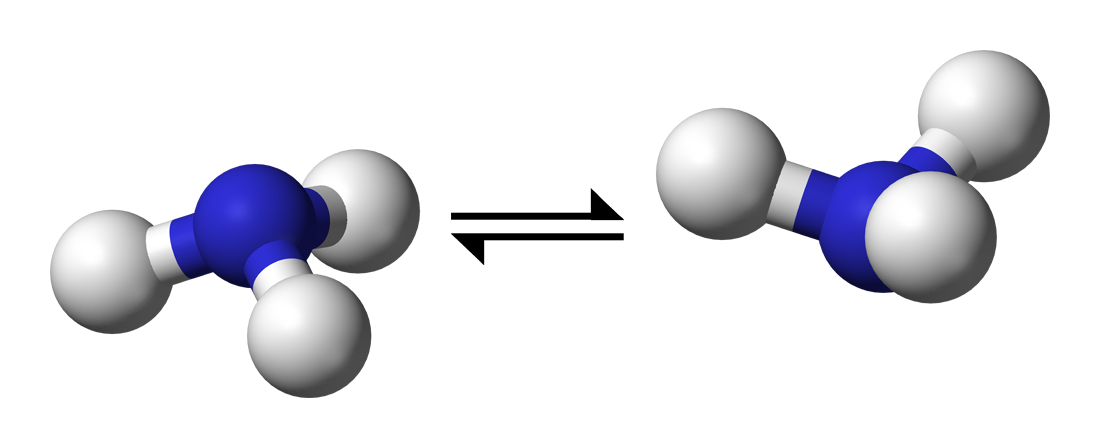
\includegraphics[scale=0.3]{img/Nitrogen-inversion-3D-balls (1).png}
    \caption{Stickstoff- (oder Schirm-) Inversion in Ammoniak. \refimgsource{Wikimedia}{https://commons.wikimedia.org/wiki/File:Nitrogen-inversion-3D-balls.png}{18.01.2022}{public domain}}
    \label{fig:my_label}
\end{figure}

\begin{fquestion}{Wie ist die Formel für gemischte Zustände mit den dazugehörigen Energien?}
    Die Formel für den gemischten Zustand ist hier
    \[\ket{\Psi(t)} = \sum_n c_n \ket{\psi_n} \e^{-\frac{\i}{\hbar} E_n t} = c_1 \ket{1} \e^{-\frac{\i}{\hbar} E_1 t} + c_2 \ket{2} \e^{-\frac{\i}{\hbar} E_2 t}\]
    wobei $\ket{1}$ und $\ket{2}$ jeweils die beiden Symmetriezustände (Stickstoff ober- oder unterhalb der Wasserstoffebene beschreiben).
    Der Hamiltonian des Systems ist allgemein
    \[H = \begin{pmatrix} E_0 & -A \\ -A & E_0 \end{pmatrix}\]
    mit der Grundenergie der beiden Symmetriezustände $E_0$ und der Energie aus dem Überlappintegral $A = \braket{1 | H}{2}$.
    Die Eigenenergien sind
    \[E_\pm = E_0 \pm A.\]
\end{fquestion}

% \begin{question}{Zeichnung gekreuzte Zustände ohne E-Feld? (Zeichnung Amoniak Molekül)}
%     Mittelpunkt der linearen Kreuzung ???
%     Wo liegen sie mit Feld? 
%     auf y-Achse im Minimum der ALC ???
%     Skizze mit den Zustandsenergien als Hyperbeln ???
%     Landau-Zehner-Wahrscheinlichkeit ???
% \end{question}

\begin{fquestion}{Welchen Einfluss hat das Elektrische Feld?}
    Das elektrische Feld führt aufgrund des Dipolmomentes $p$ in Symmetriezustände zu einer Unterscheidung beiden, wobei \(E_1 = E_0 + p \mathcal{E}\) und \(E_1 = E_0 - p \mathcal{E}\).
    Damit ändern sich die Eigenenergien zu
    \[E_\pm = E_0 \pm \sqrt{A^2 + p^2 \mathcal{E}^2}.\]
\end{fquestion}

\begin{fquestion}{Wieso spielt das elektrische Feld eine Rolle?}
    Das elektrische Feld ermöglicht ein kontrolliertes Anfahren des Level-Crossings (siehe Maser).
\end{fquestion}

\begin{figure}[H]
    \centering
    % \includesvg[scale=0.4]{img/Stern-Gerlach_experiment_svg.svg}
    \includegraphics[width=0.9\linewidth]{img/Stern-Gerlach_experiment_svg.png}
    \caption{Stern–Gerlach experiment: Silver atoms travelling through an inhomogeneous magnetic field, and being deflected up or down depending on their spin; (1) furnace, (2) beam of silver atoms, (3) inhomogeneous magnetic field, (4) classically expected result, (5) observed result. \refimgsource{Wikimedia}{https://commons.wikimedia.org/wiki/File:Stern-Gerlach_experiment_svg.svg}{18.01.2022}{Creative Commons Attribution-Share Alike 4.0 International}}
    \label{fig:zustandsmischung:stern-gerlach}
\end{figure}

\begin{fquestion}{Wie kann man die Mischung sichtbar machen?}
    Die Mischung kann mit einem Stern-Gerlach Apparat sichtbar gemacht werden, siehe \autoref{fig:zustandsmischung:stern-gerlach}. 
    Durch ein inhomogenes Feld quer zur Strahlachse erfolgt eine Auftrennung der Zustände.
    Durch ein langsames Absenken des Feldes, wird verhindert, dass die Zustände direkt wieder durch Tunneln mischen.
\end{fquestion}

\begin{fquestion}{Wie kann man das experimentell überprüfen?}
    Durch einen Maser.
    Für NH${}_3$ ist $\omega = \SI{24}{GHz}$.
\end{fquestion}

\begin{fquestion}{Wie ist der Mischungswinkel?}
    Es ist $\theta_m = \SI{45}{\degree}$.
\end{fquestion}

\subsection{Avoided Level Crossing (ALC)}

\begin{figure}[H]
    \centering
    \begin{tikzpicture}[scale=4,cap=round]
        
        \coordinate (A) at (0,0);
        \coordinate (B) at (1.5,1);
        \coordinate (C) at (0,1);
        \coordinate (D) at (1.5,0);
        \coordinate (M) at (0.75,0.5);
        
        \coordinate (CO) at (-0.25, -0.15);
        \coordinate (CT) at (-0.25, 1.25);
        \coordinate (CR) at (1.75, -0.15);
        \coordinate (CM) at (0.75, -0.15);
        
        \draw[color=blue, thick] (A) .. controls (M) ..  (D);
        \draw[color=blue, thick] (B) .. controls (M) ..  (C);
        \draw[dashed] (A) to (B);
        \draw[dashed] (C) to (D);
        
        \node[anchor=east] at (A) {$\ket{1}$};
        \node[anchor=west] at (B) {$\ket{1'}$};
        \node[anchor=east] at (C) {$\ket{2}$};
        \node[anchor=west] at (D) {$\ket{2'}$};
        
        
        \node[anchor=south,text=blue] at ($(M)+(0,0.2)$) {$\ket{\phi_2}$};
        \node[anchor=north,text=blue] at ($(M)-(0,0.2)$) {$\ket{\phi_1}$};
        
        \draw[color=black, -{Stealth[length=3mm,width=2mm]}] (CO) to (CT);
        \draw[color=black, -{Stealth[length=3mm,width=2mm]}] (CO) to (CR);
        
        \node[anchor=south] at (CT) {$V(z)$};
        \node[anchor=west] at (CR) {$z$};
        
        \draw[color=black] ($(CM)+(0,-0.025)$) to ($(CM)+(0,0.025)$);
        \node[anchor=north west] at (CM) {$z_c$};
        
    \end{tikzpicture}
    \caption{Skizze eines Avoided Crossing. Im Graph sind die Energien eines Systems in Abhängigkeit einen Parameters $z$ dargestellt. Die gestrichelte Linie entspricht dem diabatischen (schnellen) Übergang, bei dem ein Crossing der Eigenzustände $\ket{1}$ und $\ket{2}$ bei $z_c$ stattfindet, die durchgezogenen Linien entsprechen dem adiabatischen (langsamen) Übergang (den Eigenwerten $\ket{\phi_1}$ und $\ket{\phi_2}$ des Hamiltonians).}
\end{figure}

\begin{fquestion}{Was ist Avoided Level Crossing?}
    Von einem Avoided Level Crossing spricht man, wenn die Energieeigenwerte eines Systems von einem kontinuierlichen Parameter (etwa der Zeit $t$ oder einem äußeren Feld $\mathcal{E}$) abhängen und sich in Abhängigkeit dessen nicht berühren.
    Beim Durchfahren eines Level Crossing kann ein Zustand in einen anderen übergehen (natürlich auch schon vorher, aber hier werden sich die Zustände immer ``ähnlicher'').
\end{fquestion}

\begin{fquestion}{Was ist das Landau-Zener Modell?}
    Im Landau-Zener Modell werden folgende Annahmen getroffen:
    \begin{enumerate}
        \item Der Störparameter ist eine bekannte, lineare Funktion in der Zeit (etwa ein linear verfahrendes E-Feld).
        \item Die Energielücke zwischen den diabatischen Zuständen variiert linear in der Zeit
        \item Die Kopplung im diabatischen Hamiltonian ist zeitunabhängig
    \end{enumerate}
    Die Übergangswahrscheinlichkeit ist dann
    \[ P_{mn} = 1 - \exp \left( -\frac{ \pi \Delta_{m n}^2}{2\hbar g \mu_B |m - n| \mu_0 \dd E / \dd t} \right) = 1 - \exp(\Gamma_{mn} \dd t). \]
\end{fquestion}

\begin{fquestion}{Was bedeutet es sich diabatisch bzw. adiabatisch einen Level-Crossing anzunähern?}
    Bei der diabatischen Annäherung wird das Level-Crossing schnell ($\dd t$ sehr klein) angefahren, ein Zustandsübergang findet also eher nicht statt. 
    Die adiabatischen Annäherung findet langsam ($\dd t$ sehr groß) statt und entsprechend folgen die Zustände den Eigenzustände des Hamiltonian.
    \begin{center}
        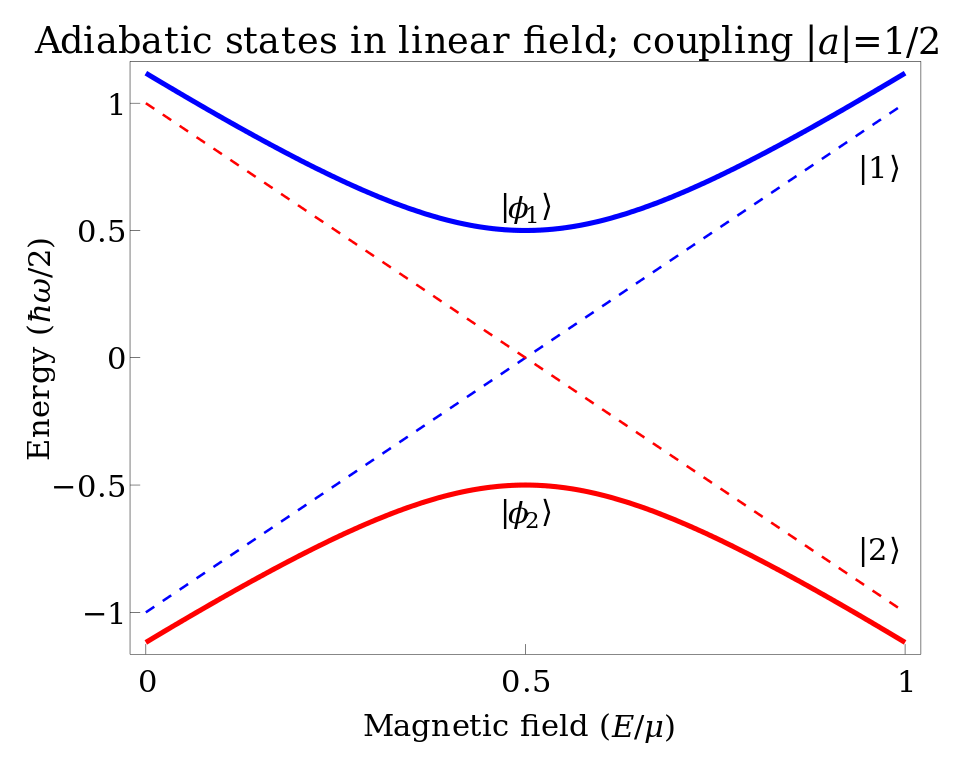
\includegraphics[scale=0.2]{img/Avoided_crossing_in_linear_field.svg.png}
    \end{center}
    Skizze zu einem Avoided Level Crossing eines Zwei-Niveau-Systems im magnetischen Feld. \refimgsource{Wikimedia}{https://commons.wikimedia.org/wiki/File:Avoided_crossing_in_linear_field.svg}{18.01.2022}{Creative Commons CC0 1.0 Universal Public Domain Dedication} 
\end{fquestion}

% \begin{question}{Was passiert jetzt wenn ich so einen strahl aus dem Feld herausbringe und mir den zeitlichen Verlauf der Mischungszustände und symmetriezustände anschaue?}
%     Da wusste ich nicht worauf sie hinaus wollten, sie wollten etwas über den mischungswinkel hören ???
    
%     Als Nächstes kam eine Frage, mit der ich erst nichts anzufangen wusste. Es ging so ungefähr wie: Was benötigt man denn, damit diese Spinzustände mischen, da Spinzustände ja eigentlich sonst Eigenzustände sind. Dann haben sie wieder etwas von energetisch und symmetrien gesprochen. Das waren wieder Signalworte. Kurz Hamilton skizziert wobei die planare Anisotropie nicht null sein darf, also die planare Anisotropie ist der "Wechselwirkungsterm" der dann zur Mischung führt. Damit waren sie zufrieden.
%     Und sie fragten noch, wie man diese Mischung denn dann beeinflussen kann. Dabei wollten sie darauf hinaus, dass man mithilfe von Magnetfeldern in der x-y-Ebene genau diese planare Anisotropie beinflusst.
% \end{question}

\subsection{Maser}

\begin{fquestion}{Wie funktioniert er?}
    % Skizze von Boltzmann-Verteilung N(E) ???
    % Besetzungsinversion für stimulierte Emission (siehe Laser: Pumpen), hier über Strahltrennung ???
    % Strahltrennung?
    % zu Beginn hohes Feld, damit Symmetrie den Energiezuständen entspricht ??? 
    % Strahlen mit einem inhomogenen eletrischen Feld trennen (ausnutzen, dass elektrische Dipolmomente der Symmetriezustände verschieden ausgerichtet sind -> Kraft von E-Feld unterschiedlich)
    % langsam elektrisches Feld senken, um wieder einen perfekt gemischten Zustand zu bekommen ??? 
    % im Hohlraumresonator und mit stimulierter Emission erhält man kohärentes Laserlicht (Mikrowellen, da maser, also meV)
    
    Der Aufbau besteht aus einem Strahltrenner mit inhomogenem elektrischen Feld $\epsilon_\text{inh.}$ und einer Kavität mit oszillierendem Feld $\epsilon_\text{ac}(t)$.
    \\
    Das Feld des Strahlteilers muss inhomogen sein, weil sich die Dipolmomente in einem homogenen Feld lediglich parallel zum Feld ausrichten.
    Damit eine Kraft entsteht, darf der Gradient des Felds also nicht verschwinden.
    In Abbildung \ref{fig:AmmoniakALC} befindet sich das System nun ganz rechts, wobei hier für die Eigenzustände näherungsweise $\ket{\psi_+}\approx \ket{1}$ und $\ket{\psi_-}\approx \ket{2}$ gilt (entspricht Mischungswinkel von $\theta\approx \SI{90}{\degree}$).
    Bei adiabatischer Absenkung des Feldes ``wandern'' die Zustände dann entlang der blauen Kurven, die den Eigenenergien 
    $$E_\pm = E_0 \pm \sqrt{A^2 + (\Vec{d}\cdot\Vec{\epsilon})^2}$$
    entsprechen.
    Für $\epsilon\approx 0$ befindet sich ein Großteil der Moleküle der beiden Strahle dann in einem der Eigenzustände wieder.
    \\
    Interessant ist hierbei der Anteil mit einer Eigenenergie von $E_0 + A$.
    Dieser wird nun in die Kavität geleitet.
    Mit etwas Mathematik kann man zeigen, dass die Periodendauer der angeregten Oszillation $T=\frac{\pi\hbar}{2|\Vec{d}||\Vec{\epsilon}_0|}$ entspricht.
    Die Moleküle sollten bei einer Geschwindigkeit $v$ und einer Länge der Kavität $L$ also gerade die Zeit $T$ in dieser verbringen, um (nahezu) vollständig in den niederenergetischen Eigenzustand $E_-$ überführt zu werden.
    Die Frequenz der dabei abgestrahlten Photonen ist $\omega = 2 A$.
\end{fquestion}

% NH3-Maser
\begin{figure}[!ht]
    \centering
    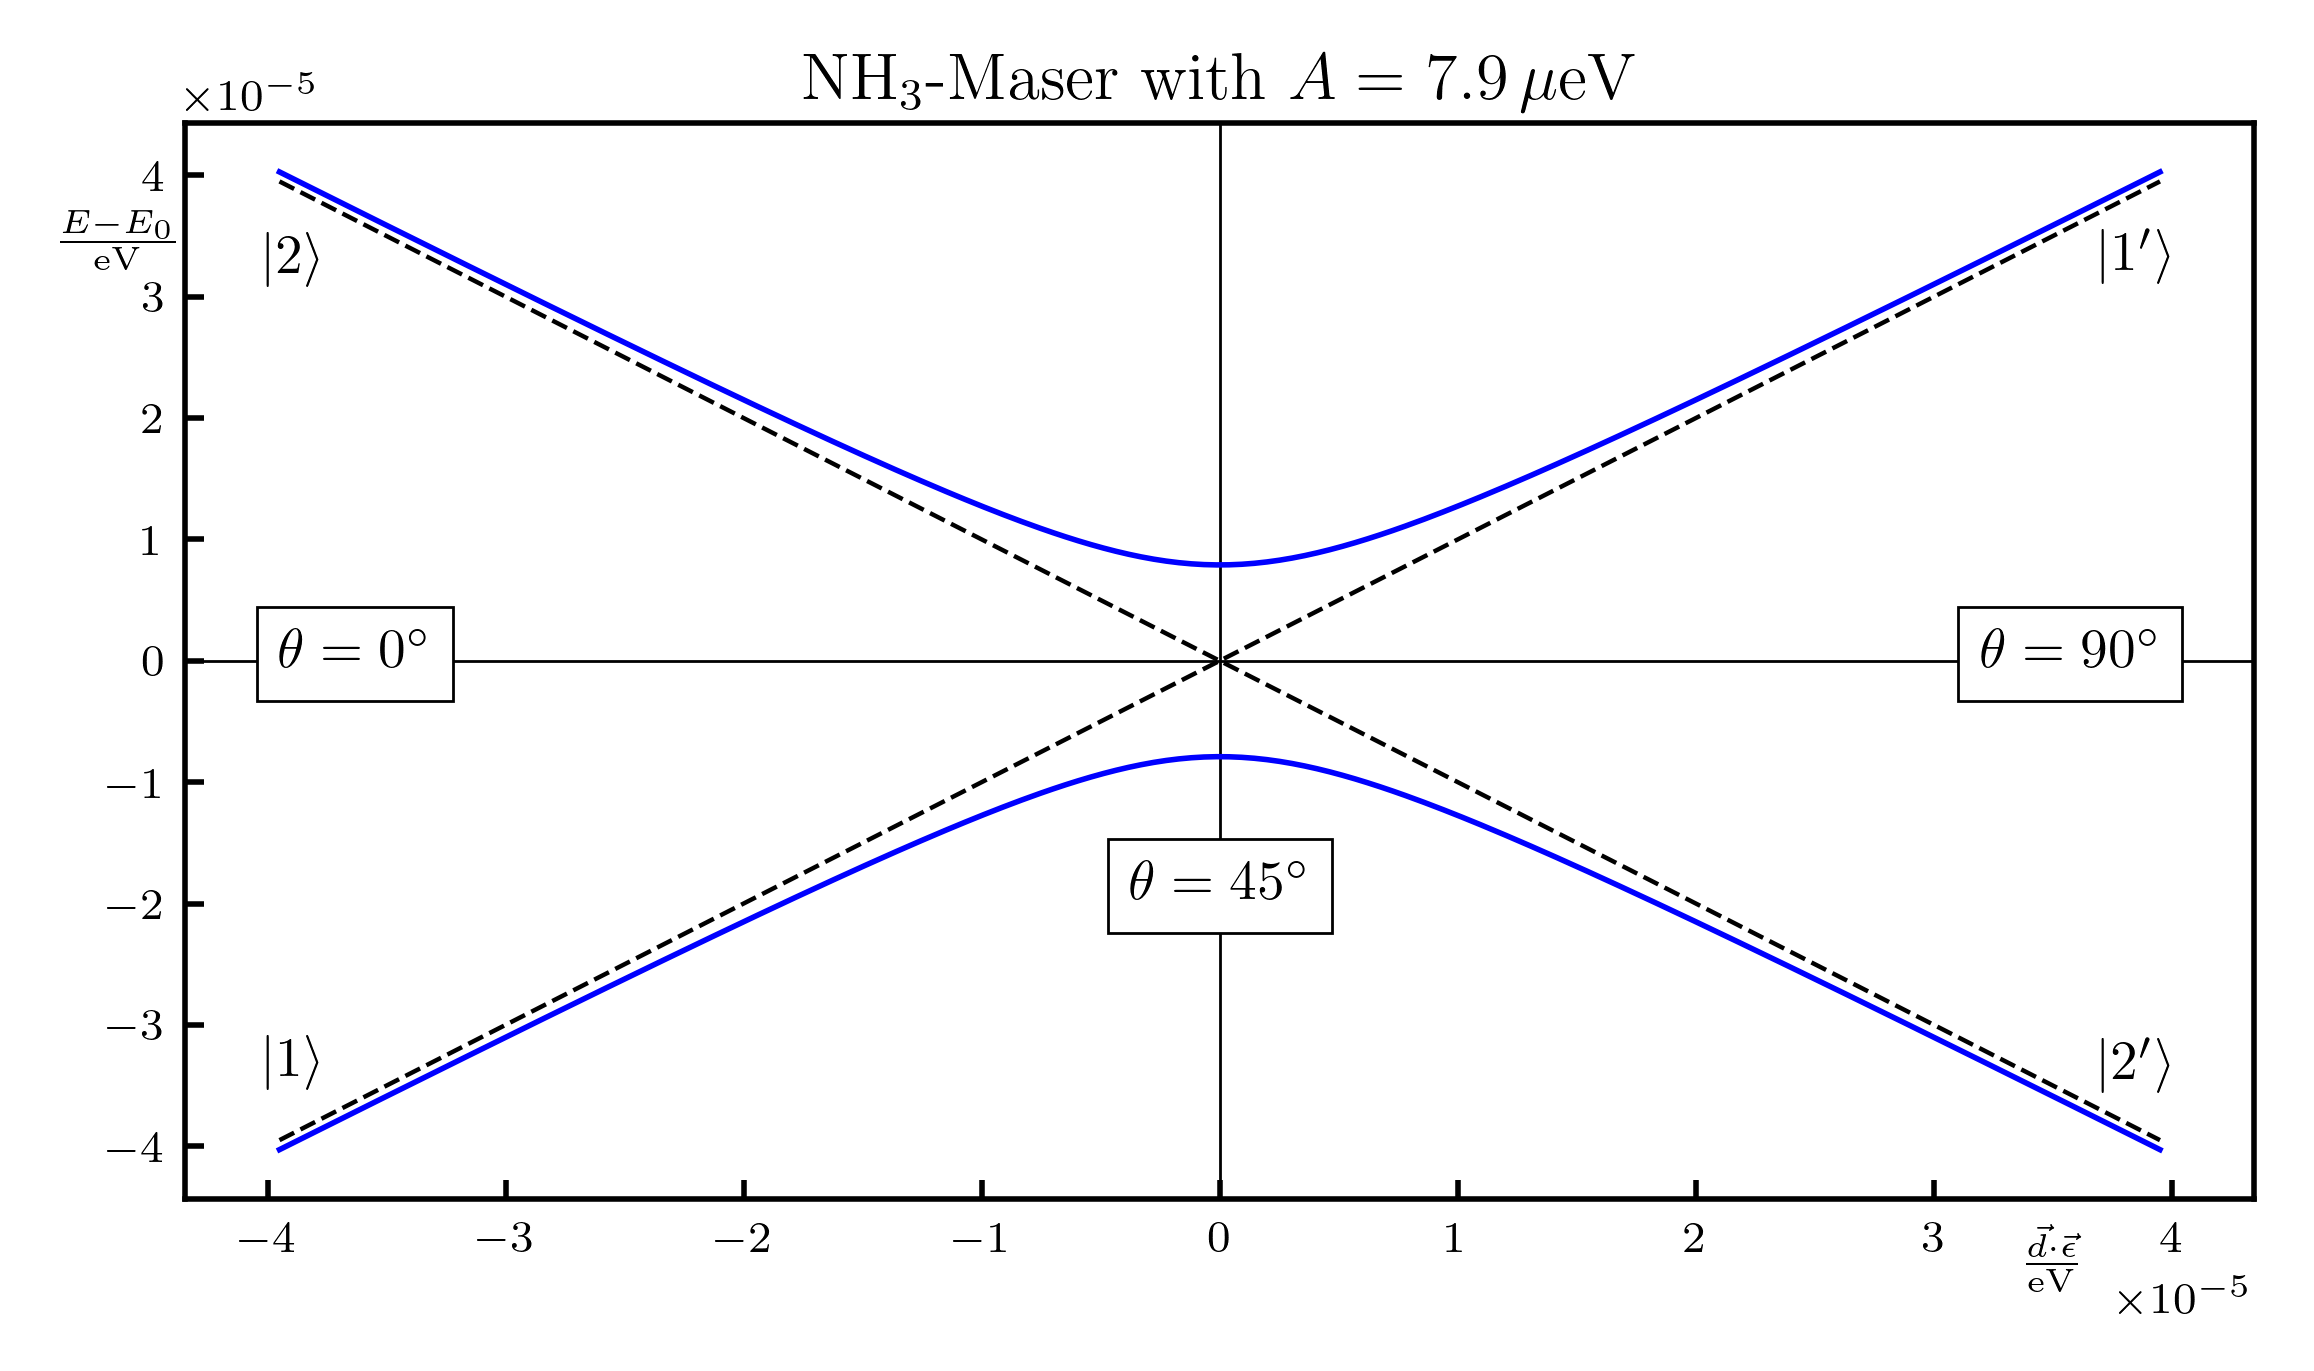
\includegraphics{img/AmmoniakALC.png}
    \caption{Vermiedene Kreuzungen für Ammoniak mit Dipolmoment $\Vec{d}$ in einem elektrischen Feld $\Vec{\epsilon}$.
    Der jeweilige Mischungswinkel ist als $\theta$ vermerkt.}
    \label{fig:AmmoniakALC}
\end{figure}

\begin{fquestion}{Warum inhomogenes Feld?}
    Im homogenen Feld nur Ausrichtung der Dipolmomente, aber keine Kraft.
\end{fquestion}

\begin{fquestion}{Warum sollte man das elektrische Feld langsam ändern?}
    Es tritt ein Landau-Zener Übergang mit der Tunnelwahrscheinlichkeit 
    \[P = e^{-\gamma}, \quad \gamma = \frac{|H_{12}|^2}{\dd E/\dd t}\]
    auf.
    Dieser ist abhängig von der Energie-Lücke, aber auch von der Energie-Änderungsrate.
\end{fquestion}

% \begin{question}{Wieso kommt es zum Aufspalten der Zustände?}
% \end{question}

% \begin{question}{Wie ist die Zustandsverteilung im oszillierenden Feld?}

% \end{question}

% \begin{question}{Die strahlenden Übergänge starten durch spontane Emissionen, dadurch werden wie bei laser weitere angeregt. Warum muss ich bei kleinen E-Feldern aufpassen?}
%     Langsam ändern lassen, damit nicht tunneln
% \end{question}

% \begin{question}{Energetische Betrachtung?}
%     Schema der vermiedenen Niveaukreuzungen
% \end{question}


\begin{fquestion}{Was sind andere Anwendungen des Masers?}
    Ein weiterer Maser ist der Wasserstoffmaser, bei dem die Hyperfeinstrukturaufspaltung von Wasserstoff im Grunzustand mit einer Frequenz 
    $$E_{\mathrm{HFS}} = \SI{1420405751.767}{Hz}$$
    genutzt wird.
    Zunächst werden die Atome im Zustand $F = 1$ (parallele Ausrichtung von Kern und Elektron) von denen im $F=0$ selektiert (etwa durch Zeeman-Aufspaltung im starken Magnetfeld).
    Eingeleitet in eine Kavität (mit Teflon beschichtet, damit die Wasserstoffmoleküle nicht binden können), herrscht dort eine Besetzungsinversion zwischen dem $F=1$ und $F=0$-Niveaus, wodurch eine stimulierte Emission mit genau der Hyperfeinstrukturaufspaltung beobachtet werden kann.
    
    Diese Frequenz ist so genau ($\mathcal{O}(10^{-12})$), dass sie zur präzisen Zeitmessung genutzt werden kann.
\end{fquestion}

% \subsection[${\text{Mn}}_{12}$-Acetat]{$\mathbf{\textbf{Mn}_{12}}$-Acetat}
% \subsection{$\mathbf{\textbf{Mn}_{12}}$-Acetat}
\subsection{Magnetische Moleküle}

\begin{figure}[htb]
    \centering
    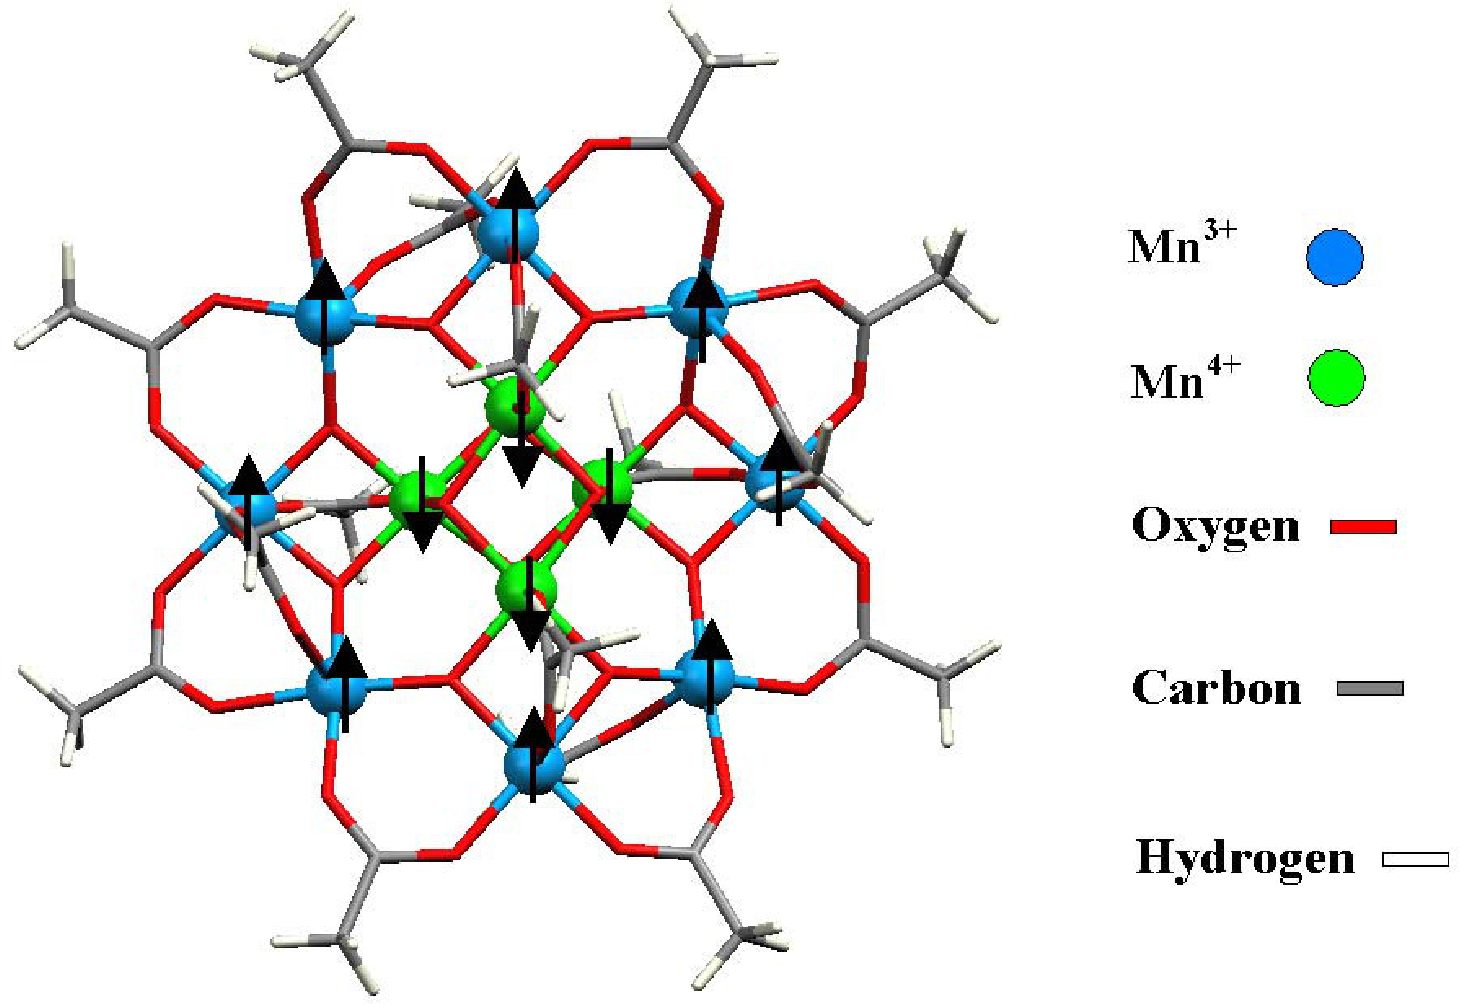
\includegraphics[width=0.5\linewidth]{img/17-Figure1.1-1.png}
    \caption{Skizze des $\text{Mn}_{12}$-Acetats. Dabei hat $\text{Mn}^{\text{III}}$ einen Spin von $s=2$ und $\text{Mn}^{\text{IV}}$ einen Spin von $s=3/2$.}
    \label{fig:mn12acetat}
\end{figure}

\begin{figure}
    \centering
    \begin{subfigure}{0.77\linewidth}
        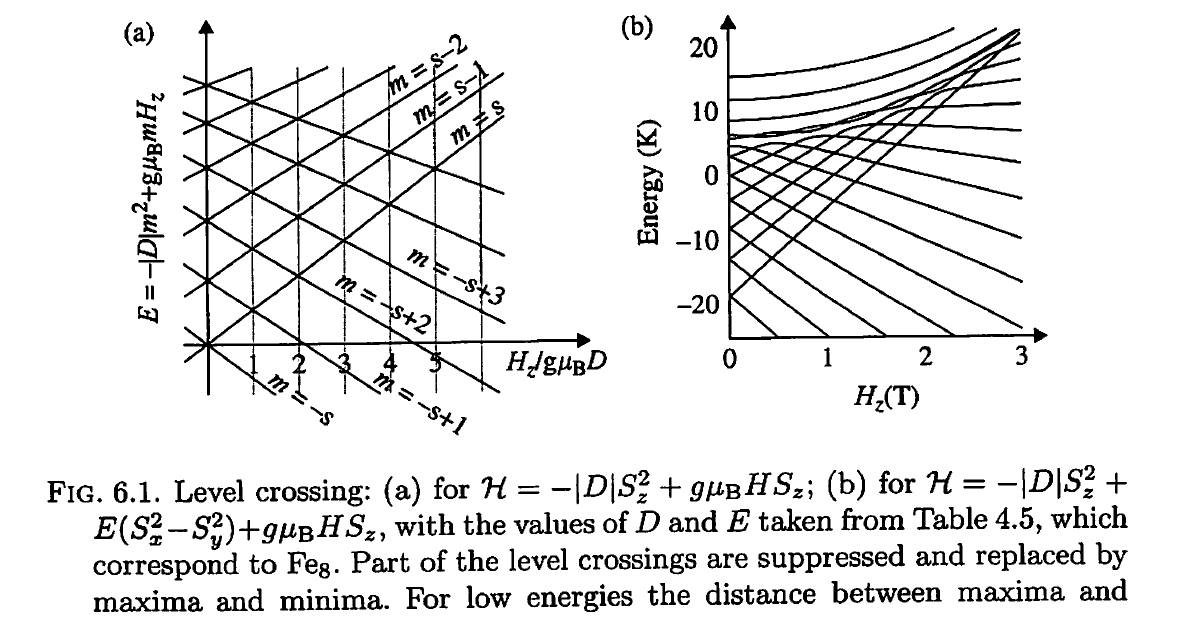
\includegraphics[width=\linewidth]{img/mn12_level_crossing.png}
    \end{subfigure}
    \begin{subfigure}{0.21\linewidth}
        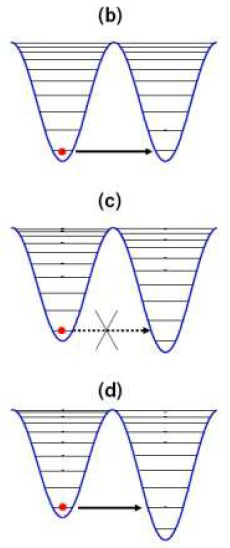
\includegraphics[width=\linewidth]{img/mn12_tunneling.png}
    \end{subfigure}
    \begin{subfigure}{0.9\linewidth}
        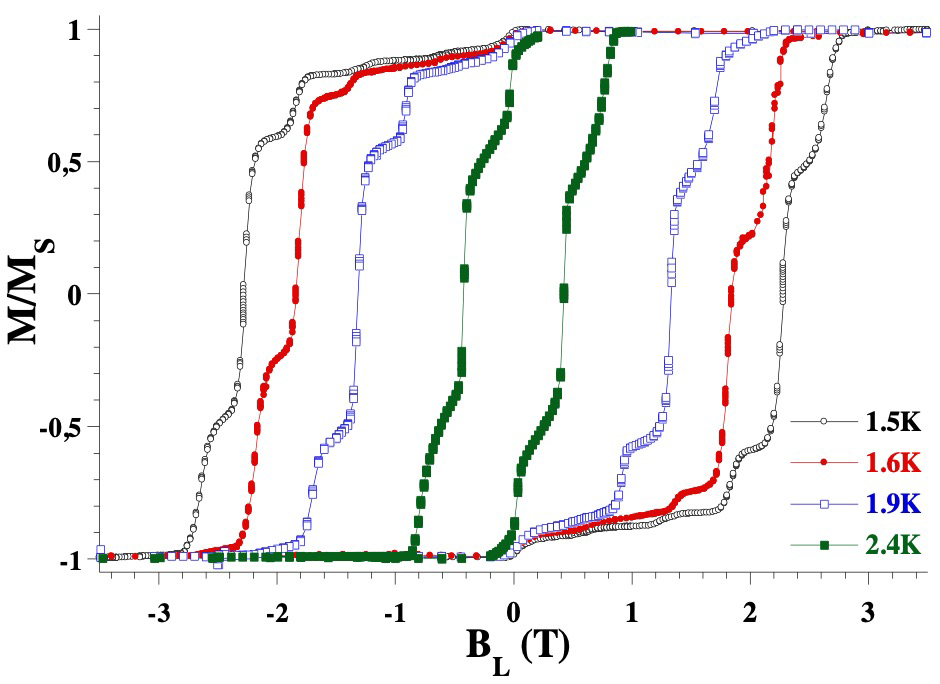
\includegraphics[width=\linewidth]{img/mn12_hysteresis.png}
    \end{subfigure}
    \caption{Übersicht über Energieniveauverlauf, Tunnelvorgang und Hysterekurve beim $\text{Mn}_{12}$-Acetat. Aus der Vorlesung entnommen.}
    \label{fig:mn12vis}
\end{figure}

\begin{fquestion}{Was misst man beim $\text{Mn}_{12}$-Acetat?}
    Beim magnetischen Molekül $\text{Mn}_{12}$-Acetat ($S = 10$) (alternativ auch beispielsweise beim $\text{Ni}$-Quadrumer oder beim $\text{V}_{15}$ ($S = 1/2$), $\text{Ni}_{12}$ ($S = 12$) oder $\text{Fe}_8$ ($S = 10$)) bilden sich entsprechend der Ausrichtung des Spins $m_s$ diskrete Magnetisierungen.
    Ohne externes Magnetfeld bilden diese unter dem Hamiltonian $H = -D S_z^2 + E (S_x^2 - S_y^2)$ zwei Parabeln mit entartetem Grundniveau $\ket{m_s = 10}$ und $\ket{m_s = -10}$.
    Wird ein externes Magnetfeld angelegt, wird durch $H = g \mu_B \mu_0 S H_{\text{ext}}$ die Entartung aufgehoben und bei bestimmten externen Magnetfeldern kreuzen sich die ursprünglichen Eigenzustände.
    
    An diesem Beispiel kann das Avoided-Level-Crossing sehr schön experimentell nachvollzogen werden, für Grafiken siehe \autoref{fig:mn12vis}.
\end{fquestion}

\subsection{Neutrinooszillation}

\begin{figure}[!ht]
    \centering
    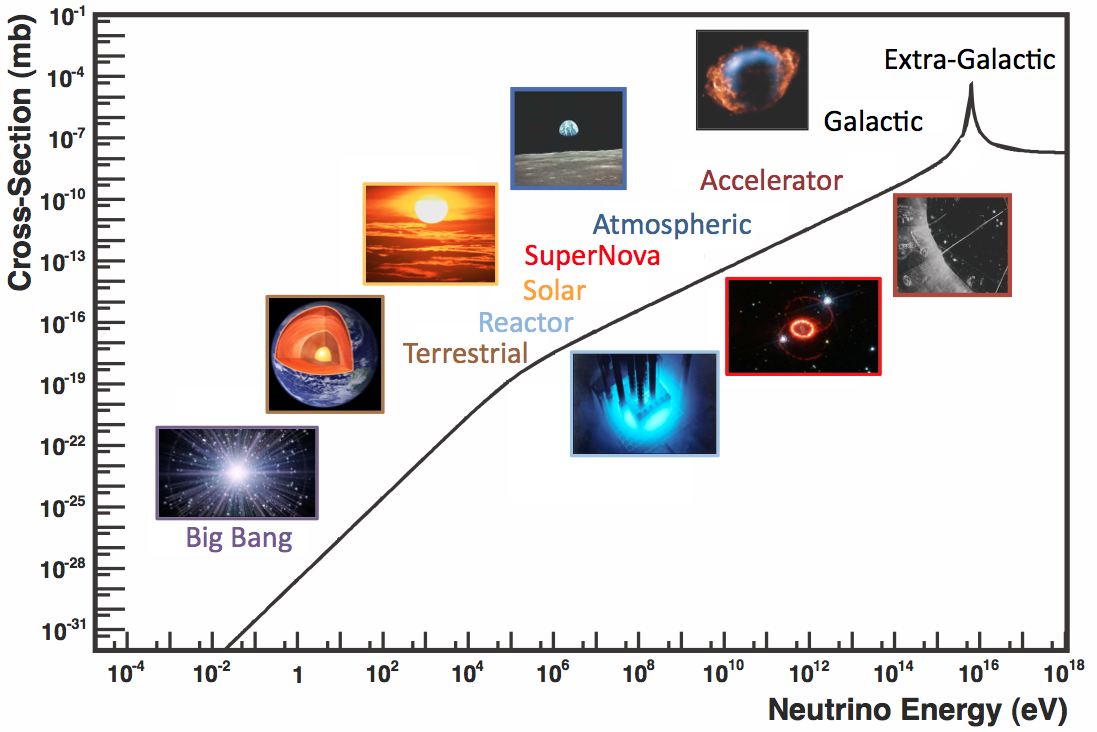
\includegraphics[width=\linewidth]{img/Neutrino_Wirkungswuerschnitt.png}
    \caption{Wirkungsquerschnitt von Neutrinos in Abhängigkeit der Energie mit $W^\pm$ Resonanz bei $\SI{10E16}{\electronvolt}$. Eine mögliche Quelle der Neutrinos mit entsprechenden Energien ist vermekt.
    \refimgsource{From eV to EeV: Neutrino Cross-Sections Across Energy Scales}{https://arxiv.org/pdf/1305.7513.pdf}{18.01.2022}{keine}}
\end{figure}

\begin{fquestion}{Wieso gibt es bei den Neutrinos Zustandsmischungen?}
    Entsprechend der PMNS (Pontecorvo–Maki–Nakagawa–Sakata) Matrix
    \[U_{\mathrm{PMNS}} \approx \begin{pmatrix}
        0.8 & 0.6 & 0.1 \\
        0.4 & 0.5 & 0.7 \\
        0.4 & 0.5 & 0.7 
    \end{pmatrix}\]
    mit den Mischwinkeln $\theta_{12} = \SI{33}{\degree}$, $\theta_{23} = \SI{49}{\degree}$ und $\theta_{13} = \SI{9}{\degree}$ sind die Flavoureigenzustände aus Masseneigenzuständen ${\nu_{\mathrm{Flavour}} = U_{\mathrm{PMNS}} \nu_{\mathrm{Masse}}}$ zusammengesetzt. 
    Letztere breiten sich mit unterschiedlichen Frequenzen entsprechend der Energien aus, wodurch es zu Intereferenzen kommt.
    In der Flavourprojektion zeigen sich diese durch Oszillationen zwischen verschiedenen Flavourzuständen.
\end{fquestion}

\begin{fquestion}{Wie kommt die Oszillation aus der Zeitentwicklung zustande?}
    Die Eigenzustände entwickeln sich gemäß $\ket{\nu_{1,2}(t)} = \e^{-\i E_{1,2}t} \ket{\nu_{1,2}},$ wobei die Eigenenergien durch 
    $$E_{1,2} = \sqrt{m_{1,2}^2 + p^2} \approx p + \frac{m_{1,2}^2}{2p} $$
    gegeben sind.
    Hierbei ist insbesondere die Energiedifferenz relevant, welche über $\Delta m_{12}^2 = m_2^2 - m_1^2 \approx \SI{7.5e-5}{eV^2}$ gegeben ist.
    Da im Vakuum $\ket{\nu_e} = \cos\theta_{12}\ket{\nu_1} + \sin\theta_{12}\ket{\nu_2}$ ist, folgt die Zeitentwicklung entsprechend
    $$\ket{\nu(t)} = \e^{-\i E_{1}t} \cos\theta_{12}\ket{\nu_1} + \e^{-\i E_{2}t} \sin\theta_{12}\ket{\nu_2}.$$
    % psi(t) = c1(t) |1> + c2(t) |2> und wie c1 und c2 aussehen und warum (also kurz für Eigenzustände Zeitentwicklung benannt)
    % Koeffizienten über Anfangsbedingung
    Die Neutrinos bewegen sich beinahe mit Lichtgeschwindigkeit, also  $v \sim c$.
    Damit können wir anstatt Zeit auch Entfernung betrachten, also $ t\sim x$ (z.B. bei atmosphärischen Neutrinos gut zu erkennen). 
    Die Überlebenswahrscheinlichkeit ist dann gegeben durch
    $$P_{ee}(x) = |\braket{\nu_e }{ \nu (x)}|^2 = \left\vert \e^{-\i \frac{m_1^2}{2E}x} \cos^2\theta_{12} + \e^{-\i \frac{m_2^2}{2E}x} \sin^2\theta_{12} \right\vert^2.$$
    Eine ausführliche Rechnung liefert dann
    $$P_{ee}(x) = 1 - \sin^2 2\theta_{12} \sin^2\left( \frac{\Delta m_{12}^2}{4E} x \right).$$
\end{fquestion}

\begin{fquestion}{Was ist der Störparameter bei der Neutrinooszillation?}
    Die Elektronendichte (bei $\nu_e$-Oszillation) des umliegenden Mediums.
\end{fquestion}

\begin{fquestion}{ALC in der Sonne, was passiert da genau?}
    % Elektronneutrino zu Myonneutrino  (auch tau)
    Durch die Elektronendichte $n_e(r) = n_0\e^{-r/r_0}$ gibt es in der Sonne einen zusätzlichen Term, der zur Masse der Elektronneutrinos beiträgt $$\Delta m_N^2(r) = 2E\sqrt{2}G_F n_e(r).$$
    Im Vakuum gilt
    $$\begin{pmatrix}
     | \nu_e \rangle \\  | \nu_\mu  \rangle
    \end{pmatrix} = \begin{pmatrix}
    \cos\theta & \sin\theta \\ -\sin\theta & \cos\theta
    \end{pmatrix} \begin{pmatrix}
     | \nu_1 \rangle \\  | \nu_2 \rangle
    \end{pmatrix},$$
    wobei durch die Materie der Mischungswinkel verändert wird.
    Die Erwartungswerte der Massen der Flavour-Neutrinos sind hier
    $$m_{\nu_e}^2 = \langle \nu_e | \hat{m}^2 | \nu_e \rangle = m_{\nu_1}^2 \cos^2\theta + m_{\nu_2}^2 \sin^2\theta = \Delta m_{12}^2 \sin^2\theta + m_{\nu_1}^2,$$
    $$m_{\nu_\mu}^2 = \langle \nu_\mu | \hat{m}^2 | \nu_\mu \rangle = m_{\nu_1}^2 \sin^2\theta + m_{\nu_2}^2 \cos^2\theta = \Delta m_{12}^2 \cos^2\theta + m_{\nu_1}^2.$$
    Wegen des MSW-Effekt (Michejew-Smirnow-Wolfenstein) ändern sich die Massen-Eigenzustände zu
   $$\tilde{m}^2_{\nu_1,\nu_2} - m_{\nu_1}^2 = \frac{1}{2}\left( \Delta m_{12}^2 + \Delta m_N^2(r) \pm \Delta \tilde{m}^2(r) \right),$$
    wobei die Massen-Lücke durch
    $$\Delta \tilde{m}^2(r) = \sqrt{\left( \Delta m_{12}^2 \cos 2\theta_{12} - \Delta m_N^2 (r) \right)^2 + \left( \Delta m_{12}^2 \sin 2\theta_{12} \right)^2 }$$
    Abbildung \ref{fig:solar neutrino msw theta 34} zeigt die Entwicklung der Zustände in der Sonne.
\end{fquestion}

\begin{figure}[!ht]
    \centering
    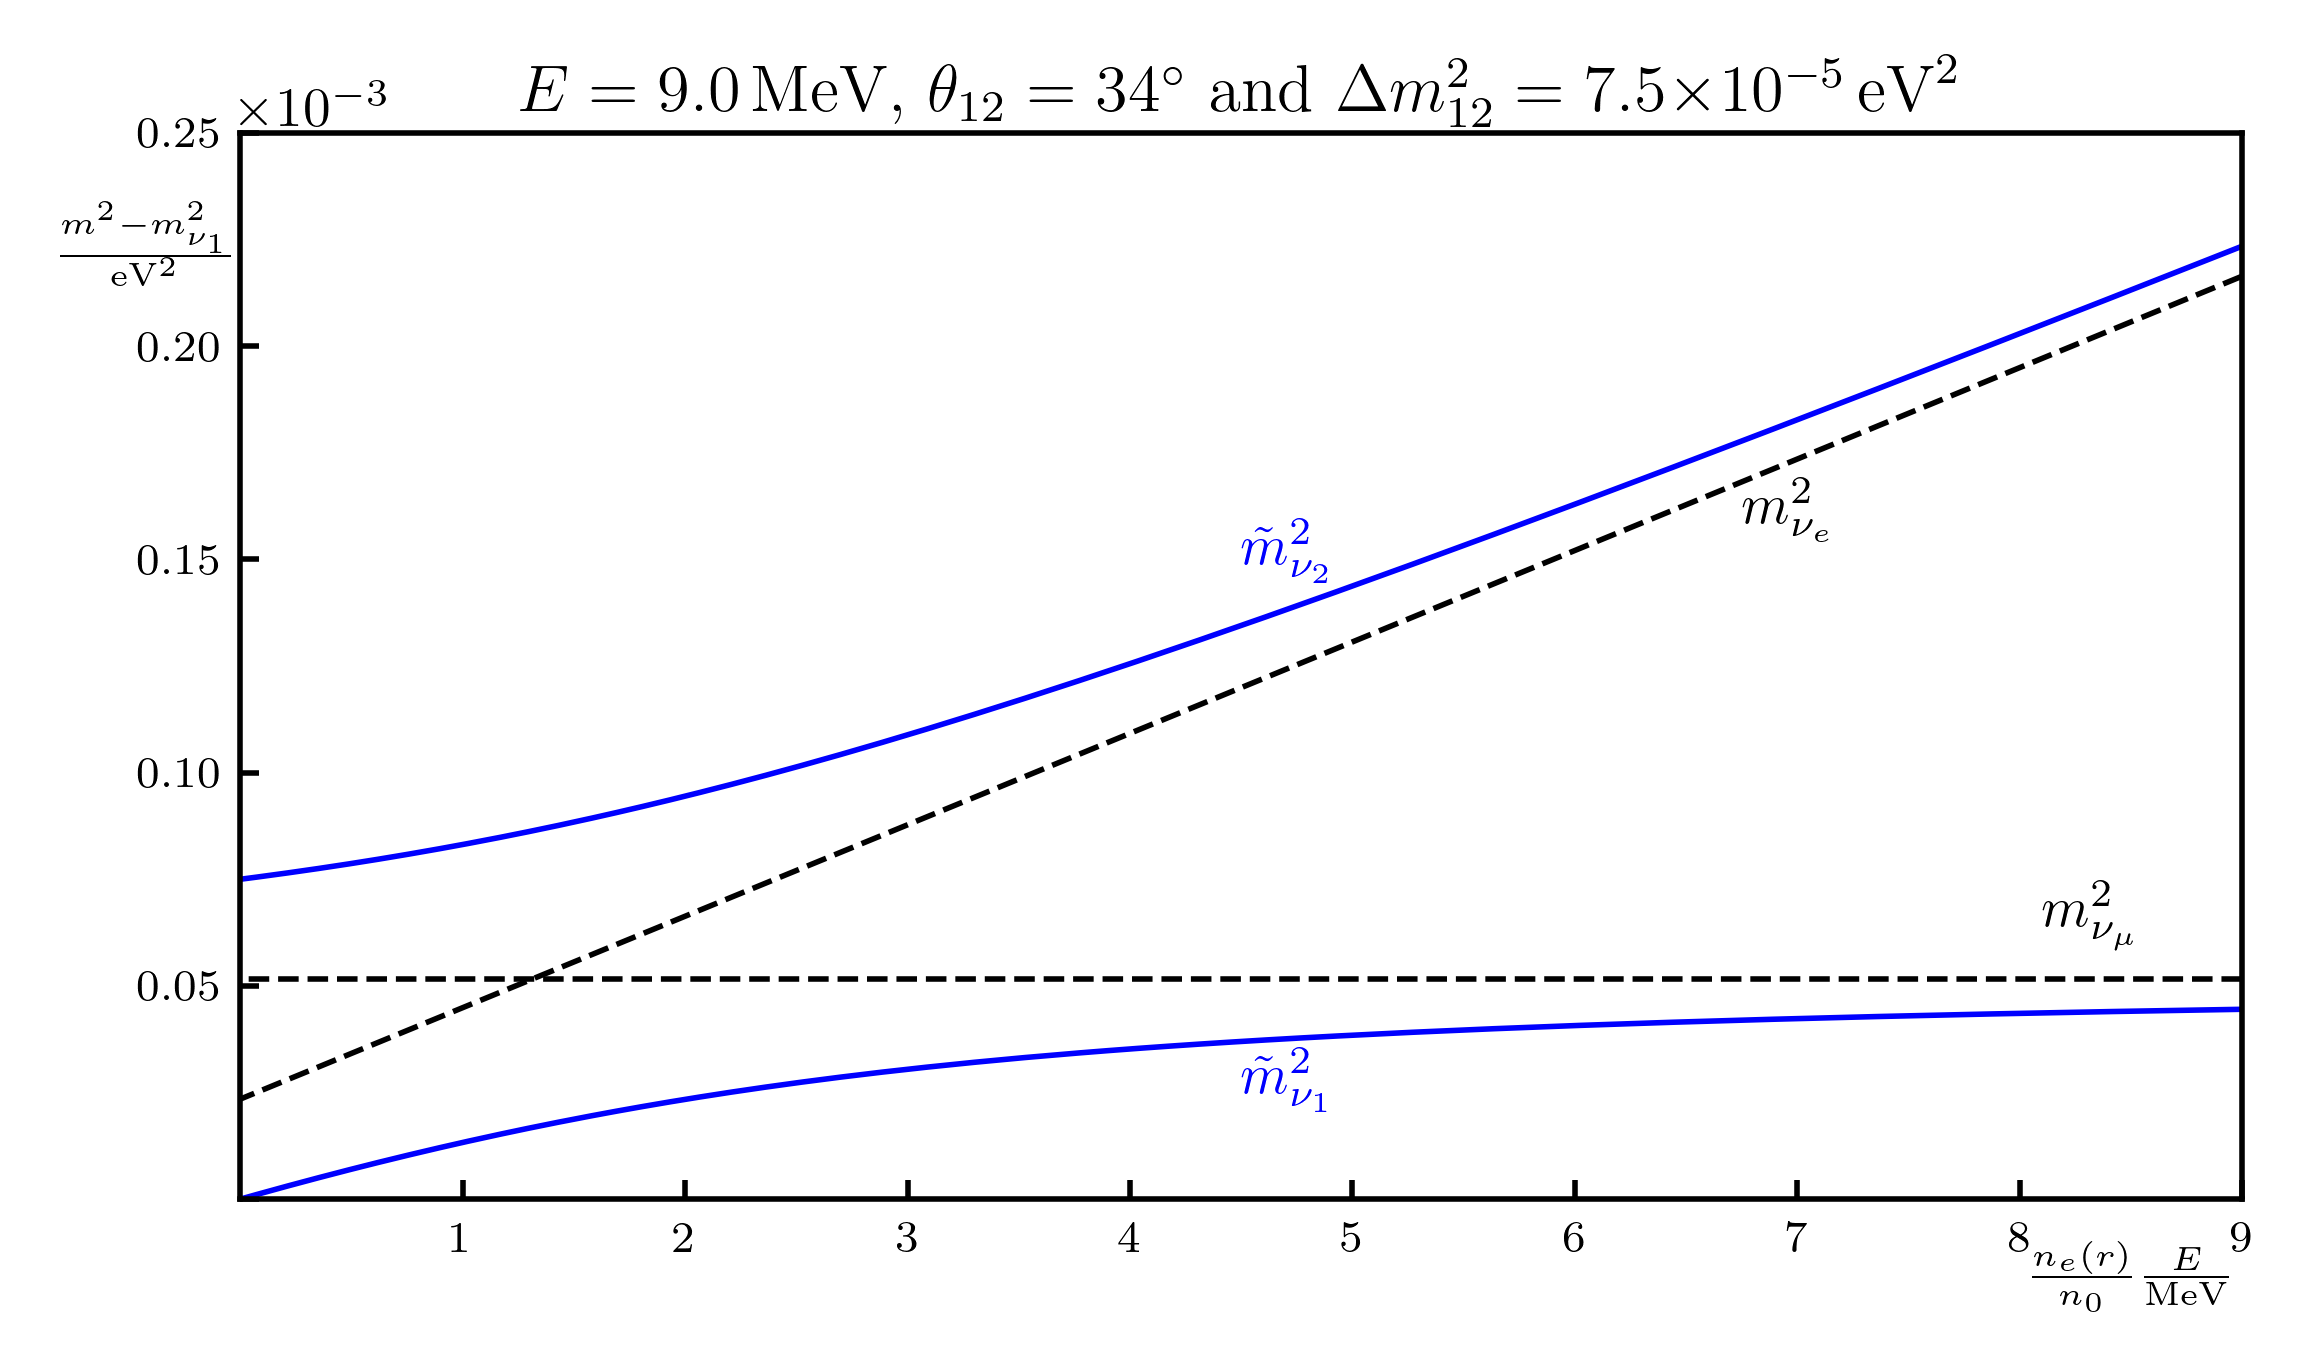
\includegraphics{img/SolarNeutrinoALC_theta34v3.png}
    \caption{Visualisierung der Entwicklung der Massen-Eigenzustände $ | \tilde{\nu}_{1,2} \rangle$ in der Sonne.
    Die $x$-Achse entspricht der Elektronendichte, das Sonnenzentrum ist also rechts, das (fast-)Vakuum links.}
    \label{fig:solar neutrino msw theta 34}
\end{figure}

\begin{fquestion}{Was sind jeweils die geraden Linien im Diagramm}
    Die Erwartungswerte der Massen der Flavour-Eigenzustände.
    Der für das Elektron-Neutrino hängt von der Elektronendichte ab.
    Der Kreuzungspunkt wandert für höhere Energien nach links, also zum Sonnenrand hin, weil der Anstieg der $\nu_e$-Geraden größer wird.
\end{fquestion}


\begin{fquestion}{Was ist der MSW-Effekt?}
    Beschreibt den Einfluss von Materie auf die Neutrino-Oszillationen. 
    Durch die Elektronendichte erhält der Elektron-Neutrino Zustand eine zusätzliche Masse über die Wechselwirkung mit $W^\pm$.
    Das Feynman-Diagramm für Geladene Ströme (also über $W^\pm$) ist für Myon- und Tau-Neutrinos nicht möglich.
\end{fquestion}

\begin{fquestion}{Was ist die Ursache dafür?}
    Aufgrund der Erhaltung der Flavour-Zahl ist das Feynman-Diagramm für die Streuung der anderen Neutrinos an Elektronen über $W^\pm$ verboten.
\end{fquestion}

\begin{fquestion}{Warum gibt es denn nur Elektronen in der Sonne?}
    Energie der solaren Neutrinos liegt in der Größenordnung  $1\dots 10\,$MeV, also deutlich unterhalb der Masse von Myonen oder Taus.
\end{fquestion}

\begin{fquestion}{Wie werden Neutrinos in der Sonne produziert?}
    Die dominierende Reaktionsgleichung lautet
    \[p + p \rightarrow d + e^+ + \nu_e.\]
    Es verschmelzen zwei Protonen zu einem Deuterium-Kern, einem Positron und einem $e$-Neutrino.
    Das entsprechend Feynman-Diagramm ist in \autoref{fig:neutrino_prod_sonne}.

    Die weiteren Prozesse sind die folgenden:
    
    \begin{center}
        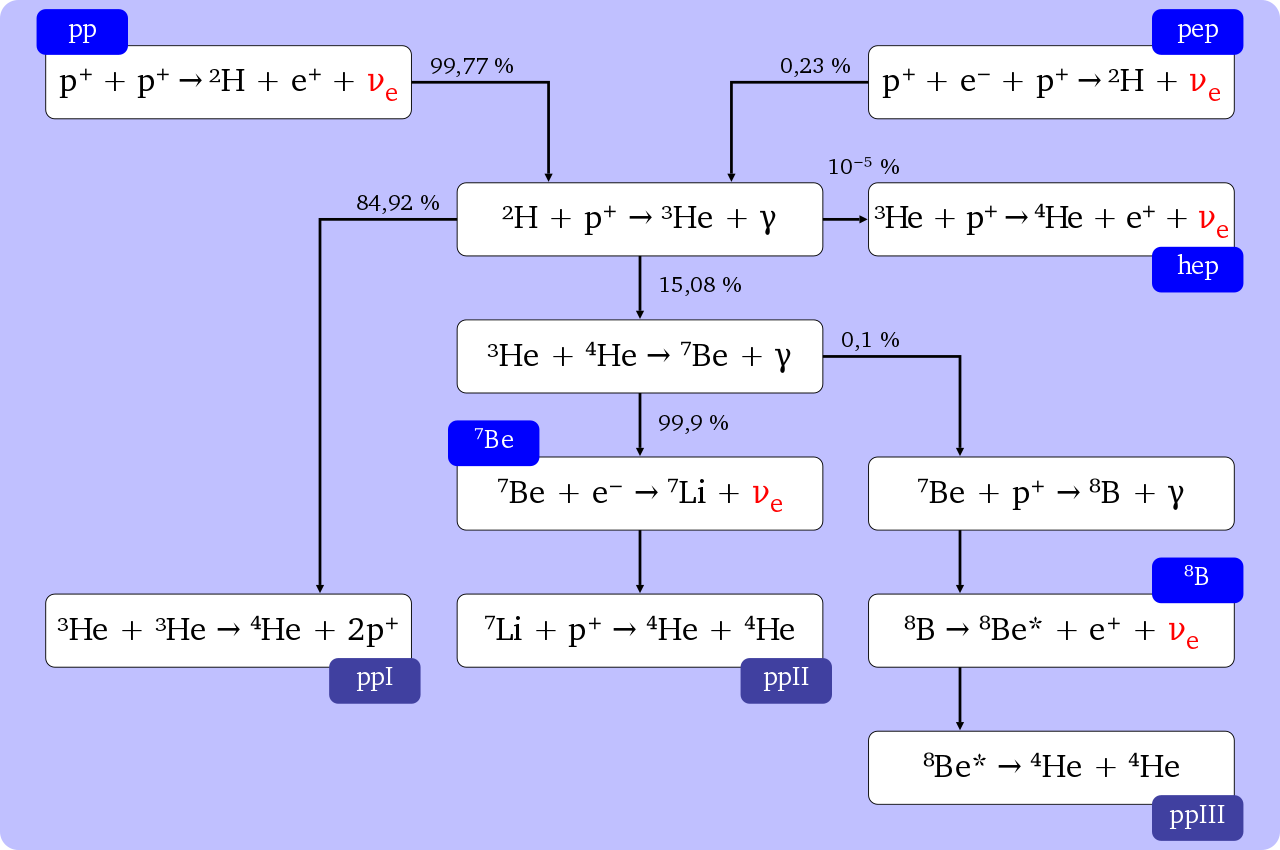
\includegraphics[width=.9\linewidth]{img/1280px-Proton_proton_cycle.svg.png}
    \end{center}
    
    \refimgsource{Wikimedia}{https://upload.wikimedia.org/wikipedia/commons/thumb/a/ac/Proton_proton_cycle.svg/1280px-Proton_proton_cycle.svg.png}{20.01.2022}{Creative Commons Attribution-Share Alike 2.5 Generic}

\end{fquestion}

\begin{figure}[!ht]
    \centering
    % 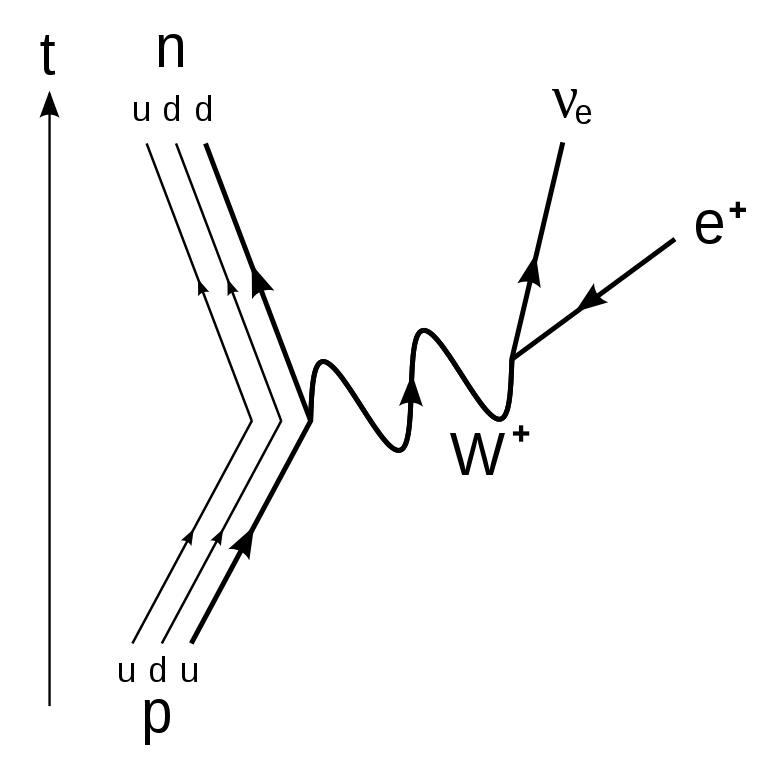
\includegraphics[scale=0.3]{img/768px-Electron_Capture_Decay.svg.png}
\begin{tikzpicture}[x=20mm, y=20mm]
\begin{feynman}[]
    \vertex (i1) {\(u\vphantom{d}\)};
    \vertex[right=.15 of i1] (i2) {\(d\)};
    \vertex[right=.15 of i2] (i3) {\(u\vphantom{d}\)};
    \vertex[below=.3 of i2] (n) {\(p\)};

    \vertex[above=2 of i1] (f1) {\(u\vphantom{d}\)};
    \vertex[right=.15 of f1] (f2) {\(d\)};
    \vertex[right=.15 of f2] (f3) {\(d\)};
    \vertex[above=.3 of f2] (p) {\(n\)};

    \vertex[above=1 of i3] (a);
    \vertex[right=.15 of a] (b);
    \vertex[right=.15 of b] (c);

    \vertex at ($(c) + (.7,.25)$) (d);
    \vertex at ($(d) + (.2, 1)$) (f4) {\({\nu}_e\)};
    \vertex at ($(d) + (.9,.5)$) (f5) {\(e^+\)};
\diagram*{
    (i1) -- [fermion] (a) -- [fermion] (f1),
    (i2) -- [fermion] (b) -- [fermion] (f2),
    (i3) -- [fermion, thick] (c) -- [fermion, thick] (f3),
    (c) -- [boson, edge label'=\(W^+\), thick] (d) -- [fermion, thick] (f5),
    (d) -- [anti fermion, thick] (f4),
};

\draw[-{Stealth[width=2mm, length=3mm]},thick] (-.4,-.4) -- (-.4,2.2);
\node at (-.4,2.3) {\(t\)};
\end{feynman}
\end{tikzpicture}


    \caption{Feynman-Diagramm erster Ordnung für die Umwandlung eines Protons in ein Neutron unter Abgabe eines Elektronneutrinos.}
    \label{fig:neutrino_prod_sonne}
\end{figure}

\begin{fquestion}{Wie ist das Verhältnis von $\nu_\mu$ und $\nu_e$ aus der Atmosphäre?}
    Das Verhältnis ist etwa $2 \nu_\mu : 1 \nu_e$.
    Dies kommt aus der Reaktionskette in der Atmosphäre:
    \[ p + \mathrm{Nukleon} \rightarrow n + \pi, \quad \pi \rightarrow \mu + \overline{\nu}_\mu, \quad \mu \rightarrow e^- + \overline{\nu}_e + \nu_\mu \]
    
    Dabei kommen weniger $\mu$-Neutrinos ``von unten'', weil die sich in $\tau$-Neutrinos umwandeln (MSW in Erde).
\end{fquestion}

\begin{fquestion}{Wie kann man solare Neutrinos auf der Erde detektieren?}
    Durch inversen beta-Zerfall, beispielsweise Homestake ($E_\nu \ge \SI{0.814}{MeV}$)
    $$\nu_e + {}^{37}\mathrm{Cl} \rightarrow {}^{38}\mathrm{Ar}^+ + e^-,$$
    oder Gallex ($E_\nu \ge \SI{0.233}{MeV}$)
    $$\nu_e + {}^{71}\mathrm{Ga} \rightarrow {}^{71}\mathrm{Ge}^+ + e^-.$$
    Super-Kamiokande misst hingegen mit Photomultipliern die Tscherenkov-Strahlung von Elektronen, die von einem Neutrino gestreut wurden.
    Für Energien von einigen MeV wird das Elektron dabei auf mehr als 75\,\% der Lichtgeschwindigkeit beschleunigt, womit in Wasser Tscherenkov-Strahlung auftritt.
    \\
    Das Sudbury-Neutrino-Observatory (SNO) verwendet schweres Wasser ($\mathrm{D}_2$O) um sogar zwei Umwandlungsprozesse zu ermöglichen.
    Elektron-Neutrinos können über geladene Ströme ein Neutron in ein Proton gemäß
    $$\nu_e + D \rightarrow 2p + e^-$$
    umwandeln, wobei das Elektron wieder über die Tscherenkov-Strahlung erkannt wird.
    Alle Neutrinos können zusätzlich über neutrale Ströme gemäß
    $$\nu_x + D \rightarrow p + n + \nu_x$$
    an einem Deuteron streuuen, wobei dieses in Proton und Neutron zerfällt.
    Das Neutron wird von einem Deuteron eingefangen, wobei sich das entstehende Triton unter Emission eines Photons mit 2\,MeV wieder abregt.
\end{fquestion}

\begin{fquestion}{Was ist das solare Neutrinoproblem?}
    Es wurden weniger Elektron-Neutrinos gemessen, als gemäß des Modells der Sonne erwartet waren. 
    Homestake (etwa 33\,\%), Gallex (etwa 61\,\%) und Super-Kamiokande (etwa 46\,\%) haben dabei sogar deutlich verschiedene Abweichungen gemessen.
    \\
    Durch die Neutrinooszillation wird ein Teil der in der Sonne produzierten Elektron-Neutrinos in Myon- oder Tau-Neutrino umgewandelt.
    Durch den MSW-Effekt ist der Anteil energieabhängig, was die Diskrepanz der Experimente erklärt (Messung bei unterschiedlichen Neutrino-Energien).
\end{fquestion}

% \begin{question}{Wie misst man eigentlich verschiedene Neutrinoflavours?}
%     Elektron-Neutrino wechselwirkt mit Kernen und ändert z.B. Neutron im Kern zu Proton + Elektron
%     andere Neutrinos genau so, aber zu wenig Energie für Myonen/Tau's
% \end{question}

\begin{fquestion}{Kann man die Detektierung auch mit Myon-Neutrinos und Myonen machen? }
    Grundsätzlich ja, aber die solaren Neutrinos haben nicht genug Energie, um die Ruhemasse von Myonen aufzubringen.
\end{fquestion}

% \begin{question}{Warum nur so wenige Elektron-neutrinos? }
%     Oszillation
% \end{question}

% \begin{question}{Wovon hängt ab, ob die Elektron-Neutrinos zu Myon-Neutrinos werden? }
%     Dichte der Elektronen in Sonne muss sich langsam ändern, also dürfen die Neutrinos nicht zu viel Energie haben
% \end{question}

% \begin{question}{Aber die fliegen doch mit quasi Lichtgeschwindigkeit, wieso kann man trotzdem von einer langsamen Änderung ausgehen? }
%     Weil der Sonnenradius so riesig ist
% \end{question}

\subsection{Neutrale Kaonen}

\begin{fquestion}{Wie können Zustandsmischungen beim neutralen Kaon auftreten?}
    Das neutrale Kaon hat zwei Zustände:
    \[|\mathrm{K}^0 \rangle = |\mathrm{d} \bar{\mathrm{s}}  \rangle \qquad |\bar{\mathrm{K}}^0 \rangle = |\bar{\mathrm{d}} \mathrm{s} \rangle \qquad (\text{Masse } m = \SI{497}{\mega\electronvolt}).\]
    
    Durch den Austausch zweier $W$-Bosonen können die Zustände mischen.
    Diese Oszillation findet mit einer Frequenz von ungefähr $\SI{4}{\giga\hertz}$ statt.
    \begin{center}
        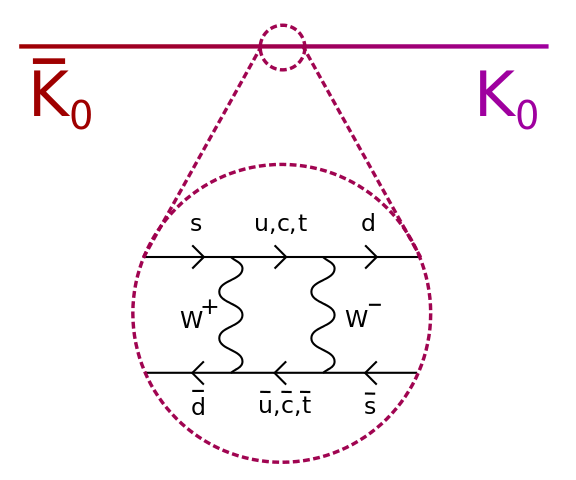
\includegraphics[width=0.4\linewidth]{img/Kaon-box-diagram-with-bar.svg.png}
    \end{center}
    \refimgsource{Wikimedia}{https://commons.wikimedia.org/wiki/File:Kaon-box-diagram-with-bar.svg}{24.01.2022}{Creative Commons Attribution-Share Alike 3.0 Unported}
\end{fquestion}

\begin{fquestion}{Wie wird dort die $CP$ Symmetrie gebrochen?}
    Unter der Parität $P$ und der Ladungskonjugation $C$ haben die beiden Kaonen die Abbildungsgleichung
    $$
    \begin{aligned}
        CP \ket{K^0} &= -\ket{\bar{K}^0}, &&& CP \ket{\bar{K}^0} &= -\ket{K^0}
    \end{aligned}
    $$
    Die Eigenzustände der $CP$ Operation sind entsprechend
    $$
    \begin{aligned}
        \ket{K_1^0} &= \frac{1}{\sqrt{2}} \left(\ket{K^0} - \ket{\bar{K}^0} \right), &&& \ket{K_2^0} &= \frac{1}{\sqrt{2}} \left(\ket{K^0} + \ket{\bar{K}^0} \right)
    \end{aligned}
    $$
    mit
    \(CP\ket{K_1^0} = + \ket{K_1^0}\) und \(CP\ket{K_2^0} = -\ket{K_2^0}\)
    Unter Annahme der $CP$ Erhaltung ergeben sich die beiden Zerfallskanäle $K_1^0 \rightarrow 2 \pi$ (schnell) und $K_2^0 \rightarrow 3\pi$ (langsam).
    In der Realität existieren ein langlebiger $K^0_L$ und ein kurzlebiger $K^0_S$ Kaonzustand, allerdings kann der langlebige ebenfalls in $2\pi$ zerfallen, weswegen dies keine $CP$ Eigenzustände sind und die Symmetrie entsprechend gebrochen ist.
\end{fquestion}

% \begin{question}{Wie sieht das bei Kaonen aus?}
%     Umwandlungsschema (Feynman-Diagramme), k und anti-K vs. $K_\text{short}$ und $K_\text{long}$
% \end{question}

\subsection{Laser}

\begin{fquestion}{Wie beschreibt man ein 2-Niveau System?}
    In einem 2-Niveau System gibt es drei Prozesse bei dem Übergang zwei Niveaus $N_1$ und $N_2$ ($E_1 < E_2$): Absorption $B_{12}$, sowie spontane $A_{21}$ und stimulierte $B_{21}$ Emission (mit den jeweiligen Einstein-Koeffizienten).
    Daraus ergibt sich die Ratengleichung
    $$\dot{N}_1 = -\dot{N}_2 = -B_{12} u N_1 + B_{21} u N_2 + A_{21} N_2$$
    in Abhängigkeit der spektralen Energiedichte $u$.
    Nach längerem Rechnen (mit der Boltzmann-Verteilung der Energieniveaus) erhält man $B_{12} = B_{21}$ (bei gleicher Entartung der Energieniveaus) und $A_{21} = \frac{8\pi h}{\lambda^3} B$.
    Außerdem erhält man im thermodynamischen Gleichgewicht 
    $$\frac{N_2}{N_1} = \frac{B_{12} u}{A_{21} + B_{21} u}$$
    was insbesondere mit den obigen Bedingungen bedeutet dass $N_2 < N_1$ und damit nie mehr Photonen stimuliert emittiert als absorbiert werden können.
\end{fquestion}

\begin{fquestion}{Wie funktioniert ein Laser?}
    Ein Laser funktioniert über die sogenannte \textit{Besetzungsinversion}. 
    Bei etwa einem 3- oder 4-Niveau-System kann es technisch erreicht werden, dass das Laserniveau $N_L$ höher bevölkert als der niedrigere Zustand ist.
\end{fquestion}

\begin{fquestion}{Wie sind die Übergänge bei einem 3-Niveau-Laser?}
    Bei einem 3-Niveau Laser gibt es drei Energieniveaus $E_1 < E_2 < E_3$. 
    Der Laser funktioniert dann über
    $$E_1 \xrightarrow{\text{Pumpen}} E_3 \xrightarrow[\text{Spontan}]{\text{Strahlungslos}} E_2 \xrightarrow{\textbf{Laserübergang}} E_1,$$
    wobei die Besetzungsinversion zwischen $E_1$ und $E_2$ stattfindet.
    Dafür muss der Zustand $E_2$ im Vergleich zum Zustand $E_3$ eine relativ große Lebensdauer haben.
    
    Ein typischer Vertreter ist der Rubinlaser.
\end{fquestion}

\begin{fquestion}{Wie sind die Übergänge bei einem 4-Niveau-Laser?}
    Bei einem 4-Niveau Laser gibt es drei Energieniveaus $E_1 < E_2 < E_3 < E_4$. 
    Der Laser funktioniert dann über
    $$E_1 \xrightarrow{\text{Pumpen}} E_4 \xrightarrow[\text{Spontan}]{\text{Strahlungslos}} E_3 \xrightarrow{\textbf{Laserübergang}} E_2 \xrightarrow{\text{Schnell}} E_1,$$
    wobei die Besetzungsinversion zwischen $E_2$ und $E_3$ stattfindet, da sich $E_2$ schnell wieder in den Grundzustand abgeregt und damit quasi nicht besetzt ist.
    Dadurch ist für die Besetzungsinversion weniger Energie erforderlich (höheres Inversionsverhältnis).
    
    Typische Vertreter sind der Diodenlaser, der Farbstofflaser und der Helium-Neon-Laser.
\end{fquestion}

% \begin{question}{Was ist die Grundbedingung für einen Laser?}
%     Besetzungsinversion
% \end{question}

% \begin{question}{Wo ist der Laserübergang bei einem 4-Niveau Laser?}
%     Zwischen $E_3$ und $E_2$, also den zwei Niveaus, die eine kleinere Energiedifferenz aufweisen.
% \end{question}

% \begin{fquestion}{Welche Zustände müssen kurzlebig sein, welche müssen langlebig sein?}
%     Der Grundzustand $E_1$ und der angeregte Zustand $E_3$ müssen langlebig sein ($E_3$ heißt auch metastabil), die anderen beiden kurzlebig.
%     Die Besetzungsinversion erfolgt dann über 
%     $$E_1 \overset{\mathrm{Pumpen}}{\longrightarrow} E_4 \overset{\mathrm{strahlungslos} }{\longrightarrow} E_3.$$
% \end{fquestion}

\begin{fquestion}{Wie erreicht man langlebige Niveaus?}
    Langlebige oder metastabile Niveaus erreicht man durch dadurch, dass eine Auswahlregel die zum Übergang führt verboten ist und dadurch der Übergang unterdrückt wird.
    
    Besonders effektiv ist die Unterdrückung des $l=1$ Dipolübergangs, da die Übergangswahrscheinlichkeit $P \propto E_\gamma^{2j + 1}$ ist und entsprechend klein für große Momente.
\end{fquestion}

% \begin{question}{Was heißt langlebig, wie realisiert man das?}
%     Falls beispielsweise ein elektrischer Dipolübergang erlaubt ist, ist ein Zustand meist kurzlebig.
%     Umgekehrt ist ein Zustand langlebig, falls ein solcher $E_1$-Übergang nicht erlaubt ist (siehe Multipolstrahlung).
% \end{question}

% \begin{question}{Was sind Unterschiede zwischen 3- und 4-Niveau-Lasern?}
%     Beim 3-Niveau-Laser erfolgt der ``lasende'' Übergang zwischen $E_2$ und dem Grundzustand $E_1$.
%     Für die Besetzungsinversion muss also mehr als die Hälfte der Elektronen in die angeregten Zustände befördert werden, was viel Energie benötigt.
%     Beim 4-Niveau-Laser ist der Übergang von $E_3$ zu $E_2$.
%     Da $E_2$ kurzlebig ist, kann dieses Niveau quasi als leer betrachtet werden.
%     Für die Besetzungsinversion ist also weniger Energie erforderlich.
%     % \\
%     % Ein 3-Niveau-Laser hat einen gepulsten Output, ein 4-Niveau-Laser einen kontinuierlichen ???
% \end{question}

% \begin{question}{Wie sieht die Lebensdauer aus?}
%     Übergangswahrscheinlichkeit ist proportional zu $E^{(2j+1)}$ ??? 
%     verbotene/erlaubte übergänge ??? 
%     Spontane Emission: $10^8 1/s$
% \end{question}

\begin{fquestion}{Kann es auch Laser im Röntgenbereich geben?}
    Nein, klassisch nicht weil der Einstein-Koeffizient der spontanen Emission $A \propto \nu^3$, entsprechend dominiert bei großen $\nu$ die spontane Emission (Anmerkung: es sind Laser im niedrigen Röntgenbereich realisiert worden, z.B. $\SI{2.7}{nm}$ von Chang et. al. in 1997).
    
    Man kann aber über beispielsweise Synchrotron-Strahlung Strahlungsquellen im Röntgenbereich konstruieren.
\end{fquestion}


% \cleardoublepage
% \section{Phononen}
% \addcontentsline{qst}{section}{\thesection \hspace{.5em} Phononen}
% \input{katalog_phononen}

\cleardoublepage
\section{Streuung}
\addcontentsline{qst}{section}{\thesection \hspace{.5em} Streuung}
\begin{fquestion}{Wie klassifiziert man Streuprozesse?}
    % Es gibt die 
    % \begin{itemize}
    %     \item elastische (keine Änderung der Teilchen),
    %     \item inelastische (Änderung der Teilchen oder Anregungen) und
    %     \item quasi-elastische (Nukleonen werden aus dem Kern gelöst)
    % \end{itemize}
    % Streuung.
    \emph{Elastische Streuung}: Die Energie des Projektils ist erhalten ($E' = E$ im Schwerpunktsystem), und es gibt keine Anregungen oder Umwandlungen des Target.
    
    \emph{Inelastische Streuung}: Die Energie des Projektils ist nicht erhalten ($E' \neq E$ im Schwerpunktsystem), und es kann Anregungen oder Umwandlungen des Target geben.
    
    \emph{Quasi-Elastische Streuung}: Grenzfall inelastischer Streuung für kleine Energieänderungen ($E' \approx E$ im Schwerpunktsystem).
\end{fquestion}

\begin{fquestion}{Welche Größen misst man zur Strukturauflösung?}
    Man misst die Energien und Impulse der Streuteilchen und Targetteilchen und damit einen winkelabhängigen Streuquerschnitt.
\end{fquestion}

\subsection{Elektronenstreuung an Wassermolekülen}

% Folgendes kann man damit auflösen:
% \begin{itemize}
%     \item Bindsungsenergien von H-Atomen in $\mathrm{H}_2 \mathrm{O}$,
%     \item mittlere Bindungsenergie der Nukleonen im O-Atom
% \end{itemize} 
% Siehe dazu Übung $\mathrm{H}_2 \mathrm{O}$-Spektrum, Streuspektrum, Zuordnung von Peaks und Effekten.

\begin{figure}[htb]
    \centering
    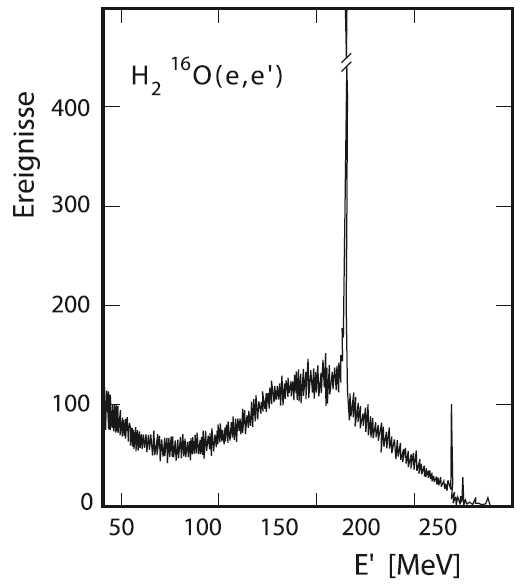
\includegraphics[width=0.5\linewidth]{img/povh_6_5.png}
    \caption{Energiespektrum von Elektronen, die an einem $\text{H}_2$O-Target gestreut wurden. 
    Die Daten wurden am Linearbeschleuniger MAMI-A in Mainz bei $\SI{246}{MeV}$ Strahlenergie unter einem Streuwinkel von $\SI{148.50}{\degree}$ aufgenommen.
    Deutlich erkennbar ist der Peak der elastischen Streuung an den quasi-freien Protonen in Wasserstoff bei $E' = \SI{160}{MeV}$. 
    Die Peaks rechts davon gehören zur elastischen Streuung am gesamten Sauerstoff-Kern. 
    Die breite Gauss-Verteilung entspricht der quasi-elastischen Streuung an Protonen im Sauerstoff-Kern. \refimgsourcebook{Povh}{Teilchen und Kerne}{978-3642378218}{85}}
    \label{fig:povh65}
\end{figure}
% 
% TODO: Figure 6.5 aus Povh, Particles and Nulcei, chapter 6.2.
% 
\begin{fquestion}{Welche Energie steht an der $x$-Achse?}
    Die Energie der gestreuten Elektronen, also $E' = \frac{E}{1 + \frac{E}{M}(1-\cos \theta)}$ (entspricht Compton-Streuung, Masse der Elektronen ist bei $E\sim \SI{100}{MeV}$ vernachlässigbar).
\end{fquestion}

\begin{fquestion}{Wo sieht man die initiale Energie der Elektronen?}
    Entspricht etwa der maximal gemessenen Energie eines gestreuten Elektrons, also ganz rechts auf der $x$-Achse.
    Üblicherweise ist $E \approx \SI{250}{MeV}$.
\end{fquestion}

\begin{fquestion}{Was für Peaks gibt es?}
    Die Bindungsenergien von H-Atomen in $\mathrm{H}_2 \mathrm{O}$ ist in der Größenordnung von eV, also gegenüber $E$ vernachlässigbar. 
    Die Elektronen streuen daher elastisch an den zugehörigen Protonen, und es gibt einen scharfen Peak bei der entsprechenden Energie $E'$. 
    Die Position ist abhängig von $\theta$ und $\frac{E}{M}$, wobei die Masse hier $M=m_p$.
    \\
    Es gibt einen weiteren scharfen, aber viel kleineren Peak für die Streuung am gesamten Sauerstoff-Kern. 
    Es ist $E_O' > E_H'$, da $M_O \approx 16m_p > m_p = M_H$.
    Der Peak liegt also deutlich weiter rechts.
    \\
    Zuletzt gibt es noch einen breiten Peak, der zur quasi-elastischen Streuung von Elektronen an Protonen im Sauerstoff-Kern gehört.
    Der Abstand des gauss-förmigen Peaks zum scharfen Peak des freien Wasserstoffs entspricht dabei gerade der Bindungsenergie $E_B$ der Protonen.
\end{fquestion}

\begin{fquestion}{Warum ist der quasi-elastische Peak so breit?}
    % Herauslösen von Protonen aus verschiedenen Energieniveaus im Kern ??? 
    Die relativ große Standardabweichung hängt mit dem großen Fermi-Impuls der Protonen über $\sigma_{\Delta E} = \frac{|\Vec{q}| p_F}{ M\sqrt{5}}$ zusammen.
    Insbesondere ist dafür die zufällige Richtung der Impulse relevant.
    Man kann $|\Vec{q}|$ über $E_\mathrm{elastisch}' = \frac{q^2}{2m_p}$ abschätzen, was gerade der Position des Wasserstoff-Peaks entspricht.
\end{fquestion}

\begin{fquestion}{Welchen interessanten Parameter des Kastenpotentials kann man dann abschätzen?}
    Aus dem Fermi-Impuls erhält man wie üblich auch die Fermi-Energie.
    Die Tiefe des Potentialkastens ist dann $V_0 = E_B + E_F$.
\end{fquestion}

% \begin{question}{Welche Energie muss dabei überwunden werden?}
%     Bindungsenergie zwischen den Nukleonen
% \end{question}

\begin{fquestion}{Wenn zwei Teilchen mit vergleichbarem Impuls elastisch stoßen, ist dann die Energie bei entgegengesetztem Impuls höher?}
    % Ja, weil größerer Relativ-Impuls und damit größerer $S$-Faktor ???
    Ja, weil der Relativ-Impuls dann größer ist, und dieser direkt in die Schwerpunktsenergie eingeht.
    Diese ist $\sqrt{s}$, wobei $s$ eine der drei Mandelstam-Variablen ist.
    Es gilt
    $$s = (p_1 + p_2)^2 = p_1^2 + p_2^2 + 2p_1\cdot p_2 = m_1^2 + m_2^2 + 2(E_1E_2 - \Vec{p}_1\cdot\Vec{p}_2).$$
    Damit wird also $\sqrt{s}$ für $\theta = \pi$ maximal.
\end{fquestion}

\subsection{Neutronenstreuung}

% \begin{question}{Warum Neutronen?}
%     elektrisch neutral, aber Spin aufgrund von Unterstruktur durch Quarks
% \end{question}

\begin{table}[H]
    \centering
    \begin{tabular}{|ll|ccc|}
        \hline
        Regime & Energie & & & \\
        \hline
        Kalt & $< \SI{1}{\milli\electronvolt}$ & \textcolor{red}{Beugung} & \textcolor{blue}{Elastisch} & \textcolor{Dandelion}{Einfang} \\
        Thermisch & $< \SI{0.5}{\electronvolt}$ & \textcolor{violet}{Kernspaltung} & \textcolor{blue}{Elastisch} & \textcolor{Dandelion}{Einfang} \\
        Epithermisch & $< \SI{50}{\kilo\electronvolt}$ & \textcolor{violet}{Kernspaltung} & \textcolor{blue}{Elastisch} & \textcolor{Dandelion}{Einfang} \\
        Schnell & $> \SI{50}{\kilo\electronvolt}$ & \textcolor{violet}{Kernspaltung} & \textcolor{blue}{Elastisch} & \textcolor{Dandelion}{Einfang} \\
        Medium & $> \SI{1}{\mega\electronvolt}$ &   & \textcolor{blue}{Elastisch} & \textcolor{Turquoise}{Inelastisch} \\
        Hochenergetisch & $> \SI{10}{\mega\electronvolt}$ &   & \textcolor{blue}{Elastisch} & \textcolor{Turquoise}{Inelastisch} \\
        \hline
    \end{tabular}
    \caption{Dominierende Wechselwirkungen (Beugung, Elastische Streuung sowie die nuklearen Reaktionen (Radioaktiver Einfang $(n, \gamma)$, andere Einfänge $(n, p)$ oder $(n, \alpha)$, Inelastische Streuung $(n, x)$ und Kernspaltung $(n, f)$) für Neutronen in verschiedenen Regimen.}
\end{table}

\begin{fquestion}{Was ist quasi-elastische Neutronenstreuung?}
    In der Festkörperphysik nutzt man die Methode der quasi-elastischen Neutronenstreuung (QENS), um Mittels kleiner Energieüberträge (unter $\si{\micro\electronvolt}$ Spektroskopie in der Größenordnung zwischen $1\ldots\SI{500}{\angstrom}$ zu studieren.
    
    Möglicherweise können im Rahmen der Teilchenphysik bei Energien um $6\ldots\SI{8}{MeV}$ die gebundenen Nukleonen beobachtet werden (Als Analogie zur quasi-elastischen Elektronenstreuung, Informationen sind hier schwer zu finden).
\end{fquestion}

\begin{fquestion}{Wie können Neutronen technisch erzeugt werden?}
    Abhängig vom gewünschten Energiebereich entweder durch Spallationsquellen (höhere Ausbeute für $E < \SI{0.1}{\mega\electronvolt}$ und $E>\SI{10}{\mega\electronvolt}$) oder Kernspaltung.
\end{fquestion}

\begin{fquestion}{Wie können Neutronen nachgewiesen werden?}
    Durch ${}^3\text{He}$- oder $\text{BF}_3$-Proportionalzählrohre mit der Reaktion ${}^3\text{He} + n \rightarrow {}^3\text{H} + p + \SI{0.764}{\mega\electronvolt}$.
    Alternativ mit Lithium-basierten Kristalldetektoren.
\end{fquestion}

\begin{fquestion}{Was ist der Vorteil von Neutronen für Streuprozesse?}
    Sie sind elektrisch neutral, können aber über ihr magnetisches Moment mit magnetischen und elektrischen Feldern wechselwirken.
    
    Außerdem ermöglicht die Dispersionsrelation der massiven Neutronen im Gegensatz zur steilen Dispersionsrelation von Photonen die Auflösung von kleinen Energien. 
\end{fquestion}

\begin{fquestion}{Wie sieht der Verlauf des Wirkungsquerschnitts von Neutronen aus?}
    Es ist $\dd \sigma \propto \frac{|p'|}{|p|} \dd \Omega$ mit den Impulsen $p$ vor und $p'$ nach der Streuung im Schwerpunktsystem.
    
    Für elastische Streuung ist $|p'| = |p|$ und entsprechend $\sigma = \mathrm{const.}$; für inelastische Streuung ist näherungsweise $|p'| = \mathrm{const.}$ (nach dem Einfang finden Kernprozesse statt, die wohldefiniert sind), entsprechend ist $\sigma \propto |p|^{-1} \propto E^{-1/2}$.
    
    \begin{center}
        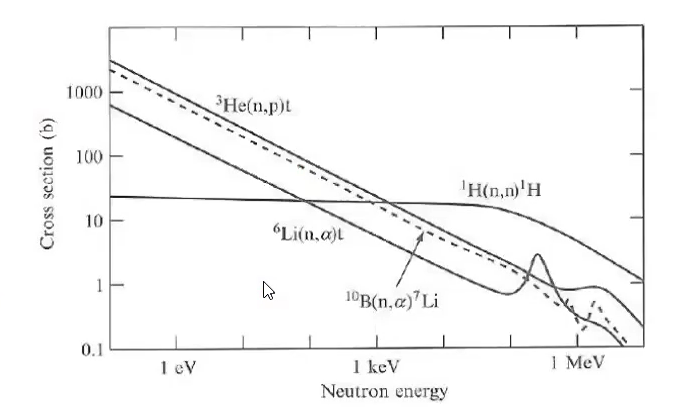
\includegraphics[width=.8\linewidth]{img/Crosssection_Neutron.png}
    \end{center}
\end{fquestion}

% \begin{question}{Wofür verwendet man Neutronenstreuung noch?}
%     Anregung von Magnonen, hier Energie nur in Größenordnung von meV
% \end{question}

\begin{fquestion}{Warum braucht man thermische Neutronen zur Strukturauflösung in Festkörpern?}
    Aus der de-Broglie Gleichung ergibt sich 
    $$E_{\mathrm{kin}} = \frac{h^2}{2 m_{\mathrm{N}} \lambda^2} \approx \SI{20}{meV}$$
    für Neutronen mit einer Wellenlänge von $\SI{200}{pm}$, was in der Größenordnung von metallischen Gitterkonstanten $\approx \SI{400}{pm}$ liegt und damit durch Interferenz deren Struktur auflösen kann. 
\end{fquestion}


% \begin{question}{Was verwendet man üblicherweise?}
%     auch Neutronen
%     besser als Röntgenstrahlung, weil benachbare Elemente unterscheidbar, leichte Elemente auflösbar ???
%     Neutronen haben große freie Weglänge und sind zerstörungsfrei, also für große Proben geeignet
%     Effekte wie Antiferromagnetismus messbar ??? 
% \end{question}


\subsection{Rutherfordstreuung}

\begin{fquestion}{Was wollte Rutherford ursprünglich messen?}
    Rutherford untersuchte die Streuung von geladenen $\alpha$-Teilchen $\mathrm{He}^{2+}$ an Goldfolie.
    
    Zur Zeit des Experiments ging man vom Thompson'schen (bzw. Plum-Pudding) Atommodell aus, bei dem Elektronen und Protonen zusammen im Atomkern vermischt das Atom bilden.
    Dieses sollte durch den Streuversuch getestet werden.
    
    Tatsächlich stellte sich heraus, dass ein großer Teil der Projektile die Folie passierte und etwa jedes einhundertausendste reflektiert wurde, was mit dem Plum-Pudding Modell nicht zu erklären war.
\end{fquestion}

\begin{fquestion}{Wie sieht der Wirkungsquerschnitt aus?}
    Der Wirkungsquerschnitt bei Streuung an einer Punktladung unter der Coloumb-Wechselwirkung ist durch 
    $$\frac{\dd \sigma}{\dd \Omega} = \left( \frac{1}{4 \pi \varepsilon_0} \frac{Z_1 Z_2 e^2}{4 E_0}\right)^2 \frac{1}{\sin^4 \theta/2}$$
    gegeben. Hier sind $Z_1$ und $Z_2$ die Ladungszahlen der beiden Streupartner und $E_0$ die kinetische Energie des einfallenden Teilchens.
    Durch die Energieabhängigkeit ist $\sigma \propto E^{-2} \propto q^{-4}$.
    
    Bei höheren Auflösungen ist die Struktur des Kerns relevant, die zu einem zusätzlichen Faktor (dem Formfaktor) führt:
    $$\frac{\dd \sigma}{\dd \Omega}  = \left(\frac{\dd \sigma}{\dd \Omega} \right)_{\mathrm{Rutherford}} |F(q^2)|^2.$$
    
    Für eine homogen geladene Kugel mit Radius $R$ und Dichte $\rho_0$ ist in natürlichen Einheiten
    $$F(q^2) = \frac{4\pi \rho_0}{q^3} (\sin q R - q R \cos q R).$$
    Entsprechend lässt sich aus dem ersten Minimum die dimensionslose Größe $R q_{\mathrm{min}} = 2 R p \sin \theta/2 = 2 R E_0 \sin \theta/2$ ablesen. 
    Der Kernradius folgt dann aus dem Vergleich mit der ersten Nullstelle des Formfaktors bei $q R \approx 4.5$.

    \begin{center}
        Verlauf des Formfaktors einer homogen geladenen Kugel
        
        \begin{tikzpicture}
            \begin{axis}[
                xmin=0, xmax=14,
                ymin=-0.05, ymax=0.35, 
                xlabel={$qR$}, ylabel={$F(q^2) / \text{abt. units}$}, 
                % ytick distance = 0.5,
                grid=both]
                \addplot[domain = 1:14,smooth,samples=500, thick] {(sin(deg(x))- x * cos(deg(x))) / (x^3)};
                \addplot[domain = 0:1,smooth,samples=50, thick] {1/3 - x^2*4/5! + x^4*6/7! - x^6*8/9!};
            \end{axis}
        \end{tikzpicture}
    \end{center}    
\end{fquestion}

\begin{fquestion}{Was ist der Formfaktor $F(q^2)$?}
    Der Formfaktor
    $$F(q^2) = \int \rho(x) \e^{\i q x} \dd x$$
    ist die Fouriertransformierte der Ladungsverteilung.
    
    Dieser entsteht phänomenologisch aus folgender Überlegung: Vor und nach einem Streuprozess ist das Elektron ein freies Teilchen, entsprechend eine ebene Welle.
    Man macht den Ansatz einer ebenen einlaufenden und kugelförmigen auslaufenden Welle 
    $$\psi = \e^{ \i \vec{k} \cdot\vec{r} } + \frac{\e^{\i kr}}{r} f(\theta, \phi).$$
    Diese wird durch die Schrödingergleichung beschrieben, man findet 
    $$\frac{\dd \sigma}{\dd \Omega} = |f|^2.$$
    In der Born'schen Näherung ergibt sich dann schließlich die obige Form für Wirkungsquerschnitt und Strukturfaktor; intuitiv kann man sich das Auftreten der Minima also als destruktive Überlagerung verschiedener Streuungen vorstellen.
\end{fquestion}

% \begin{question}{Woher kommt die Form?}
%     mathematisch aus dem Formfaktor
%     anschaulich aus der Streuung von Neutronen an mehreren Nukleonen, also Interferenzen wie beim Doppelspalt ??? 
% \end{question}

% \begin{question}{Was ist der Formfaktor?}
%     FFT der Ladungsverteilung
% \end{question}

% \begin{question}{Wie bekommt man aus dem Wirkungsquerschnitt (harte, homogene Kugel) den Kernradius?}
%     das erste Minimum ist proportional zu $\frac{1}{R}$, Formfaktor ist $\frac{\sin (q)}{q}$ ??? 
% \end{question}

% \begin{question}{Was bedeutet das, wenn die Kugel sehr groß ist?}
%     Minimum verschiebt sich zu kleineren Winkeln
% \end{question}

\begin{fquestion}{Wie hängt der Wirkungsquerschnitt vom Kugelradius ab?}
    Das Produkt $q R \propto R \sin \frac{\theta}{2}$ ist für das erste Minima konstant.
    Entsprechend würde für größere Radien $R$ der Winkel $\theta$ kleiner und für kleinere Radien der Winkel $\theta$ größer werden.
    
    Anschaulich folgt dies aus der Unschärfe der Fouriertransformation.
    % \textcolor{red}{Anschaulich folgt dies aus der Unschärfe der Fouriertransformation.}
\end{fquestion}

% \begin{question}{Wie sieht das dann für das ursprüngliche Rutherford-Modell aus?}
%     Punktladung, $R$ gegen 0, also Minimum gegen unendlich, also Formfaktor konstant (mathematisch offensichtlich, da FFT von Dirac-Delta)
% \end{question}

\begin{fquestion}{Wie sieht die Ladungsdichteverteilung eines echten Kerns aus?}
    Bei großen Kernen ist die Näherung über eine homogene Ladungsdichte gerechtfertigt, in der Realität tritt noch ein diffuser Rand in der Ordnung $\SI{2.4}{fm}$ auf (zum Vergleich: $R = R_0 A^{1/3}$ mit $R_0 = \SI{1.25}{fm}$). 
    
    Bei kleineren Kernen (${}^4\mathrm{He}$, ${}^6\mathrm{Li}$ oder ${}^9\mathrm{Be}$) ist eine gauß-förmige Näherung eher gerechtfertigt, mit ebenfalls gauß-förmigem Formfaktor.
    
    Siehe \autoref{fig:ladungstraegerdichte formfaktor} für eine Visualisierung.
\end{fquestion}

\begin{fquestion}{Was ist der Mott-Formfaktor?}
    Beim Mott-Formfaktor 
    $$\left(\frac{\dd \sigma}{\dd \Omega}\right)_{\mathrm{Mott}} = \left(\frac{\dd \sigma}{\dd \Omega}\right)_{\mathrm{Rutherford}} (1 - \beta^2 \sin^2 \theta / 2) \xrightarrow[\beta = 1]{} \left(\frac{\dd \sigma}{\dd \Omega}\right)_{\mathrm{Rutherford}} \cos^2 \theta / 2 $$
    wird zusätzlich der Spin des Elektrons berücksichtigt.
    
    Für hohe Energien muss man ebenfalls den Targetrückstoß berücksichtigen, durch welchen ein zusätzlicher Faktor
    $$\left(\frac{\dd \sigma}{\dd \Omega}\right)_{\mathrm{Mott}} = \left(\frac{\dd \sigma}{\dd \Omega}\right)_{\mathrm{Mott}}^* \frac{E'}{E}$$
    durch ein sich änderndes Phasenraumvolumen eingeführt wird.
\end{fquestion}

% \begin{question}{Wie sieht das bei größeren Kernen aus?}
%     Radius wird größer, aber Ladungsdichte bleibt gleich
% \end{question}

% \begin{question}{Wie kann man das Auftreten der Minima erklären?}
%     Elektron streut als eben Welle am kern, Überlagerung der gestreuten Wellenfronten von verschiedenen Stellen des Kerns erzeugt destruktive Interferenz
% \end{question}

\subsection{Elektronenstreuung am Kern}

\begin{table}[H]
    \centering
    \begin{tabular}{m{4cm}>{\centering}m{3cm}>{\centering}m{3cm}m{4cm}}
        & $\rho(r)$ & $F(q^2)$ & \\
        $\rho(r) = \frac{\delta(r)}{4\pi}$ & \begin{tikzpicture}
\pgfplotsset{%
    width=4.9cm,
    height=3.5cm
}
            \begin{axis}[domain=0:1, xmin=0, xmax=1, ymin=0, ymax=1.1, ticks = none]
                \draw[-, line width=1mm, black] (axis cs:0,0) -- (axis cs:0,1);
                \node[] at (axis cs: .5,.5) {\normalsize
 punktförmig};
            \end{axis}
        \end{tikzpicture}
 & \begin{tikzpicture}
\pgfplotsset{%
    width=4.9cm,
    height=3.5cm
}
            \begin{axis}[domain=0:1, xmin=0, xmax=1, ymin=0, ymax=1.1, ticks = none]
                \addplot [thick, black, samples=50] {1};
                \node[] at (axis cs: .5,.5) {\normalsize
 konstant};
            \end{axis}
        \end{tikzpicture} & $F(q^2)=1$ \\
    $\rho(r) = \frac{a^3}{8\pi} e^{-a r}$ &  \begin{tikzpicture}
\pgfplotsset{%
    width=4.9cm,
    height=3.5cm
}
            \begin{axis}[domain=0:1, xmin=0, xmax=1, ymin=0, ymax=1.1, ticks = none]
                \addplot [thick, black, samples=50] {exp(-2*x)};
                \node[] at (axis cs: .5,.5) {\normalsize
 exponentiell};
            \end{axis}
        \end{tikzpicture} &  \begin{tikzpicture}
\pgfplotsset{%
    width=4.9cm,
    height=3.5cm
}
            \begin{axis}[domain=0:1, xmin=0, xmax=1, ymin=0, ymax=1.1, ticks = none]
                \addplot [thick, black, samples=50] {(1 + 4 * x^2)^(-2)};
                \node[] at (axis cs: .5,.5) {\normalsize
 Dipol};
            \end{axis}
        \end{tikzpicture} & $F(q^2) = \left(1 + \frac{q^2}{a^2 \hbar^2}\right)^{-2}$ \\
    $\rho(r) = \sqrt[3]{\frac{a^2}{2\pi}} e^{-\frac{a^2 r^2}{2}}$ & \begin{tikzpicture}
\pgfplotsset{%
    width=4.9cm,
    height=3.5cm
}
            \begin{axis}[domain=0:1, xmin=0, xmax=1, ymin=0, ymax=1.1, ticks = none]
                \addplot [thick, black, samples=50] {exp(-4*x^2)};
                \node[] at (axis cs: .5,.5) {\normalsize
 gaußförmig};
            \end{axis}
        \end{tikzpicture} & \begin{tikzpicture}
\pgfplotsset{%
    width=4.9cm,
    height=3.5cm
}
            \begin{axis}[domain=0:1, xmin=0, xmax=1, ymin=0, ymax=1.1, ticks = none]
                \addplot [thick, black, samples=50] {exp(-4*x^2)};
                \node[] at (axis cs: .5,.5) {\normalsize
 gaußförmig};
            \end{axis}
        \end{tikzpicture} & $F(q^2) = e^{-\frac{q^2}{2 a^2 \hbar^2}}$ \\
    $\rho(r) = \begin{cases} \frac{3}{4 \pi R^3} & r\leq R \\ 0 & r > R \end{cases}$ & \begin{tikzpicture}
\pgfplotsset{%
    width=4.9cm,
    height=3.5cm
}
            \begin{axis}[domain=0:1, xmin=0, xmax=1, ymin=0, ymax=1.1, ticks = none]
                \addplot [thick, black, samples=100] {1/(1+exp((x-0.5)/0.00001))};
                \node[] at (axis cs: .5,.5) {\normalsize
 Homogene Kugel};
            \end{axis}
        \end{tikzpicture} & \begin{tikzpicture}
\pgfplotsset{%
    width=4.9cm,
    height=3.5cm
}
            \begin{axis}[domain=0:10, xmin=0, xmax=10, ymin=0, ymax=0.4, ticks = none]
                \addplot[domain = 1:10,smooth,samples=500, thick] {abs((sin(deg(x))- x * cos(deg(x))) / (x^3))};
                \addplot[domain = 0:1,smooth,samples=50, thick] {1/3 - x^2*4/5! + x^4*6/7! - x^6*8/9!};
                \node[] at (axis cs: 5,.2) {\normalsize
 oszillierend};
            \end{axis}
        \end{tikzpicture} & $F(q^2) = \frac{3(\sin x - x \cos x)}{x^3}$, wobei $x = |q|R / \hbar$\\
    $\rho(r) = \frac{\rho_0}{1 + e^{\frac{r - c}{a}}}$ & \begin{tikzpicture}
\pgfplotsset{%
    width=4.9cm,
    height=3.5cm
}
            \begin{axis}[domain=0:1, xmin=0, xmax=1, ymin=0, ymax=1.1, ticks = none]
                \addplot [thick, black, samples=50] {1/(1+exp((x-0.5)/0.04))};
                \node[] at (axis cs: .5,.5) {Diffuse Kugel};
            \end{axis}
        \end{tikzpicture} & \begin{tikzpicture}
\pgfplotsset{%
    width=4.9cm,
    height=3.5cm
}
            \begin{axis}[domain=0:10, xmin=0, xmax=10, ymin=0, ymax=0.4, ticks = none]
                \addplot[domain = 1:10,smooth,samples=500, thick] {abs((sin(deg(x))- x * cos(deg(x))) / (x^3))};
                \addplot[domain = 0:1,smooth,samples=50, thick] {1/3 - x^2*4/5! + x^4*6/7! - x^6*8/9!};
                \node[] at (axis cs: 5,.2) {\normalsize
 oszillierend};
            \end{axis}
        \end{tikzpicture} & Keine analytische Form
        \\
        & $r \rightarrow \infty$ & $q \rightarrow \infty$ &
    \end{tabular}
    \caption{Gegenüberstellung verschiedener Ladungsträgerdichten $\rho(r)$ und ihrer Formfaktoren $F(q^2)$.}
    \label{fig:ladungstraegerdichte formfaktor}
\end{table}

% (Streuquerschnitt für eine diffuse Kugel)

% \begin{question}{Wo sieht man den Kernabstand?}
%     Das erste Minimum des Formfaktors $F(q^2)$ ist proportional zu $\frac{1}{r_0}$.
% \end{question}

% \begin{question}{Kann bei Auflösung mehrerer Teilchen mehr Energie haben, als bei einem einzelnen?}
%     nein, die Streuung an einem Teilchen (z.B. Punktladung) gibt Maxima
%     die Streuung an vielen Nukleonen bringt durch Überlagerung nur (kleinere) Nebenmaxima und zusätzliche Minima (vergleiche Interferenzmuster von $N$ Spalten in Optik).
% \end{question}

\begin{fquestion}{Was passiert bei der Elektron-Kern-Streuung bei höheren Energien?}
    Nach den elastischen Stoßprozessen kommen zunächst die \textit{inelastischen Kernanregungen}, dort werden bei einigen $\SI{10}{MeV}$ Riesendipolresonanzen und Übergänge zwischen Kernzuständen angeregt.
    
    Danach finden elastische Stoßprozesse an den einzelnen Nukleonen bei Energien von $\SI{0.2}{GeV}\ldots\SI{10}{GeV}$ statt, durch welche die elektrischen und magnetischen Eigenschaften von Proton und Neutron untersucht werden können. 
    Man beobachtet, dass das Proton einen Dipolformfaktor entsprechend einer exponentiellen Ladungsverteilung aufweist.
    
    In diesem Energiebereich kann man bei größeren Kernen (Beispiel: $\text{H}_2$O) über \textit{quasi-elastische Streuung} (Wechselwirkung mit nur einem Nukleon im Kern, welches danach aus dem Verband gelöst ist) die Tiefe des Kernpotentials ($17\ldots\SI{44}{MeV}$, aus der Verschiebung zur elastischen Streuung) sowie den Fermi-Impuls ($170 \ldots \SI{270}{MeV/c}$, aus der Breite der Verteilung) bestimmen.
    
    Bei noch größeren Energie von einigen $\SI{100}{GeV}$ kommt es zu \textit{tiefinelatischen Stößen}, bei denen die Unterstruktur (Quarks) der Nukleonen aufgelöst werden können.
    Hier beobachtet man beispielsweise die $\Delta^+$-Resonanz des Protons bei einer Masse von $W=\SI{1232}{MeV}$ ($|\Delta^+\rangle = |\mathrm{u}^\uparrow \mathrm{u}^\uparrow \mathrm{d}^\uparrow \rangle$, siehe auch Povh, 16.2 Baryonenmultipletts).
    
    Misst man die Strukturfunktionen, kann man außerdem bestimmen dass der Wirkungsquerschnitt unabhängig von $q^2$ ist, man also an punktförmigen Teilchen streut und die Konstituenten des Protons den Spin $1/2$ tragen müssen.
\end{fquestion}

% \begin{question}{Was passiert bei noch höheren Elektronenergien?}

%     Man kann die Ladungsverteilung der Protonen im Kern auflösen.
%     Anhand der gemessenen Formfaktoren kann man auf die Struktur des Nukleons schließen.
%     % Formfaktoren, kann aus Streubildern auf die Verteilung des Streutargets schließen
% \end{question}

% \begin{question}{Was passiert bei noch höheren Energien?}
%     Auflösung der Quark-Struktur der Protonen bzw. Quarkanregungen (bspw. $\Delta^+$-Resonanz, also $|\mathrm{u}_\uparrow \mathrm{u}_\uparrow \mathrm{d}_\uparrow \rangle$ mit Spin 3/2.)
% \end{question}

\begin{fquestion}{Welche Anregungen kann man bei Quarks beobachten?}
    Bei Quarks wurden bisher keine Anregungen gefunden, weshalb man davon ausgeht, dass es sich um fundamentale Teilchen ohne Unterstruktur handelt.
    
    Bei Nukleonen kann man hingegen Spin-Anregungen wie die Delta-Resonanzen beobachten.
    Möglich sind auch Anregungen im Kern.
\end{fquestion}

\begin{fquestion}{Wie viele Größen braucht man, um Streuung zu beschreiben?}
    Für die elastische Streuung benötigt man einen Parameter (etwa den Streuwinkel $\theta$).
    
    Bei der inelastischen Streuung benötigt man zusätzlich einen weiteren Parameter, beliebte Paare sind etwa $(E', \theta)$, $(q^2, \nu)$ oder $(q^2, x)$.
    Hier ist 
    $$\nu \equiv \frac{Pq}{M} \xrightarrow[\text{Labor}]{} E - E'$$
    ein Maß für den Energieübertrag und die Bjorken'sche Skalenvariable
    $$x = \frac{q^2}{2 M \nu}$$
    ein Maß für die Inelastizität des Prozesses.
    Bei $x=1$ ist der Prozess vollkommen elastisch, für $0 < x < 1$ entsprechend inelastisch.
\end{fquestion}

\begin{fquestion}{Was ist die anschauliche Bedeutung der Bjorken'schen Skalenvariable bei hohen Energien?}
    In der Stoßnäherung (quasi-elastisch: Wechselwirkung mit den individuellen Partonen) gibt $x$ den Anteil eines einzelnen Partons (bei vernachlässigbarer Ruhemasse) am Gesamtimpuls des Nukleons an.
\end{fquestion}

\cleardoublepage
\section{Kollektive Anregungen}
\addcontentsline{qst}{section}{\thesection \hspace{.5em} Kollektive Anregungen}
% \begin{question}{Warum kommt es zu Riesenresonanzen oder Plasmonen? Eine Spinwelle oder ein Phonon sind doch auch eine kollektive Anregung, trotzdem gibt es hier keinen Sprung in den Energieskalen?}
%     Resonanz ist das Stichwort, 'peaks' jeglicher Art sind dafür typisch
%     Phononen und Spinwellen sind wie Photonen, bei denen gibt es ja auch nicht grundsätzlich einen Sprung in der Anregungsenergie, außer eben bei Plasmonen
% \end{question}

\begin{fquestion}{Was sind die relevanten Größenordnungen bei Dipolriesenresonanzen (GDR) und Oberflächenplasmonen (SPR)?}
   GDR: $E\approx (7\dots 40)\,$MeV, beruht auf starker Wechselwirkung (Kernkraft, Oberflächenterme), Anregung durch Photonen und Neutronen %(auch durch Elektronen mit $E\gtrsim 50\,$MeV über eine Art umgekehrter innerer Konversion ??? )
   \\
   SPR: $E\sim 1\,$eV (optisches Spektrum, $\omega \simeq \omega_\mathrm{plasma}$ !), beruht auf elektromagnetischer Wechselwirkung (Coulomb, Polarisation), Anregung durch Photonen
\end{fquestion}

\subsection{Plasmonen}

\begin{fquestion}{Was sind Plasmonen?}
    Plasmonen sind quantisierte Schwingungen der Elektronendichte. 
    Sie sind somit eine kollektive Schwingungsanregung von Elektronen. 
    Die Dispersionsrelation von Oberflächenplasmonen
    \[\omega = \omega_p \sqrt{1 + \frac{c^2k^2}{\varepsilon(\infty)}}.\]
    
    \begin{center}
        \begin{tikzpicture}
            \centering
            \begin{axis}[domain=0:3, xmin=0, xmax=3, ymin=0, xlabel = {$k c / \sqrt{\varepsilon(\infty)}$}, ylabel = {$\omega / \omega_p$}]
                \draw[red, fill = red!30!white] (0,0) rectangle (3,1) node[pos=.5] {Verbotene Frequenzlücke};
                \addplot [thick, black, samples=50] {sqrt(1 + x^2)};
            \end{axis}
        \end{tikzpicture}
    \end{center}
\end{fquestion}

% \begin{fquestion}{Wodurch werden Plasmonen angeregt?}
%     Photonen
% \end{fquestion}

\begin{fquestion}{Warum nutzt man zur Anregung von Plasmonen keine Neutronen?}
    Neutronen besitzen keine äußere Ladung und können daher nur über das magnetische Moment wechselwirken.
    Diese Anregung ist schwächer als die elektromagnetische Anregung über Photonen.
\end{fquestion}

\begin{fquestion}{Von was hängt die Plasmafrequenz ab?}
    Sie ist abhängig von der Elektronendichte $n_e$ und der effektiven Masse $m^\star$ der Elektronen 
    \[\omega_p = \sqrt{\frac{n_e e^2}{m^\star \varepsilon_0}}\]
\end{fquestion}

\begin{fquestion}{Wie ist der Zusammenhang zwischen Plasmonen und den optischen Eigenschaften von Metallen?}
    Unterhalb der Plasmafrequenz können Plasmonen durch die Interaktion mit den Photonen erzeugt werden, diese werden also absorbiert (und durch Rückkopplung der Plasmonen mit der Luft entsprechend reflektiert).
    Oberhalb der Plasmafrequenz geschieht dies nicht und die Photonen werden transmittiert.
    
    Da die Plasmafrequenz bei den meisten Metallen im ultravioletten liegt, erhalten sie ihren typischen metallischen Glanz.
\end{fquestion}

% \begin{question}{Was schwingt im Zusammenhang mit Reflexion?}
%     Licht mit einer Frequenz über der Plasmafrequenz ist transmittiert, Licht mit einer Frequenz unter der Plasmafrequenz ist relfektiert. 
%     bei höherer Frequenz können die Elektronen nicht schnell genug reagieren??? (Erklärung Wikipedia, komisch)
% \end{question}

\begin{fquestion}{Wo treten Plasmonen auf?}
    In Metallen und Halbleitern. 
    In Halbleitern kann man über Dotierung die Elektronendichte steuern und somit die Plasmafrequenz und die Reflektivität einstellen.
\end{fquestion}

\subsection{Riesenresonanzen}

% \begin{question}{Durch welches Potential werden Atomkerne im Schalenmodell beschrieben?}
%     Durch das Woods-Saxon-Potential
%     \[V(r) = \frac{-V_0}{1 + \exp\left(\frac{r - R}{a}\right)}\]
%     mit Potentialtiefe $V_0 \approx \SI{40}{MeV}$, Radiusparameter $r_0 \approx \SI{1.2}{\femto\metre}$, Potentialrand $a \approx \SI{0.5}{\femto\metre}$ und Radius $R =  r_0 A^{1/3}$.
% \end{question}

\begin{fquestion}{Was sind Riesenresonanzen?}
    Riesenresonanzen sind kollektive Schwingungsanregungen von Nukleonen im Kern, invers zum $\gamma$-Zerfall. 
    Sie haben die Energien im Bereich von $10\ldots 40\, \si{\mega\electronvolt}$. 
    Sie haben hohe Energie und Wirkungsquerschnitt.  
    
    Abgeregt werden die Schwingungen durch Kernspaltung, $n$- oder $\alpha$-Emission.
\end{fquestion}

\begin{fquestion}{Was ist das Steinwedel-Jensen-Modell?}
    Das Steinwedel-Jensen-Modell erklärt Riesenresonanzen über Dichtebewegungen der Neutronen und Protonen als Fluid.
    Die Resonanz entspricht dann einer stehenden Welle mit Wellenlänge $\lambda \sim R$, wobei  $R$ der Kernradius ist.
    Insbesondere gilt dann $E_\mathrm{SJ} \sim \frac{1}{\lambda} \sim \frac{1}{A^{1/3}}$.
\end{fquestion}

\begin{fquestion}{Was ist das Goldhaber-Teller-Modell?}
    Im Goldhaber-Teller-Modell werden die Riesenresonanzen durch Schwingungen der Protonen gegen die Neutronenwolke beschrieben.
    Für die semiempirische Beschreibung ist der Oberflächenterm aus der Bethe-Weizsäcker-Formel interessant, da $E\sim \frac{(N_O - Z_O)^2}{A_O} \sim \frac{ (R^2)^2}{R^2} = R^2$ (der Index $O$ steht für die Nukleonen an der Oberfläche).
    Man kann die Schwingung dann als harmonischen Oszillator mit $E\sim R^2\Delta x^2 \overset{!}{\sim} m\omega^2\Delta x^2$ auffassen, woraus sich $E_\mathrm{GT}\sim \omega\sim \sqrt{\frac{R^2}{m}} \sim \sqrt{\frac{A^{2/3}}{A}} \sim \frac{1}{A^{1/6}}$ ergibt.
\end{fquestion}

\begin{fquestion}{Wie verändert sich die Riesenresonanz eines Isotops für verschiedene Massen?}
    Für einen kugelsymmetrischen Kern gibt es nur eine Schwingungsmode, die Resonanz beteht dann nur aus einem Peak.
    Durch Hinzufügen von Neutronen wird der Kern deformiert, wodurch es zwei unterschiedliche Moden gibt. 
    Das spiegelt sich dann in dem Aufspalten in zwei Peaks wieder (beispielsweise bei ${}^{142\dots 150}\mathrm{Nd}$).
\end{fquestion}

% \begin{question}{Wodurch werden Riesenresonanzen angeregt?}
%     Beispielsweise durch hochenergetische Neutronen, Photonen oder Elektronen. 
% \end{question}

\begin{fquestion}{Warum kann ${}^{235}\mathrm{U}$ durch Neutronen gespalten werden, ${}^{238}\mathrm{U}$ aber nicht?}
    Die Potentialbarriere bei großen Kernen ist ungefähr 6\,MeV. 
    Die Bindungsenergie der Neutronen bei ${}^{235}\mathrm{U}$ ist 6\,MeV und reicht als Aktivierungsenergie für die Kernspaltung. 
    Die Bindungsenergie der Neutronen bei ${}^{238}\mathrm{U}$ ist 4.8\,MeV und reicht nicht als Aktivierungsenergie, das Neutron müsste noch ca. 1\,MeV kinetische Energie haben.  
    
    Die Diskrepanz der Bindungsenergien kommt aus dem Paarungsterm, eine gerade Anzahl an Neutronen ist bevorzugt.
    Dabei hat ${}^{235}\mathrm{U}$ eine gerade Anzahl Neutronen, ${}^{238}\mathrm{U}$ nicht.
    
\end{fquestion}

\begin{fquestion}{Warum entstehen bei der Kernspaltung meistens ein leichter und ein schwerer Kern?}
    Kerne mit magischen Zahlen sind stabiler, ein asymmetrischer Zerfall ist daher energetisch günstiger, wenn die Tochterkerne nah an Kernen mit magischen Zahlen liegen. 
\end{fquestion}

\begin{fquestion}{Woher kommen die schweren Elemente im Universum?}
    Aus Supernovae und der Fusion von Neutronensternen.
    Dort werden bei der Fusion entstehende Elemente schnell mit Neutronen angereichert und können dann über $\beta^-$-Zerfall zu stabilen Elementen zerfallen.  
\end{fquestion}

\begin{fquestion}{Multipolstrahlung?}
    Die Paritätsänderung $\Delta P = \pm 1$ ist $\Delta P = (-1)^{\ell}$ für elektrische Übergänge $E_\ell$ und $\Delta P = -(-1)^{\ell}$ für magnetische Übergänge $M_\ell$.
    Hierbei steht $\ell = 1$ für Dipolstrahlung, $\ell = 2$ für Quadrupolstrahlung, etc.
    In der Tabelle sind diese für einige Werte aufgelistet.
    Der eingeklammerte Term entspricht jeweils der nächsthöheren Ordnung. 
    \begin{center}
    \begin{tabular}{c|c|c|c|c}
        $\Delta J$ & $0^\ast$ & 1 & 2 & 3 \\ \hline
        $\Delta P = -1$ & $E_1 (M_2)$ & $E_1 (M_2)$ & $M_2 (E_3)$ & $E_3 (M_4)$ \\
        $\Delta P = +1$ & $M_1 (E_2)$ & $M_1 (E_2)$ & $E_2 (M_3)$ & $M_3 (E_4)$ \\
    \end{tabular}
    \end{center}
    Für $\Delta J \in \{-1,0,+1\}$ gilt dann $\Delta L = \pm 1$ und $\Delta S = 0$ für elektrische Übergänge, und $\Delta L = 0$ und $\Delta S = \pm 1$ für magnetische Übergänge, damit jeweils die Paritätsänderung mit $\Delta L$ übereinstimmt.
    \\
    $0^\ast$: Der strahlungslose Übergang $0\rightarrow 0$ ist verboten.
\end{fquestion}

\begin{fquestion}{Ist der 1S Hyperfeinübergang in Wasserstoff über $E_1$-Dipolstrahlung möglich?}
    Nein, weil für einen $E_1$-Übergang $\Delta L = \pm 1$ gelten muss.
    Beim 1S-Übergang ist aber $\Delta L = 0$, womit zumindest der magnetische $M_1$-Übergang möglich ist.
    Dieser ist allerdings stark unterdrückt, da
    $$\Gamma_M \simeq \Gamma \left(\frac{p}{m_e}\right)^2 \approx \Gamma\alpha^2.$$
    Hierbei wurde $p\approx\frac{1}{r_0} = \alpha m_e$ verwendet.
    Der Faktor $\frac{p}{m_e}$ entspricht dabei näherungsweise $\frac{E_\gamma }{E_0}$ aus der theoretischen Vorhersage.
    Die klassische Abschätzung für die elektrische Dipolstrahlung ist $\Gamma = \frac{\alpha}{3} R^2E_\gamma^3 \approx \frac{E_\gamma^3}{3\alpha m_e^2}$ (mit $R\approx r_0$).
    Es gilt $E_\gamma \simeq \SI{6}{\micro eV}$, also
    $$\Gamma_M \approx \frac{\alpha E_\gamma^3}{3m_e^2} \approx \SI{2e-30}{eV}.$$
    Das entspricht einer Lebensdauer von $\tau_M = \frac{1}{\Gamma_M} \approx \SI{1e7}{a}$, was mit dem experimentellen Wert von $\SI{1.1e7}{a}$ gut übereinstimmt.
\end{fquestion}

\begin{fquestion}{In welchen Systemen kann man die elektrische Quadrupolstrahlung vernachlässigen?}
    Die Multipolentwicklung basiert auf $\e^{\i kr} \simeq 1 + \i kr + \frac{1}{2}(\i kr)^2 + \dots$, höhere Ordnungen sind also jeweils um einen Faktor $RE_\gamma$ unterdrückt.
    Für das Verhältnis von Quadrupolstrahlung ($E_2$) zu Dipolstrahlung ($E_1$) gilt dann $r := \frac{E_2}{E_1} \sim |RE_\gamma|^2$.
    \begin{center}
        \begin{tabular}{c|c|c|c}
             & $E_\gamma$ & $R$ & $r$ \\ \hline
            Atom & $\sim \SI{10}{eV}$ & $\sim \SI{0.1}{nm}$ & $\sim \frac{1}{40000}$ \\ 
            Kern & $\sim \SI{1}{MeV}$ & $\sim \SI{10}{fm}$ & $\sim \frac{1}{400}$ \\ 
            Meson & $\sim \SI{100}{MeV}$ & $\sim \SI{0.01}{MeV^{-1}}$ & $\sim 1$ \\ 
        \end{tabular}
    \end{center}
    Bei Mesonen wurde in der Tabelle die Abschätzung $R\sim \frac{1}{\alpha_s m_\mathrm{const}^\mathrm{quark}} \approx \frac{1}{0.1 \cdot \SI{1000}{MeV}}$ verwendet.
    Für Mesonen sind die höheren Momente also prinzipiell nicht vernachlässigbar.
\end{fquestion}    
% Man kann die Schwingung dann als harmonischen Oszillator mit $E\sim R^2\Delta x^2 \overset{!}{\sim} m\omega^2\Delta x^2$ auffassen, woraus sich $E_\mathrm{GT}\sim \omega\sim \sqrt{\frac{R^2}{m}} \sim \sqrt{\frac{A^{2/3}}{A}} \sim \frac{1}{A^{1/6}}$ ergibt.



\cleardoublepage
\section{Mehrelektronensysteme und Quasiteilchen}
\addcontentsline{qst}{section}{\thesection \hspace{.5em} Mehrelektronensysteme und Quasiteilchen}
\subsection{Phononen}


\begin{fquestion}{Was ist eine Dispersionsrelation?}
    Ganz grundsätzlich gibt die Dispersionsrelation eine Energie-Impuls-Beziehung wieder, etwa $E \propto f(p)$ oder $\omega \propto g(k)$.
\end{fquestion}

\begin{figure}[htb]
    \centering
    %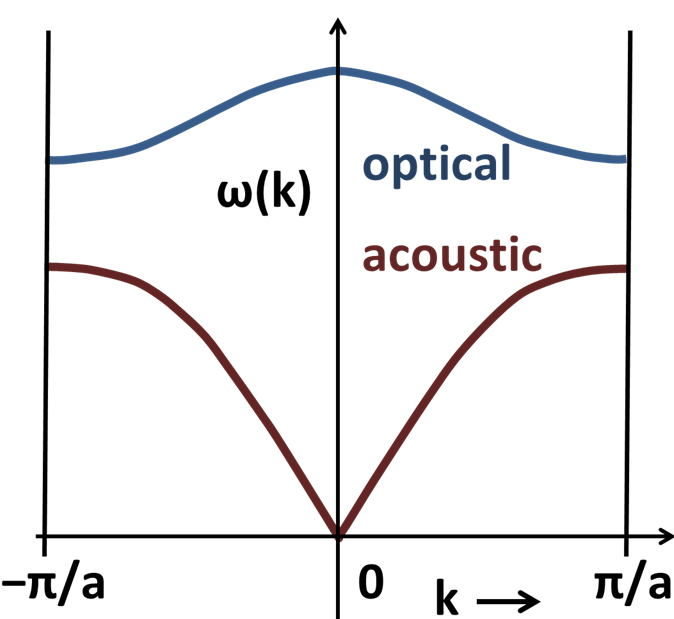
\includegraphics[scale=0.4]{img/Diatomic_phonons.png}
    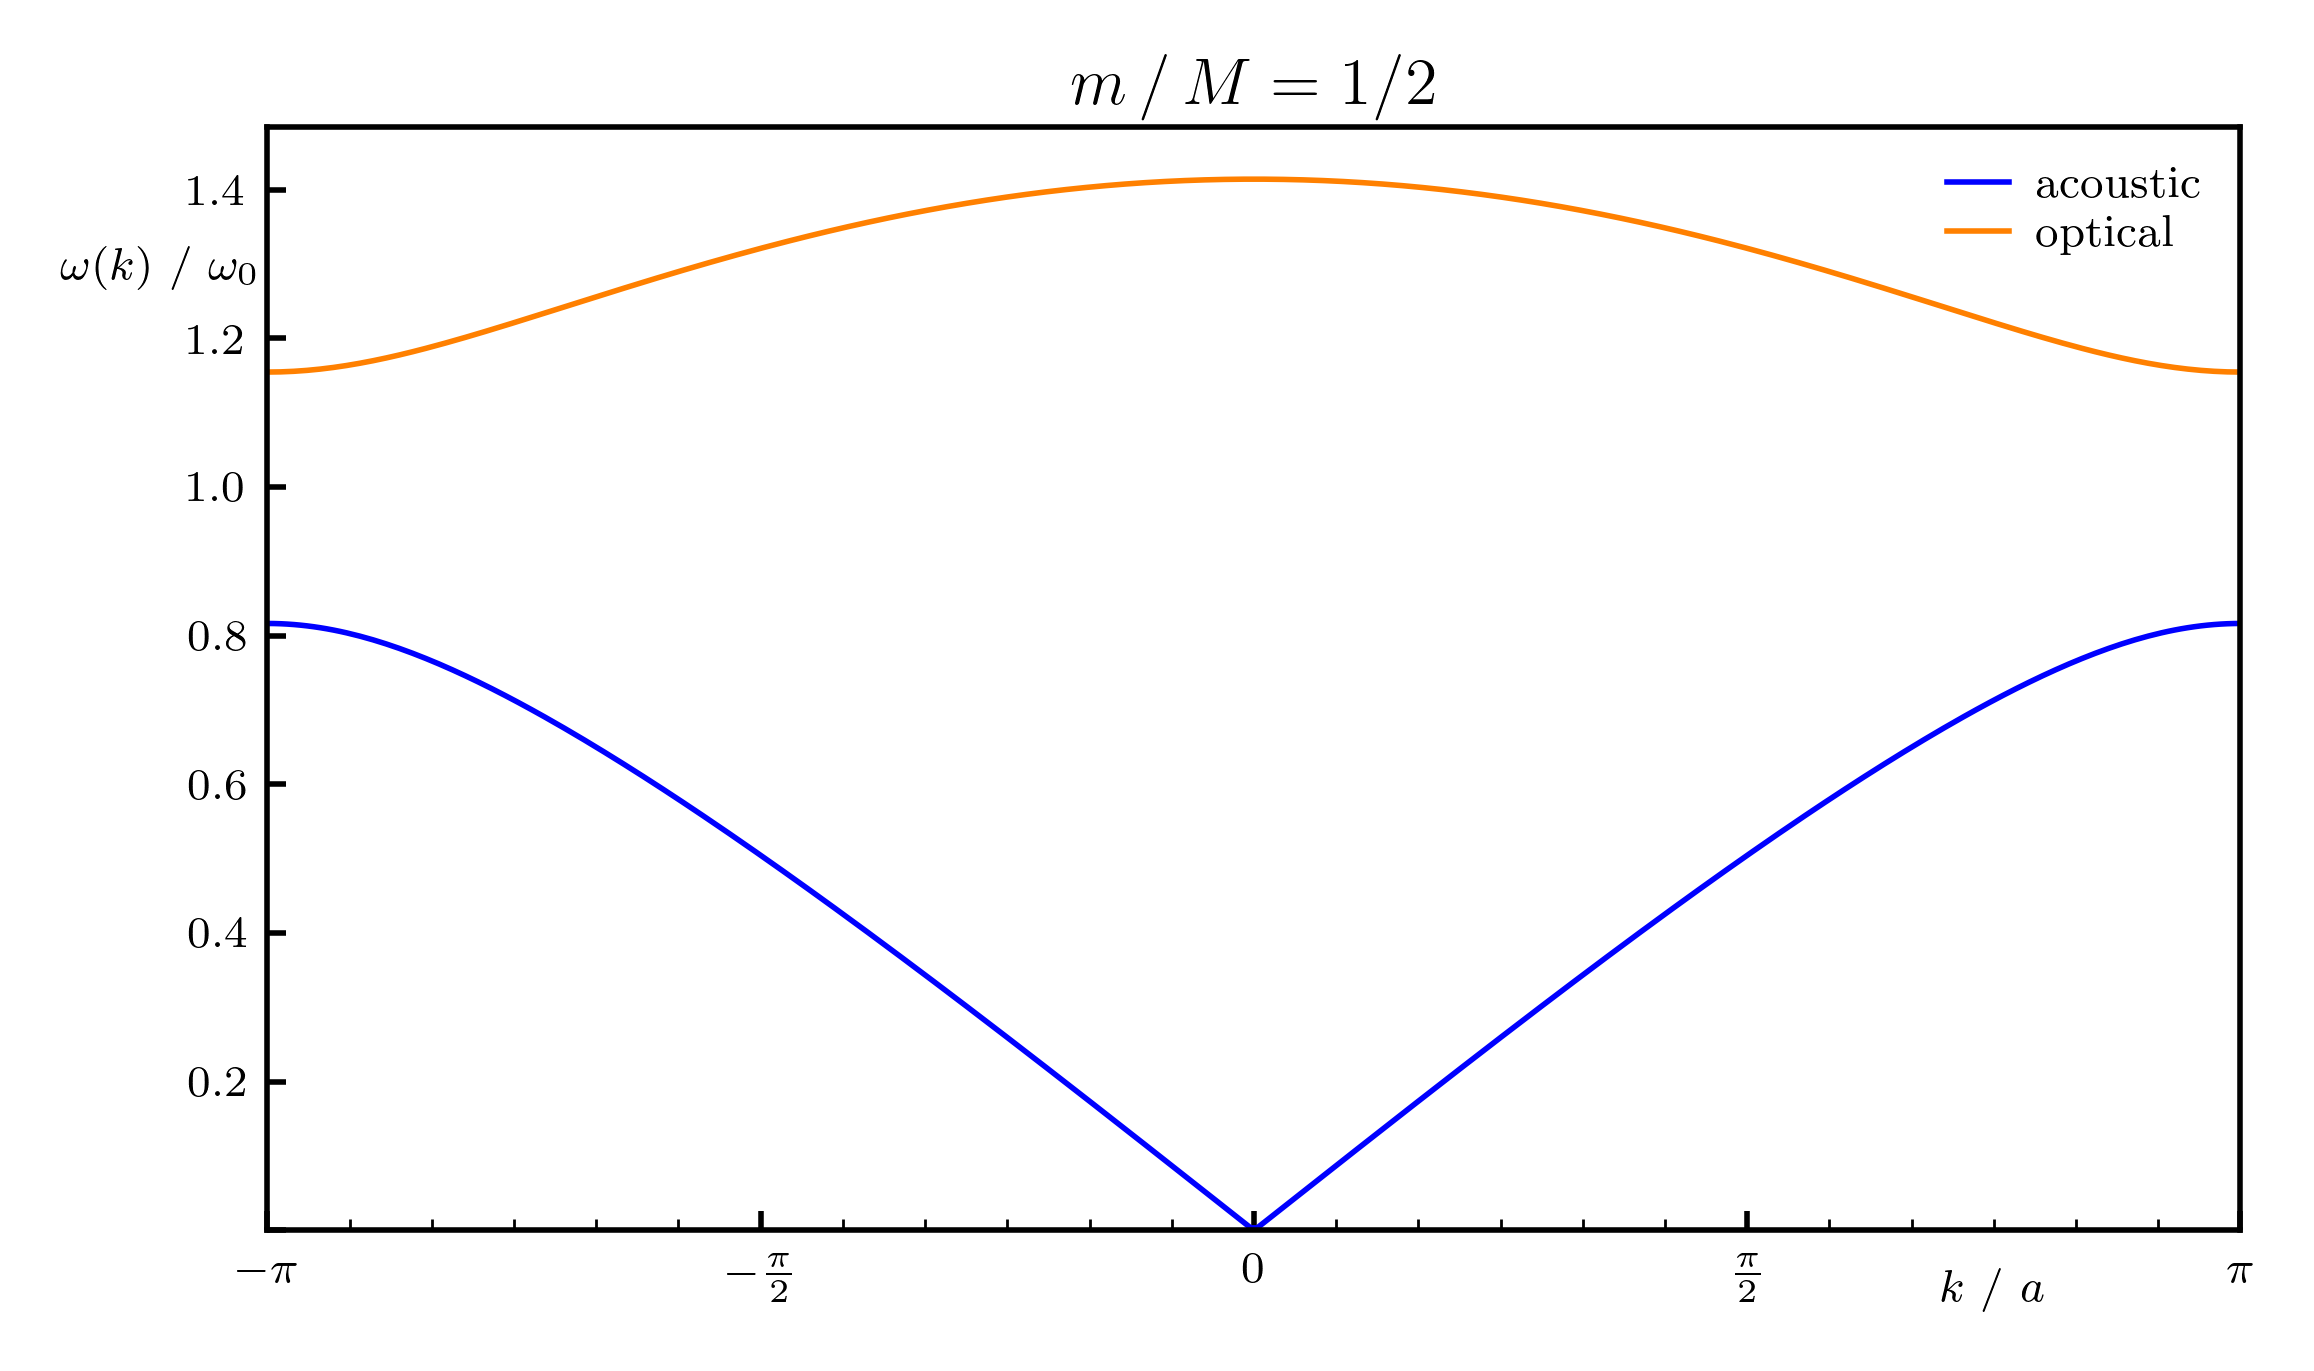
\includegraphics{img/phonon_branch2.png}
    \caption{Akustischer und optischer Zweig der Dispersionsrelation einer zweiatomigen, linearen Schwingungskette.} %\refimgsource{Wikimedia}{https://commons.wikimedia.org/wiki/File:Diatomic_phonons.png}{18.01.2022}{https://commons.wikimedia.org/wiki/File:Diatomic{\_}phonons.png}}
    \label{fig:phononen-dispersion}
\end{figure}

\begin{fquestion}{Wie ist die phononische Dispersionsrelation?}
    Mit der reduzierten Masse \( \mu = \frac{m M}{m + M} \), den Atommassen $m$ und $M$ sowie der Federkonstante $C$ und der Zellengröße $a$ ist
    \[\omega_\pm^2(k) = \frac{C}{\mu} \pm \sqrt{\frac{C^2}{\mu^2} - \frac{4 C^2}{m M} \sin^2 \left(\frac{k a}{2}\right)}. \]
    Sie ist in \autoref{fig:phononen-dispersion} dargestellt.
\end{fquestion}

% \begin{question}{Wie groß ist der Energieunterschied am Brillouin-Zonen-Rand?}
%     Vergleich zur Bandlücke, siehe Bändermodell.
%     Atome der Basis haben unterschiedliche Massen, am BZ-Rand schwingt jeweils dominant (bzw. nur) die eine oder die andere, also ist die Frequenz $\sqrt{\frac{2C}{m}}$ bzw. $\sqrt{\frac{2C}{M}}$
%     Wellenlänge der Schwingungen ist dabei gleich
%     Herleitung über lineare Kette und Vergleich zum HO ??? 
% \end{question}

\begin{fquestion}{Warum ist die Dispersion am Rand flach? }
    Die Gruppengeschwindigkeit entspricht Ableitung der Dispersionsrelation.
    Bei \(|k| = \pi/a\) bildet sich eine stehende Welle, deren Gruppengeschwindigkeit \( v_g = \frac{\partial \omega}{\partial k} = 0\) verschwindet.
    Anschaulich werden die Wellen an der nächsten Basis reflektiert und überlagern sich so zur stehenden Welle.
\end{fquestion}

\begin{fquestion}{Was ist die Debye-Frequenz $\omega_D$?}
    Die Debye-Frequenz $\omega_D = v_s \pi N / L$ ($v_s\ldots$ Schallgeschwindigkeit im Medium, $N\ldots$ Atomzahl, $L\ldots$ Systemgröße) beschreibt die größte vorkommende Phononenfrequenz.
\end{fquestion}

\begin{fquestion}{Wie kann man die Dispersionsrelation von Phononen messen?}
% https://www.quora.com/How-can-we-measure-phonons
    Üblicherweise verwendet man inelastische Neutronenstreuung.
    Inzwischen kann auch vermehrt Streuung von Röntgen-Photonen benutzt werden.  
    Die Neutronen (oder Photonen) erfahren bei der Streuung an Phononen (also quantisierten Gitterschwingungen) eine Änderung von Energie und Impuls. 
    % Die optischen Phononen haben typischerweise eine höhere Energie und können über Raman-Spektroskopie gemessen werden.
    % Für akustische Phononen kann Brillouin-Streuung 
    % Andere Methode ist EELS (electron-energy-loss-spectroscopy).
\end{fquestion}

\begin{fquestion}{Welche Größen misst man, um die Dispersionsrelation zu bestimmen?}
    Energie $E'$ und Winkel $\theta'$ der gestreuten Neutronen
\end{fquestion}

\begin{figure}[!ht]
    \centering
    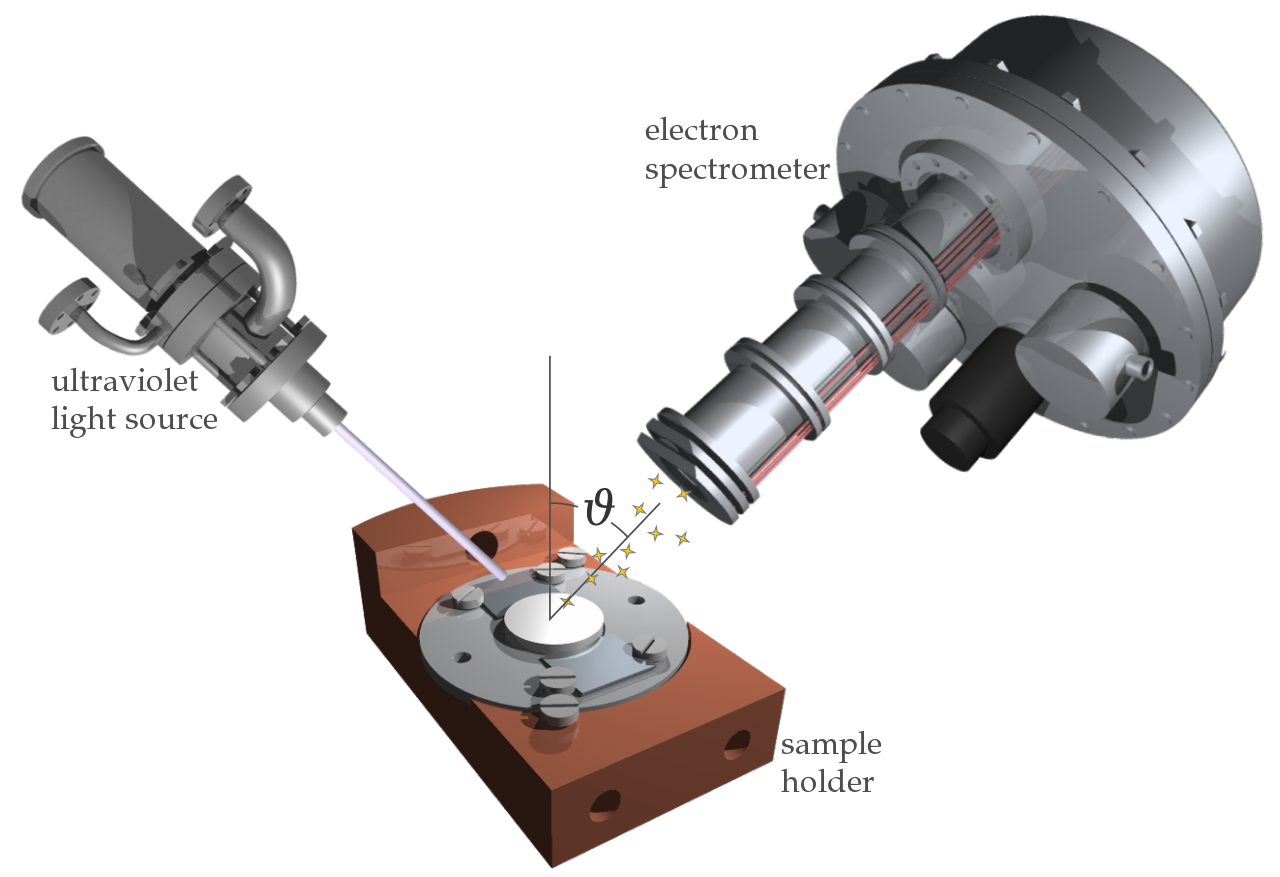
\includegraphics[width=0.8\linewidth]{img/1280px-ARPES_setup_-_ultraviolet_source_-_sample_holder_-_electron_analyzer.svg.png}
    \caption{Typischer Aufbau eines ARPES Experiments: Eine Heliumlampe sendet ultraviolettes Licht auf eine Probe aus, die Elektronen werden vom Messkopf analysiert.
    \refimgsource{Wikimedia}{https://commons.wikimedia.org/wiki/File:ARPES_setup_-_ultraviolet_source_-_sample_holder_-_electron_analyzer.svg}{17.02.2022}{Creative Commons Attribution-Share Alike 4.0 International}}
    \label{fig:arpes}
\end{figure}

\begin{figure}[!ht]
    \centering
    \begin{subfigure}[t]{0.45\textwidth}
        \centering
        \begin{tikzpicture}
            \begin{axis}[
                xmin=-1.3, xmax=1.3,
                ymin=0., ymax=1.5, 
                xlabel={$k_{\mathrm{mat},\parallel}$}, ylabel={$k_{\mathrm{mat},\bot}$}, 
                xtick = {-1, 1},
                xticklabels= {$-\sqrt{2 m E_{\mathrm{vac}}}$, $\sqrt{2 m E_{\mathrm{vac}}}$},
                ytick = {0, 1, 1.4142},
                yticklabels = {$0$, $k_\bot^{(1)}$,  $k_\bot^{(2)}$},
                grid=both,
                width=.9\textwidth]
                \addplot[domain = -3.14:3.14,smooth,samples=500, thick] ({cos(deg(x))}, {sqrt(sin(deg(x))^2 + 1)});
            \end{axis}
        \end{tikzpicture}
        \subcaption{Skizze des ARPES Ergebnisses mit Materialkonstanten $V_O$ und $k_\bot^{(1)} = \sqrt{2 m V_O}$ sowie  $k_\bot^{(2)} = \sqrt{2 m (V_O + E_{\mathrm{vac}})}$.}
    \end{subfigure}
    \begin{subfigure}[t]{0.45\textwidth}
        \centering
        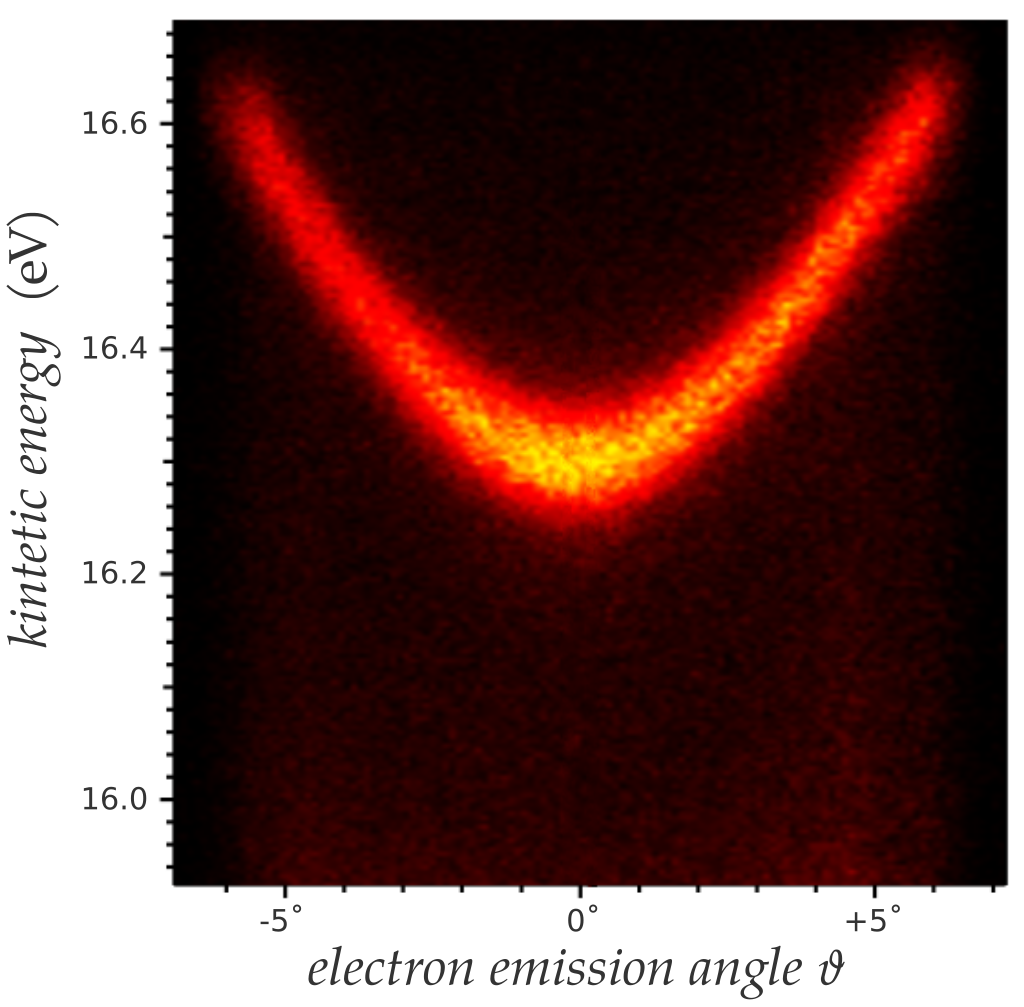
\includegraphics[width=.8\linewidth]{img/ARPES_-_Cu(111)_surface_state_-_21.22eV_300K.svg.png}
        \subcaption{Angle-resolved photoemission (ARPES) spectrum of a Cu(111) surface state using $\SI{21.22}{eV}$ photons at $T=\SI{300}{K}$. Intensity is color coded as electron counts per kinetic energy and emission angle channel. Fermi level is imaged at $\SI{16.64}{eV}$. }
    \end{subfigure}
    \caption{Ergebnis einer ARPES-Messung. \refimgsource{Wikimedia}{https://commons.wikimedia.org/wiki/File:ARPES_-_Cu(111)_surface_state_-_21.22eV_300K.svg}{17.02.2022}{ Creative Commons Attribution-Share Alike 4.0 International}}
    \label{fig:arpes result}
\end{figure}

\begin{fquestion}{Wie bestimmt man beim ARPES die elektrische Struktur?}
    Der Versuchsaufbau ist in \autoref{fig:arpes} schematisch dargestellt.
    Es werden Photonen der Energie $E_{\mathrm{Ph}} = h \nu$ auf die Probe geschickt. 
    Dort verrichtet das Photon Auslösearbeit $E_B$ und löst durch inelastische Vibrationsanregung ein Elektron.
    Dieses Elektron hat am Ende die Energie $E_{\mathrm{mat}} = E_{\mathrm{Ph}} - E_B$. 
    Zusätzlich hat das Elektron einen Impuls $\Vec{k}_{\mathrm{mat}}$.
    
    Damit es das Material verlassen kann muss zusätzlich Oberflächenarbeit $V_O$ geleistet werden, im Vakuum hat das Elektron also die Energie $E_{\mathrm{vak}} = E_{\mathrm{mat}} - V_O$; bei diesem Prozess ändert sich lediglich die Impulskomponente senkrecht zur Oberfläche.
    
    Mithilfe der Dispersionsrelation $E = \frac{\hbar^2}{2m} |k|^2$ und $\cos \theta = {|k_{\mathrm{vac},\parallel}|}/{|k_{\mathrm{vac}}|} = {|k_{\mathrm{mat},\parallel}|}/{|k_{\mathrm{mat}}|}$ kann man schließlich den Elektronenimpuls im Material charakterisieren:
    $$\begin{aligned} 
    |k_{\mathrm{mat}, \parallel}| &= \sqrt{\frac{2 m E_{\mathrm{vac}}}{\hbar^2}} \cos \theta, \\
    |k_{\mathrm{mat}, \bot}| &= \sqrt{\frac{2 m}{\hbar^2} (E_{\mathrm{vac}} \sin^2 \theta  + V_O)}.
    \end{aligned}$$
    % {\begin{align*}
    %     |k_{\mathrm{mat}, \parallel}| &= \sqrt{\frac{2 m E_{\mathrm{vac}}}{\hbar^2}} \cos \theta & |k_{\mathrm{mat}, \bot}| &= \sqrt{\frac{2 m}{\hbar^2} (E_{\mathrm{vac}} \sin^2 \theta  + V_O)} &
    % \end{align*}}
    In der Realität ist $V_O = E_F$, damit lässt sich die Fermioberfläche durch ARPES vermessen.
    Der Zusammenhang ist in \autoref{fig:arpes result} dargestellt.
\end{fquestion}

% \begin{question}{Was für eine Anregung ist das?}
%      Es ist eine inelastische Vibrationsanregung.
% \end{question}

\begin{fquestion}{Warum nutzt man keine Photonen?}
     Die Dispersionsrelation von Photonen ist linear mit sehr steilem Anstieg, man kann also nur nahe $k=0$ messen.
     Mit Röntgen-Licht benötigt man eine sehr hohe Präzision bei der Energiemessung, um die Phononen auflösen zu können, da $E_\gamma \sim 1\,$keV und $E_\mathrm{phonon} \sim 10\,$meV.
     Inzwischen können solche Experimente aber tatsächlich durchgeführt werden \cite{Bur2000}.
    %  alternativ Röntgen-Licht, aber trotzdem schwierig, weil Energieunterschied sehr gering (noch andere Effekte problematisch) ??? 
\end{fquestion}

\begin{fquestion}{Warum nicht mit Elektronen?}
    Die freie Weglänge von Elektronen in Festkörpern ist sehr gering, daher dringen sie nicht tief genug ein. 
\end{fquestion}

\begin{fquestion}{Warum nennt man einen Zweig akustisch?}
    Akustische Phononen (auch als Schallquanten bezeichnet) sind die Quanten der Schallwellen, die sich durch das Kristallgitter fortpflanzen. 
    Im Zentrum der Brillouin-Zone bewegen sich benachbarte Atome gleichsinnig.
\end{fquestion}

\begin{fquestion}{Warum nennt man einen Zweig optisch?}
    Bei optischen Phononen bewegen sich die Atome innerhalb der Basis gegeneinander. 
    
    Die Bezeichnung „optisch“ beruht darauf, dass in Ionenkristallen wie NaCl benachbarte Ionen meist entgegengesetzte Ladung tragen und dadurch auch durch elektromagnetische Wellen angeregt werden können. 
    Die mechanischen Schwingungen entsprechen dann elektrischen Dipolschwingungen, die je nach Schwingungsfrequenz der Phononen oft im Bereich des infraroten oder sichtbaren Lichts liegen.
\end{fquestion}

\begin{figure}[ht!]
    \centering\def\phase{187}
    \begin{subfigure}[t]{0.48\linewidth}
        \begin{tikzpicture}[]
            \begin{axis}[
                  axis x line=none,
                  axis y line=none,
                  domain=-195:195,
                  samples=201,
                  xticklabels=\empty,
                  width=1.25\linewidth,
                  height=0.75\linewidth
                ]
               \addplot [black, thick] {sin(x + \phase)};
               \node[shape=circle,fill=blue!25,draw,inner sep=2pt] at (axis cs:-180,{sin(-180 + \phase)}) {+};
               \node[shape=circle,fill=green!25,draw,inner sep=2pt] at (axis cs:-135,{sin(-135 + \phase)}) {-};
               \node[shape=circle,fill=blue!25,draw,inner sep=2pt] at (axis cs:-90,{sin(-90 + \phase)}) {+};
               \node[shape=circle,fill=green!25,draw,inner sep=2pt] at (axis cs:-45,{sin(-45 + \phase)}) {-};
               \node[shape=circle,fill=blue!25,draw,inner sep=2pt] at (axis cs:0,{sin(0 + \phase)}) {+};
               \node[shape=circle,fill=green!25,draw,inner sep=2pt] at (axis cs:45,{sin(45 + \phase)}) {-};
               \node[shape=circle,fill=blue!25,draw,inner sep=2pt] at (axis cs:90,{sin(90 + \phase)}) {+};
               \node[shape=circle,fill=green!25,draw,inner sep=2pt] at (axis cs:135,{sin(135 + \phase)}) {-};
               \node[shape=circle,fill=blue!25,draw,inner sep=2pt] at (axis cs:180,{sin(180 + \phase)}) {+};
        	\end{axis}
        \end{tikzpicture}
        \subcaption{Akustische Mode}
    \end{subfigure}
    \begin{subfigure}[t]{0.48\linewidth}
        \begin{tikzpicture}[]
            \begin{axis}[
                  axis x line=none,
                  axis y line=none,
                  domain=-195:195,
                  samples=201,
                  xticklabels=\empty,
                  width=1.25\linewidth,
                  height=0.75\linewidth
                ]
               \addplot [blue!25!black, thick] {sin(x + \phase)};
               \addplot [green!25!black, thick] {sin(x + \phase + 180)};
               \node[shape=circle,fill=blue!25,draw,inner sep=2pt] at (axis cs:-180,{sin(-180 + \phase)}) {+};
               \node[shape=circle,fill=green!25,draw,inner sep=2pt] at (axis cs:-135,{sin(-135 + \phase + 180)}) {-};
               \node[shape=circle,fill=blue!25,draw,inner sep=2pt] at (axis cs:-90,{sin(-90 + \phase)}) {+};
               \node[shape=circle,fill=green!25,draw,inner sep=2pt] at (axis cs:-45,{sin(-45 + \phase + 180)}) {-};
               \node[shape=circle,fill=blue!25,draw,inner sep=2pt] at (axis cs:0,{sin(0 + \phase)}) {+};
               \node[shape=circle,fill=green!25,draw,inner sep=2pt] at (axis cs:45,{sin(45 + \phase + 180)}) {-};
               \node[shape=circle,fill=blue!25,draw,inner sep=2pt] at (axis cs:90,{sin(90 + \phase)}) {+};
               \node[shape=circle,fill=green!25,draw,inner sep=2pt] at (axis cs:135,{sin(135 + \phase + 180)}) {-};
               \node[shape=circle,fill=blue!25,draw,inner sep=2pt] at (axis cs:180,{sin(180 + \phase)}) {+};
        	\end{axis}
        \end{tikzpicture}
        \subcaption{Optische Mode}
    \end{subfigure}
    \caption{Phononenmoden der zweiatomigen Basis}
    \label{fig:phononenmoden}
\end{figure}


\begin{fquestion}{Wie äußern sich die Moden bei einer zweiatomigen Basis?}
    Ein Vergleich von optischen und akustischen Transversalwellen von Phononen bei 2-atomiger Basis für kleine $k$ ist in \autoref{fig:phononenmoden} dargestellt.
    \\
    Für $|k|\rightarrow \frac{\pi }{a}$ schwingt jeweils nur eine Atomsorte, wobei $\omega_+ = \sqrt{\frac{2C}{m}}$ und $\omega_- = \sqrt{\frac{2C}{M}}$ ist ($M > m$).
    Die Wellenlänge ist jeweils $\lambda = \frac{2\pi }{k} = 2a$.
\end{fquestion}

\begin{fquestion}{Was ist die Laue-Bedingung?}
    Die Impulsänderung $\Delta\Vec{k} = \Vec{k}_\mathrm{out} - \Vec{k}_\mathrm{in}$ muss einem reziproken Gittervektor $\Vec{G}$ entsprechen.
\end{fquestion}

\subsection{Magnonen}

\begin{figure}[ht!]
    \centering
    \animategraphics[autoplay, width=0.5\textwidth,loop]{15}{img/spin_wave/Spin_wave-}{1}{2}
    \caption{Animation einer Anregung in der Mitte eines Spin-Feldes. Die Anregung propagiert durch den Drehmomente und damit den Austausch von Drehimpuls.
    \refimgsource{Wikimedia}{https://commons.wikimedia.org/wiki/File:Spin_wave.gif}{18.01.2022}{public domain}}
\end{figure}

\begin{fquestion}{Was sind Magnonen?}
    Magnonen sind bosonische Quasiteilchen; sie treten bspw. in Festkörpern als quantisierte Spinwellen auf (analog zum Phonon als quantisierte Schallwelle).
\end{fquestion}

\begin{fquestion}{Wie ist die Dispersionsrelation der Magnonen?}
    Für Magnonen im Ferromagneten gilt die Dispersionsrelation 
    \[ \hbar \omega = 4 J S (1 - \cos a k) \approx 2 J S a^2 k^2 := D k^2 \]
    mit $D = 2 J S a^2 \approx \SI{281}{\milli\electronvolt\angstrom\squared}$, wobei $J$ die Kopplungskonstante, $S$ der Betrag des Spins und $a$ die Gitterkonstante sind.
\end{fquestion}


% \begin{question}{Warum ist die Kurve der Dispersionsrelation am Rand der Brillouin Zone abgeflacht? }
%     Welle wird am Rand der BZ reflektiert und es bildet sich eine stehende Welle, Gruppengeschwindigkeit 0 und daher die Ableitung der Dispersionrelation auch Null
% \end{question}

% \begin{question}{Was sind die masselosen und massiven Anregungen des Systems?}
%     Im Potential gezeigt, dass masselos (Nambu-Goldstone-Anregung) entlang Kreis im Hut-Potential (also 3D-Doppelmuldenpotential) ohne Änderung der potentiellen Energie und massiv (Higgs-Anregung) "entlang Potentialwände"
% \end{question}


% \begin{question}{Was stellen die Anregungen allgemein dar?}
%     einmal Fluktuation ohne betraglicher Änderung des OP, einmal mit
% \end{question}

\begin{fquestion}{Was ist der Unterschied zwischen massiven und masselosen Spinwellen?}
    Die massiven Magnonen sind lokale Störungen der Magnetisierung, die sich wellenartig ausbreiten können ($\si{\micro\electronvolt}$).
    Die masselosen Anregungen ($\lambda = \infty$) beschreiben Spindrehung des gesamten Ferromagneten ohne betraglicher Änderung der Magnetisierung.
\end{fquestion}

\begin{fquestion}{Was passiert mit einzelnen Spins bzw. den Anregungen nahe der kritischen Temperatur?}
    Knapp unterhalb der kritischen Temperatur ist die Wahrscheinlichkeit sich parallel zu den benachbarten Momenten auszurichten etwas größer als die einer willkürlichen Ausrichtung. 
    Oberhalb der kritischen Temperatur ist es entsprechend andersherum.
\end{fquestion}

% \begin{question}{Wie kann man die Anregungen vermessen?}
%     Inelastische Neutronenstreuung, kurz bisschen was dazu erzählt ???
% \end{question}

% \begin{question}{Wie kann man denn so ein Magnon unendlicher Wellenlänge verstehen? }
%     Spindrehung des gesamten Ferromagneten, d.h. alle Spins drehen sich kollektiv in eine Richtung 
    
%     Betrag der Magnetisierung ändert sich nicht, nur die Richtung
% \end{question}

\begin{fquestion}{Wie kann man Magnonen messen?}
    Durch Neutronenstreuung: Das magnetische Moment des Neutron ($\mu_n = \frac{e \hbar}{2 m_p}$, entsteht durch die Konstituentenquarks) wechselwirkt mit den magnetischen Momenten der Elektronen und entsprechend kann man deren Verteilung messen.
    In Kernreaktoren oder dur Spallationsquellen (Beschuss von Atomkernen mit schnellen $> \SI{100}{\mega\electronvolt}$ Projektilen) können schnelle Neutronen freigesetzt werden.
    Da das magnetische Moment des Neutron viel kleiner als dessen Masse ist, müssen die Neutronen vorher abgebremst werden, damit die Wechselwirkung mit den Magnonen überhaupt beobachtet werden kann.
    
    Auf anderem Weg können Magnonen über Experimente mit dünnen Ferromagneten und hochfrequenten Magnetfeldern bestimmt werden.
\end{fquestion}

% \begin{question}{Wo kommt das magnetische Moment des Neutrons her? }
%     Unterstruktur der Valenzquarks führt zu $\mu = g_n \mu_{\mathrm{Kern}} S$
% \end{question}

% \begin{question}{Was sind Quellen von Neutronen? }
%     Reaktor oder Spallationsquelle, müssen aber üblicherweise noch abgebremst werden ???    
% \end{question}

\subsection{Festkörper}

\begin{fquestion}{Wie kommt der elektrische Widerstand im Festkörper zustande?}
    Die elektrische Leitfähigkeit ist durch
    $$\sigma = \frac{n e^2 \lambda_F}{m^\star v_F}$$
    gegeben, wobei $n$ die Elektronendichte, $\lambda_F$ die mittlere freie Weglänge für Elektronen mit Fermi-Energie, $m^\star$ die reduzierte Masse und $v_F$ die Fermi-Geschwindigkeit sind.
    
    Phänomenologisch entsteht der elektrische Widerstand durch die Streuung von Elektronen an den Phononen des Kristallgitter (deren An- bzw. Abregung) und an Störstellen im Kristall bei ihrer thermischen Geschwindigkeit.
    Eine Streuung an anderen Elektronen oder Atomrümpfen findet selten statt.
\end{fquestion}


\begin{fquestion}{Wie sieht die Dispersionsrelation für Elektronen aus?}
    Die Dispersionsrelation für Elektronen ist quadratisch $E \propto k^2$, durch das Entstehen von stehenden Wellen am Rand der Brillouin-Zone flacht diese dort ab. 
    Die entsprechende Bandstruktur kann durch das Umklappen der Dispersionsrelationen am Rand der Brillouin-Zone erhalten werden:
    \begin{center}
        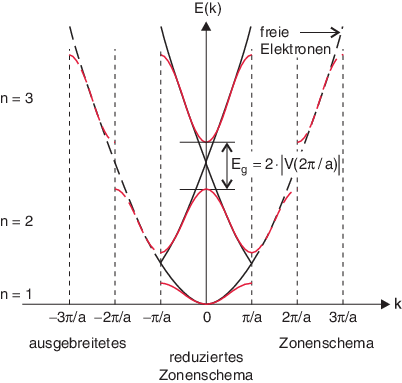
\includegraphics[width=0.7\linewidth]{img/32672_5_De_13_Fig13_HTML.png}
    \end{center}
    
    \refimgsource{Elektronen im Festkörper}{https://media.springernature.com/lw785/springer-static/image/chp\%3A10.1007\%2F978-3-662-49094-5_13/MediaObjects/32672_5_De_13_Fig13_HTML.gif}{14.02.2022}{Keine}
\end{fquestion}
    
\begin{fquestion}{Was passiert, wenn sich zwei Elektronenbänder kreuzen?} 
    Beim Kreuzen zweier Energiebänder wären die Zustände eigentlich entartet, physikalisch entspricht diese Situation zwei stehenden Wellen mit gleicher Wellenlänge und Frequenz.
    Im Festkörper findet allerdings eine zusätzliche Auszeichnung durch die Phase beider Wellen statt.
    Entweder ist die Phase so, dass die Aufenthaltswahrscheinlichkeit ihr Minima genau bei oder entsprechend genau zwischen den Atomrümpfen hat, wodurch sich im ersten Fall eine stärkere Bindung als im zweiten Fall einstellt.
    Entsprechend entsteht eine Bandlücke.
    
    (Argumentation der vermiedenen Kreuzung eventuell auch über den effektiven Massetensor)
\end{fquestion}

\begin{fquestion}{Wie bestimmt man die Zustandsdichte?}
    Allgemein definiert man die Zustandsdichte über
    $$D(E) := \int_{\mathbb{R}^d} \delta(E - E_{\Vec{k}})\,\frac{\mathrm{d}^dk}{(2\pi)^d}, $$
    wobei $d$ die Dimension ist.
    Mit $E=\frac{k^2}{2m}$ und bei Vernachlässigung von Spins ergibt sich daraus dann 
    $$D(E) = \frac{1}{(2\pi)^d }\int_0^\infty \delta \left( E - \frac{k^2}{2m} \right)\, \underbrace{\frac{d\pi^{d/2}k^{d-1}}{\Gamma \left(\frac{d}{2} + 1\right) }}_{\text{Kugeloberfläche}} \,\mathrm{d}k.$$
    Da $\delta \left( E - \frac{k^2}{2m} \right) \equiv \frac{\delta (k-\sqrt{2mE})}{|k/m|}$ ist, folgt letztlich
    $$D(E) = \frac{d\pi^{d/2}(2mE)^{\frac{d-1}{2}}}{(2\pi)^d \Gamma \left(\frac{d}{2} + 1\right)} \frac{m}{\sqrt{2mE}} \propto (2mE)^{\frac{d}{2} - 1} \equiv k^{d-2}.$$
    % Die Zustandsdichte ist definiert als $D(E) := \frac{\mathrm{d}N}{\mathrm{d}E}$, woraus
    % $$N = \int_0^{E_F} D(E) \,\mathrm{d}E = \int_{\mathbb{R}^3} Z(\Vec{k}) \mathrm{d}^3k$$
    % mit der mikrokanonischen Zustandssumme $Z(\Vec{k})$ im Impulsraum durch $$Z(\Vec{k}) = \underbrace{2\cdot}_{\mathrm{Spins}} \frac{V}{(2\pi)^3}$$
    % gegeben.
    % Daraus folgt dann über $E=\frac{k^2}{2m}$ auch 
    % $$\mathrm{d}N = D(E)\, \mathrm{d}E = \frac{2V}{(2\pi)^3} 4\pi k^2\,\mathrm{d}k = \frac{8\pi Vk^2}{(2\pi)^3} \frac{1}{2} \sqrt{\frac{2m}{E}} \,\mathrm{d}E,$$
    % also $D(E) = \frac{mV}{\pi^2}\sqrt{2mE}$.
    
\end{fquestion}

\begin{fquestion}{Wie hängen Fermi-Impuls $k_F$ und die Spin-$\frac{1}{2}$-Fermionendichte zusammen?}
    Es ist $n=\frac{N}{V} = \frac{1}{V} \cdot \frac{V}{(2\pi)^3}\cdot \frac{4\pi}{3}k_F^3 = \frac{k_F^3}{6\pi^2}$ die Besetzungszahldichte.
    Da jeder Zustand von zwei Fermionen besetzt werden kann, ist $n_{1/2} = 2n$.
    Also gilt $k_F = \sqrt[3]{3\pi^2 n_{1/2}}$.
\end{fquestion}

\begin{fquestion}{Wie könnte man diesen Ausdruck für einen symmetrischen Kern noch vereinfachen?}
    Symmetrisch bedeutet hier $N=Z=\frac{A}{2}$.
    Mit $V\simeq \frac{4\pi}{3} R^3$ und $R\simeq R_0 A^{1/3}$ folgt dann 
    $$k_F \simeq \sqrt[3]{3\pi^2 \frac{A}{\frac{4\pi}{3}R_0^3 A}} = \frac{3}{2R_0}\sqrt[3]{\frac{2\pi}{3} }.$$
    Insbesondere gilt für den Fermi-Impuls der Protonen bzw. Neutronen dann $k_F^{\text{p}/\text{n}} = \frac{3}{2R_0}\sqrt[3]{\frac{\pi}{3} }$, weil nur die halbe Nukleonenzahl $\frac{A}{2}$ in die ``Gesamtanzahl'' an Fermionen eingeht.
\end{fquestion}

\begin{fquestion}{Wie könnte man damit grob die Fermi-Energie von Kernen abschätzen?}
    Die Fermi-Energie ist etwa $E_F=\frac{k_F^2}{2m} \simeq \frac{9}{8mR_0^2} \left(\frac{\pi}{3}\right)^{2/3}$.
    Für einen (symmetrischen) Kern gilt mit $R_0 \approx \SI{1.2}{fm}$ also 
    $$E_F \approx \frac{9\cdot (\SI{200}{MeV\femto\metre})^2}{8\cdot \SI{1000}{MeV} \cdot (\SI{1.2}{fm})^2 } \cdot 1.03 \approx \SI{32}{MeV}. $$
\end{fquestion}

\begin{fquestion}{Wie würde man die Fermi-Energie von einem Gold-Atom und einem weißen Zwerg abschätzen?}
    Allgemein gilt $E = \frac{k_F^2}{2m} = \frac{1}{2m} \left( 3\pi^2 n_{1/2} \right)^{2/3}$, man muss also die Masse und die Fermionendichte abschätzen.
    \\
    Gold liegt üblicherweise in einem fcc-Gitter vor, es gibt also $8\cdot \frac{1}{8} + 6\cdot\frac{1}{2} = 4$ Atome pro Zelle.
    Unter der Annahme, dass jeweils ein Elektron pro Atom frei ist, und dass die Kantenlänge $a$ der Zelle etwa $2\sqrt{2} r_0$ ist (Atome berühren sich auf der Diagonalen), folgt dann $k_F = \sqrt[3]{3\pi^2 \frac{4}{a^3}} \approx \SI{2}{keV}$ (Radius von Gold ist $r_0\approx \SI{166}{pm}$).
    Die Fermi-Energie ist somit $E_F \approx \frac{(\SI{2}{keV})^2}{2\cdot \SI{0.5}{MeV}} = \SI{4}{eV}.$
    \\
    Im Stern können wir annehmen, dass (fast) alle Elektronen frei sind, also ist 
    $$N_{1/2} \approx 26\cdot \frac{m_\mathrm{Stern}}{m_\mathrm{Fe}} \approx 26\cdot \frac{\SI{2e30}{kg}}{56m_n} \approx \SI{3e56}.$$
    Das Volumen ist $V = \frac{4\pi }{3} R_\mathrm{Stern}^3 \approx \SI{1.4e21}{m^3}$ ($R_\mathrm{Stern} \approx \SI{7e6}{m}$, also etwa 1\,\% des Sonnenradius).
    Der Fermi-Impuls ist damit $k_F \approx \sqrt[3]{3\pi^2 \frac{N_{1/2} }{V}} \approx \SI{1.8e12}{m^{-1}}$.
    Die Fermi-Energie folgt dann zu $E_F \approx \SI{0.13}{MeV}$.
    Das ist von dem tatsächlichen Wert von $0.3\,$MeV allerdings deutlich entfernt, die Abschätzung ist dafür viel zu ungenau.
\end{fquestion}

\begin{fquestion}{Warum tragen die Eisen-Kerne nicht zur Fermi-Energie bei?}
    Die Eisen-Kerne sind Bosonen, da ${}^{56}_{26}\mathrm{Fe}$ gerade Proton- und Neutronzahl hat, der Spin ist also ganzzahlig.
\end{fquestion}

\begin{fquestion}{Welches Kopplungsschema ist wann relevant?}
    LS: Die Coulomb-Abstoßung der Elektronen ist groß gegenüber der Spin-Bahn-Wechselwirkung, also gilt näherungsweise $$\begin{aligned}\Vec{L} &= \sum \Vec{l}_k, && \mathrm{und} & \Vec{S} &= \sum \Vec{s}_k\end{aligned}.$$
    Der Gesamtdrehimpuls ist dann $\Vec{J} = \Vec{L} + \Vec{S}$.
    Das gilt meist für leichte Kerne ($Z\lesssim 30$).
    \\
    jj: Die Spin-Bahn-Wechselwirkung groß gegenüber der Coulomb-Abstoßung, also können sich $\Vec{l}_k$ und $\Vec{s}_k$ nicht mehr unabhängig voneinander ausrichten.
    Phänomenologisch kann man argumentieren, dass durch $\Delta E_{LS} \sim \langle \Vec{l}\cdot\Vec{s} \rangle$ der ``Winkel'' zwischen den Vektoren ``fest'' ist.
    Dann koppeln die einzelnen Drehimpulse zu $\Vec{j}_k = \Vec{l}_k + \Vec{s}_k$, und es gilt dann
    $$\Vec{J} = \sum \Vec{j}_k.$$
    Das tritt vor allem für schwere Kerne auf ($Z\gtrsim 30$).
    
    Beides sind aber nur Näherungen. 
    Insbesondere tritt jj-Kopplung beispielsweise auch bei starken externen Magnetfeldern auf (siehe Paschen-Back-Effekt).
\end{fquestion}

\begin{fquestion}{Wie kann die Spin-Bahn-WW noch überwunden werden?}
    Mit einem externen Magnetfeld, siehe auch Zeeman- bzw. Paschen-Back-Effekt.
\end{fquestion}

\begin{fquestion}{Was besagen die Hund'schen Regeln?}
    Es ist derjenige elektronische Zustand mit maximalem Gesamtspin $S$ bevorzugt.
    Falls mehrere Zustände möglich sind, soll auch der Bahndrehimpuls $L$ maximal sein.
    Die Regeln beruhen auf der Coulomb-Abstoßung und maximieren (näherungsweise) den mittleren Abstand zwischen den Elektronen, und minimieren damit die Energie.
\end{fquestion}

\begin{fquestion}{Wie werden d-Orbitale von 6 Elektronen besetzt?}
    Es gibt $2(2l + 1) = 10$ Orbitale ($2l+1$ verschiedene $m_L$ und je zwei $m_S$), von denen 6 besetzt werden sollen.
    Nach den Hund'schen Regeln verteilen wir die ersten 5 Elektronen so, dass alle parallelen Spin haben. 
    Das letzte Elektron hat dann entsprechend umgekehrten Spin, und besetzt das $m_L=2$-Orbital, also $S=2$.
    Damit ist der Spin $S= \frac{1}{2}(5 - 1) = 2$ und der Bahndrehimpuls $L=2$, also $J = 0\dots 4$.
\end{fquestion}

\begin{fquestion}{Warum ist es kein Widerspruch, dass die Elektronen bei LCAO bevorzugt zwischen den Kernen sind und im Festkörper bevorzugt an den Kernen?}
    Beide Phänomene haben ihren Ursprung in der LCAO- bzw. Tight-Binding-Methode.

    Bei der LCAO-Methode wird die Orbitalstruktur von Molekülen untersucht; dabei gilt die Annahme dass sich die gemeinsame Molekülorbitalstruktur aus den Atomorbital zusammensetzt. 
    Beim Wasserstoff entsteht hierbei ein symmetrischer und ein anti-symmetrischer Grundzustand, wobei nur der symmetrische Zustand zu einer energetisch günstigen Bindung führt.
    Die beiden Elektronen des Wasserstoff sind also symmetrisch gebunden, wobei der symmetrische Zustand eine nicht verschwindende Aufenthaltswahrscheinlichkeit zwischen den Kernen hat.
    
    Beim Festkörper betrachten wir quasi-freie Elektronen, die schwach mit dem Kristallgitter wechselwirken. 
    Für ein einzelnes Elektron wird wieder das Atomorbital lokalisiert einem Gitterplatz als Wellenfunktion beibehalten.
    Durch die anderen Gitterplätze kommt es zu mehreren wichtigen Matrixelementen:
    \begin{itemize}
        \item Der (meist kleinen) Absenkung der Eigenenergie durch das Potential der anderen Gitterplätze,
        \item dem Bindungsterm (der den Potentialerwartungswert des Überlapps zweier Elektronen an verschiedenen Gitterplätzen beschreibt) und
        \item dem Überlappterm.
    \end{itemize}
    Durch die Form des Gitters ist es nun energetisch günstig sich bei einem Atomrumpf zu positionieren. 
    Nach dem Bloch-Theorem muss sich die Wellenfunktion um die Gitterkonstante verschieben lassen, bei einem stark-bindenden Festkörper würden zwischen den Rümpfen lokalisierte Elektronen also weniger stark gebunden sein als bei den Rümpfen gebundene.
    Die Potentialreichweite der Rümpfe ist klein, ergo ist der Verlust beim Überlapp mit dem eigenen Atomrumpf so gravierend dass er nicht durch den zusätzlichen Überlapp mit dem benachbarten Atomrumpf kompensiert werden kann.

    % bei LCAO für Bindung verantwortlich, im FK sind sie quasifrei ??? 
    Dass beim Wasserstoff die Bindung mit Lokalisierung des Elektrons zwischen den beiden Kernen und beim Festkörper die Lokalisierung des Elektrons bei den Atomrümpfen energetisch günstiger sind folgt anschaulich also jeweils aus der Symmetrie des Problems. 
\end{fquestion}


\cleardoublepage
\section{Energieniveaus und Übergänge}
\addcontentsline{qst}{section}{\thesection \hspace{.5em} Energieniveaus und Übergänge}
\subsection{Primäre Energieskalen}

\begin{fquestion}{Energieeigenwerte im Wasserstoffatom?}
    $E_n = \frac{E_R}{n^2}$ mit Rydberg-Energie $E_R = \alpha^2  \frac{\mu}{2} = 13.6\,$eV.
\end{fquestion}

\begin{fquestion}{Wie ist die Feinstrukturkonstante definiert? }
    $\alpha = \frac{e^2}{4\pi\epsilon_0\hbar c} \approx \frac{1}{137}$
\end{fquestion}

\begin{fquestion}{Ohne Feinstruktur, was gibt es noch für Niveaus?}
    Ohne Feinstruktur ist die Energie noch unabhängig von der Drehimpulsquantenzahl $l$.
    Selbst mit Feinstruktur ist die Energie aber unabhängig von der $z$-Komponente, also der Quantenzahl $m = -l, \dots , l$.
    Das muss auch so sein, weil $m$ lediglich die Projektion von $\Vec{L}$ auf eine willkürlich gewählt Achse (hier die $z$-Achse) beschreibt.
    Die Skizze dieser Projektion 
    \begin{center}
        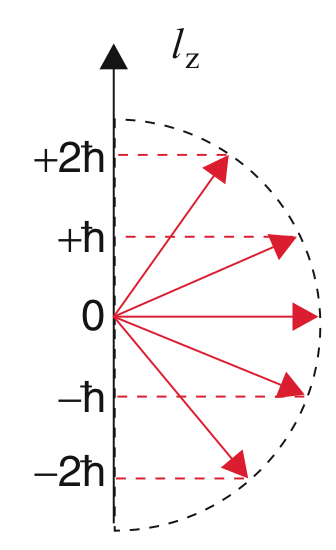
\includegraphics[width=0.25\linewidth]{img/Projektion_Magnetquantenzahl.png}
    \end{center}
    Abbildung unverändert aus ``Demtröder: Experimentalphysik 3 -- Atome, Moleküle und Festkörper, S. 151''. 
    \\
    Das ist auch für beliebige andere Zentralpotentiale der Fall.
    Mathematisch kann man auch über den Separationsansatz argumentieren, da $m$ nicht in der Radialgleichung auftaucht, und damit die Energie nicht beeinflussen kann.
\end{fquestion}

\begin{fquestion}{Wie kann man grob Grundzustand und Bindungsradius abschätzen?}
    Heisenberg-Unschärfe, z.B. $\Delta x \Delta p \simeq \hbar$.
    Daraus folgt $\Delta p \simeq \frac{1}{\Delta x}$ und $r_0 \simeq \frac{1}{p_0}$.
    Dabei ist $E_\text{kin} = \frac{p_0^2}{2\mu} \simeq \frac{1}{2\mu r_0^2}$.
    Für das Coulomb-Potential ist
    $$E = E_\text{kin} + E_\text{pot} = \frac{1}{2\mu r^2} - \frac{\alpha}{r},$$
    wobei das Minimum durch $0 = -\frac{1}{\mu r_0^3} + \frac{\alpha}{r_0^2}$, also $r_0 = \frac{1}{\mu\alpha} $, gegeben ist.
    Die Grundzustandsenergie ist damit etwa $E_0 \simeq \frac{1}{2\mu r_0^2} = \alpha^2\frac{\mu }{2}$.
\end{fquestion}

\begin{fquestion}{Was sind die Quantenzahlen bei Wasserstoff?}
    Hauptquantenzahl $n$, (Bahn-)Drehimpulsquantenzahl $l$, magnetische Quantenzahl $m$ (oder auch $m_l$) und Spin $s$ (oder auch $m_s$).
\end{fquestion}

\begin{fquestion}{Wie sieht das beim Atomkern aus?}
    Analog, anstatt der (willkürlich eingeführten) Hauptquantzenzahl $n$ verwendet man hier die Knotenzahl $N$, wobei wieder $n = N+l+1$ gilt.
\end{fquestion}

\begin{fquestion}{Wie kommt das?}
    Das Experiment kam historisch vor der Theorie des Wasserstoff-Atoms, und die Energieniveaus konnten mit $n$ bequem abgezählt werden.
    Beim Atomkern war die Theorie dann bereits bekannt, weshalb hier $N$ verwendet wird.
    Anmerkung: Wäre die Theorie auch für Atome zuerst da gewesen, gäbe es $n$ möglicherweise gar nicht.
\end{fquestion}

\subsection{Sekundäre Energieskalen}

% \begin{fquestion}{Woher kommt die Zyklotronfrequenz?}
%     Ein Elektron in einem Zyklotron befindet sich klassisch betrachtet in einem Kräftegleichgewicht
%     $$|F_\text{L}| = |evB| \overset{!}{=} |m\omega v| = |F_p|. $$
%     Die Zyklotronfrequenz ist daher $\omega_B = \frac{eB}{m}$.
% \end{fquestion}

\begin{fquestion}{Was ist das Bohr-Magneton?}
    Es ist $\mu_B = \frac{e\hbar}{2m_e} = \SI{5.788e-4}{\frac{eV}{T}}$.
    
    Betrachte ein Elektron als eine klassische Ladung auf einer Kreisbahn.
    Dann ist das magnetische Moment über den Kreisstrom $I=\frac{e}{2\pi r}v$ und die Fläche $A=\pi r^2$ gegeben, also
    $$\mu_\mathrm{kl.} = IA = \frac{evr}{2} = \frac{e\hbar}{2m_e}\frac{m_e vr}{\hbar} \equiv \mu_B \frac{L}{\hbar}. $$
    Dabei ist $L = m_evr$ der klassische Bahndrehimpuls.
    Ersetzt man $L$ mit dem Spin $\frac{\hbar}{2}$, weicht das tatsächlich magnetische Moment um einen Faktor 2 von dem klassisch erwarteten Wert ab.
    Das ist gerade der $g_S$-Faktor, tatsächlich ist also
    $$\mu_S = g_S\mu_\mathrm{kl.} = g_S\frac{\mu_B}{2}$$
    mit $g_S\simeq 2$ (kleine Abweichungen durch QED).
    % Die ``naive'' (also klassische) Vorstellung eines Elektrons auf einer Kreisbahn liefert ebenfalls eine Herleitung 
\end{fquestion}

% \begin{question}{Wie kommt man auf das magnetische Moment des Elektrons?}
%     Elektron hat magnetisches Moment $\mu = g_S\mu_B S$ (wie kommt man auf $\mu_B$ ??? )
%     Magnetfeld proportional zum Drehimpuls ???
% \end{question}

\begin{fquestion}{Was ist die LS-Kopplung?}
    Die Energie eines magnetischen Dipols im Magnetfeld ist prinzipiell $\Delta E = -\Vec{\mu}\cdot\Vec{B}$.
    Im Ruhesystem des Elektrons gibt es ein effektives Magnetfeld des Nukleus.
    Allgemein gilt für elektromagnetische Zentralpotentiale $V(r) = (-e)\phi(r)$ der Zusammenhang
    $$\begin{aligned}
        \Vec{B} &= -\Vec{v} \times \Vec{E} = \frac{\Vec{p}}{m}\times\nabla \phi = \frac{\Vec{p} \times \Vec{e}_r}{m} \frac{V'(r)}{-e} = \frac{V'(r)}{m_eer}\Vec{L},
    \end{aligned}$$
    wobei $\Vec{L} = \Vec{r} \times\Vec{p}$ der Bahndrehimpuls ist.
    Mit dem Elektronenspin $\Vec{S}$ und $g_s \simeq 2$ gilt $\Vec{\mu} = -g_s \mu_B\Vec{S}$, wobei $\mu_B = \frac{e}{2m_e}$.
    Insgesamt ist die Energiekorrektur also gegeben durch
    $$\Delta E_{LS} = \frac{g_s\mu_B V'(r)}{m_eer}  \expval{\Vec{L} \cdot \Vec{S}}.$$
    Für das Coulomb-Potential folgt dann
    $$\Delta E_{LS} = \frac{\alpha g_s\mu_B}{m_ee}  \expval{\Vec{L} \cdot \Vec{S}} \expval{\frac{1}{r^3}},$$
    wobei 
    $$\expval{\frac{1}{r^3}} = \frac{1}{a_0^3n^3 l \left( l + \frac{1}{2} \right) (l+1)}.$$
    Mit $a_0 = \frac{1}{m_e\alpha}$ ist dann 
    $$\Delta E_{LS} = \alpha^4m_e g_s \frac{\expval{\Vec{L} \cdot \Vec{S}} }{2n^3 l \left( l + \frac{1}{2} \right) (l+1)}.$$
    Mit $\Vec{J} = \Vec{L} + \Vec{S}$, $S=\frac{1}{2}$ und $\Vec{\mu} = g_J \mu_B \Vec{J}$ kann man dann noch
    $$2\expval{\Vec{L} \cdot \Vec{S}} = \expval{\Vec{J}^2 - \Vec{L}^2 - \Vec{S}^2} = J(J+1) - L(L+1) - S(S+1)$$
    herleiten, was sich mit $|L-S|\le J\le L+S$, also $J = L \pm \frac{1}{2}$, zu 
    $$\expval{\Vec{L} \cdot \Vec{S}} = \begin{cases} \frac{l}{2}, & m_s = +\frac{1}{2} \\ -\frac{l+1}{2},& m_s = -\frac{1}{2} \end{cases}$$
    vereinfacht.
    % ??? Das stimmt doch irgendwie nicht ???
    % Kopplung Elektronenspin an Bahndrehimpuls
    % semiklasische Dipolformel $\langle\frac{\mu_1\mu_2}{r^3}\rangle$
    % Dirac-Formel $\frac{1}{r}\frac{\text{d}V}{\text{d}r}$ (betrachte $J=L+S$ und $\mu = g \mu_B J$)
\end{fquestion}

\begin{fquestion}{Gibt es die Formel auch in einfach?}
    Mit den Näherungen $g_S\approx 2$ und $|\langle \Vec{L}\cdot\Vec{S} \rangle| \approx \frac{l}{2}$ kann man die Energiekorrektur näherungsweise über
    $$\Delta E_{LS} \simeq -E_n\frac{\alpha^2}{nl(l+1)}. $$
    beschreiben.
    Die maximale Aufspaltung ergibt sich für 2p, also $n=2$ und $l=1$.
    % beschreiben, wobei $|\expval{\Vec{L}\cdot\Vec{S}}| \approx \frac{l}{2}$ und $g_S\approx 2$ angenommen werden.
\end{fquestion}

\begin{fquestion}{Wie kommt man damit auf die $\alpha^4$-Abhängigkeit?}
    Siehe die Herleitung der obigen Frage. 
    Für die $\alpha^4$-Abhängigkeit war aber entscheidend, dass $\langle \frac{1}{r^3} \rangle \sim \alpha^3$ gilt.
    Da man aber natürlich $\langle \frac{1}{r^3} \rangle \sim \frac{1}{a_0^3}$ erwarten kann, folgt dieser Zusammenhang direkt.
    Die $\frac{1}{r^3}$-Abhängigkeit muss man auch nicht präzise herleiten, sondern kann stattdessen mit der üblichen $\frac{1}{r^3}$-Abhängigkeit von Dipol-Wechselwirkungen argumentieren.
    % Abschätzung über V und r0, hängt mit Abstandsanhängigkeit der Dipol-WW zusammen
\end{fquestion}

\begin{fquestion}{Wie sieht verhält sich die Aufspaltung mit wachsender Kernladungszahl?}
    Es ist $\alpha \rightarrow Z\alpha$, also $\Delta E_{LS} \propto Z^4$.
    Allerdings muss man insbesondere für ``weiter außen gelgene'' Orbitale, also größere $l$, mit einer effektive Kernladung $Z_\mathrm{eff} < Z$ rechnen, da die Kernladung teilweise abgeschirmt wird.
\end{fquestion}

% \begin{question}{Wie hängen magnetisches Moment und Spin zusammen?}
%     gyromagnetisches Verhältnis
%     Definition des Bohr-Magnetons $\mu_B = \frac{e\hbar}{2m_e}$ aus Kreisstrom von Elektron um Proton ??? 
% \end{question}

\begin{fquestion}{Wie spaltet in der Feinstruktur das 2p-Niveau auf?}
    In $2\mathrm{p}_{1/2}$ und $2\mathrm{p}_{3/2}$, die Aufspaltung ist ohne Lamb-Shift und/oder Dirac sogar noch symmetrisch.  
    Insbesondere sind $2\mathrm{s}_{1/2}$ und $2\mathrm{p}_{1/2}$ hier noch entartet (auch mit Darwin-Term, siehe \autoref{fig:feinstruktur wasserstoff}).
    Die Entartung wird erst durch den Lamb-Shift aufgehoben, wobei $2\mathrm{s}_{1/2}$ dann energetisch höher liegt (etwa 1\,GHz). 
\end{fquestion}

\begin{figure}[!ht]
    \centering
    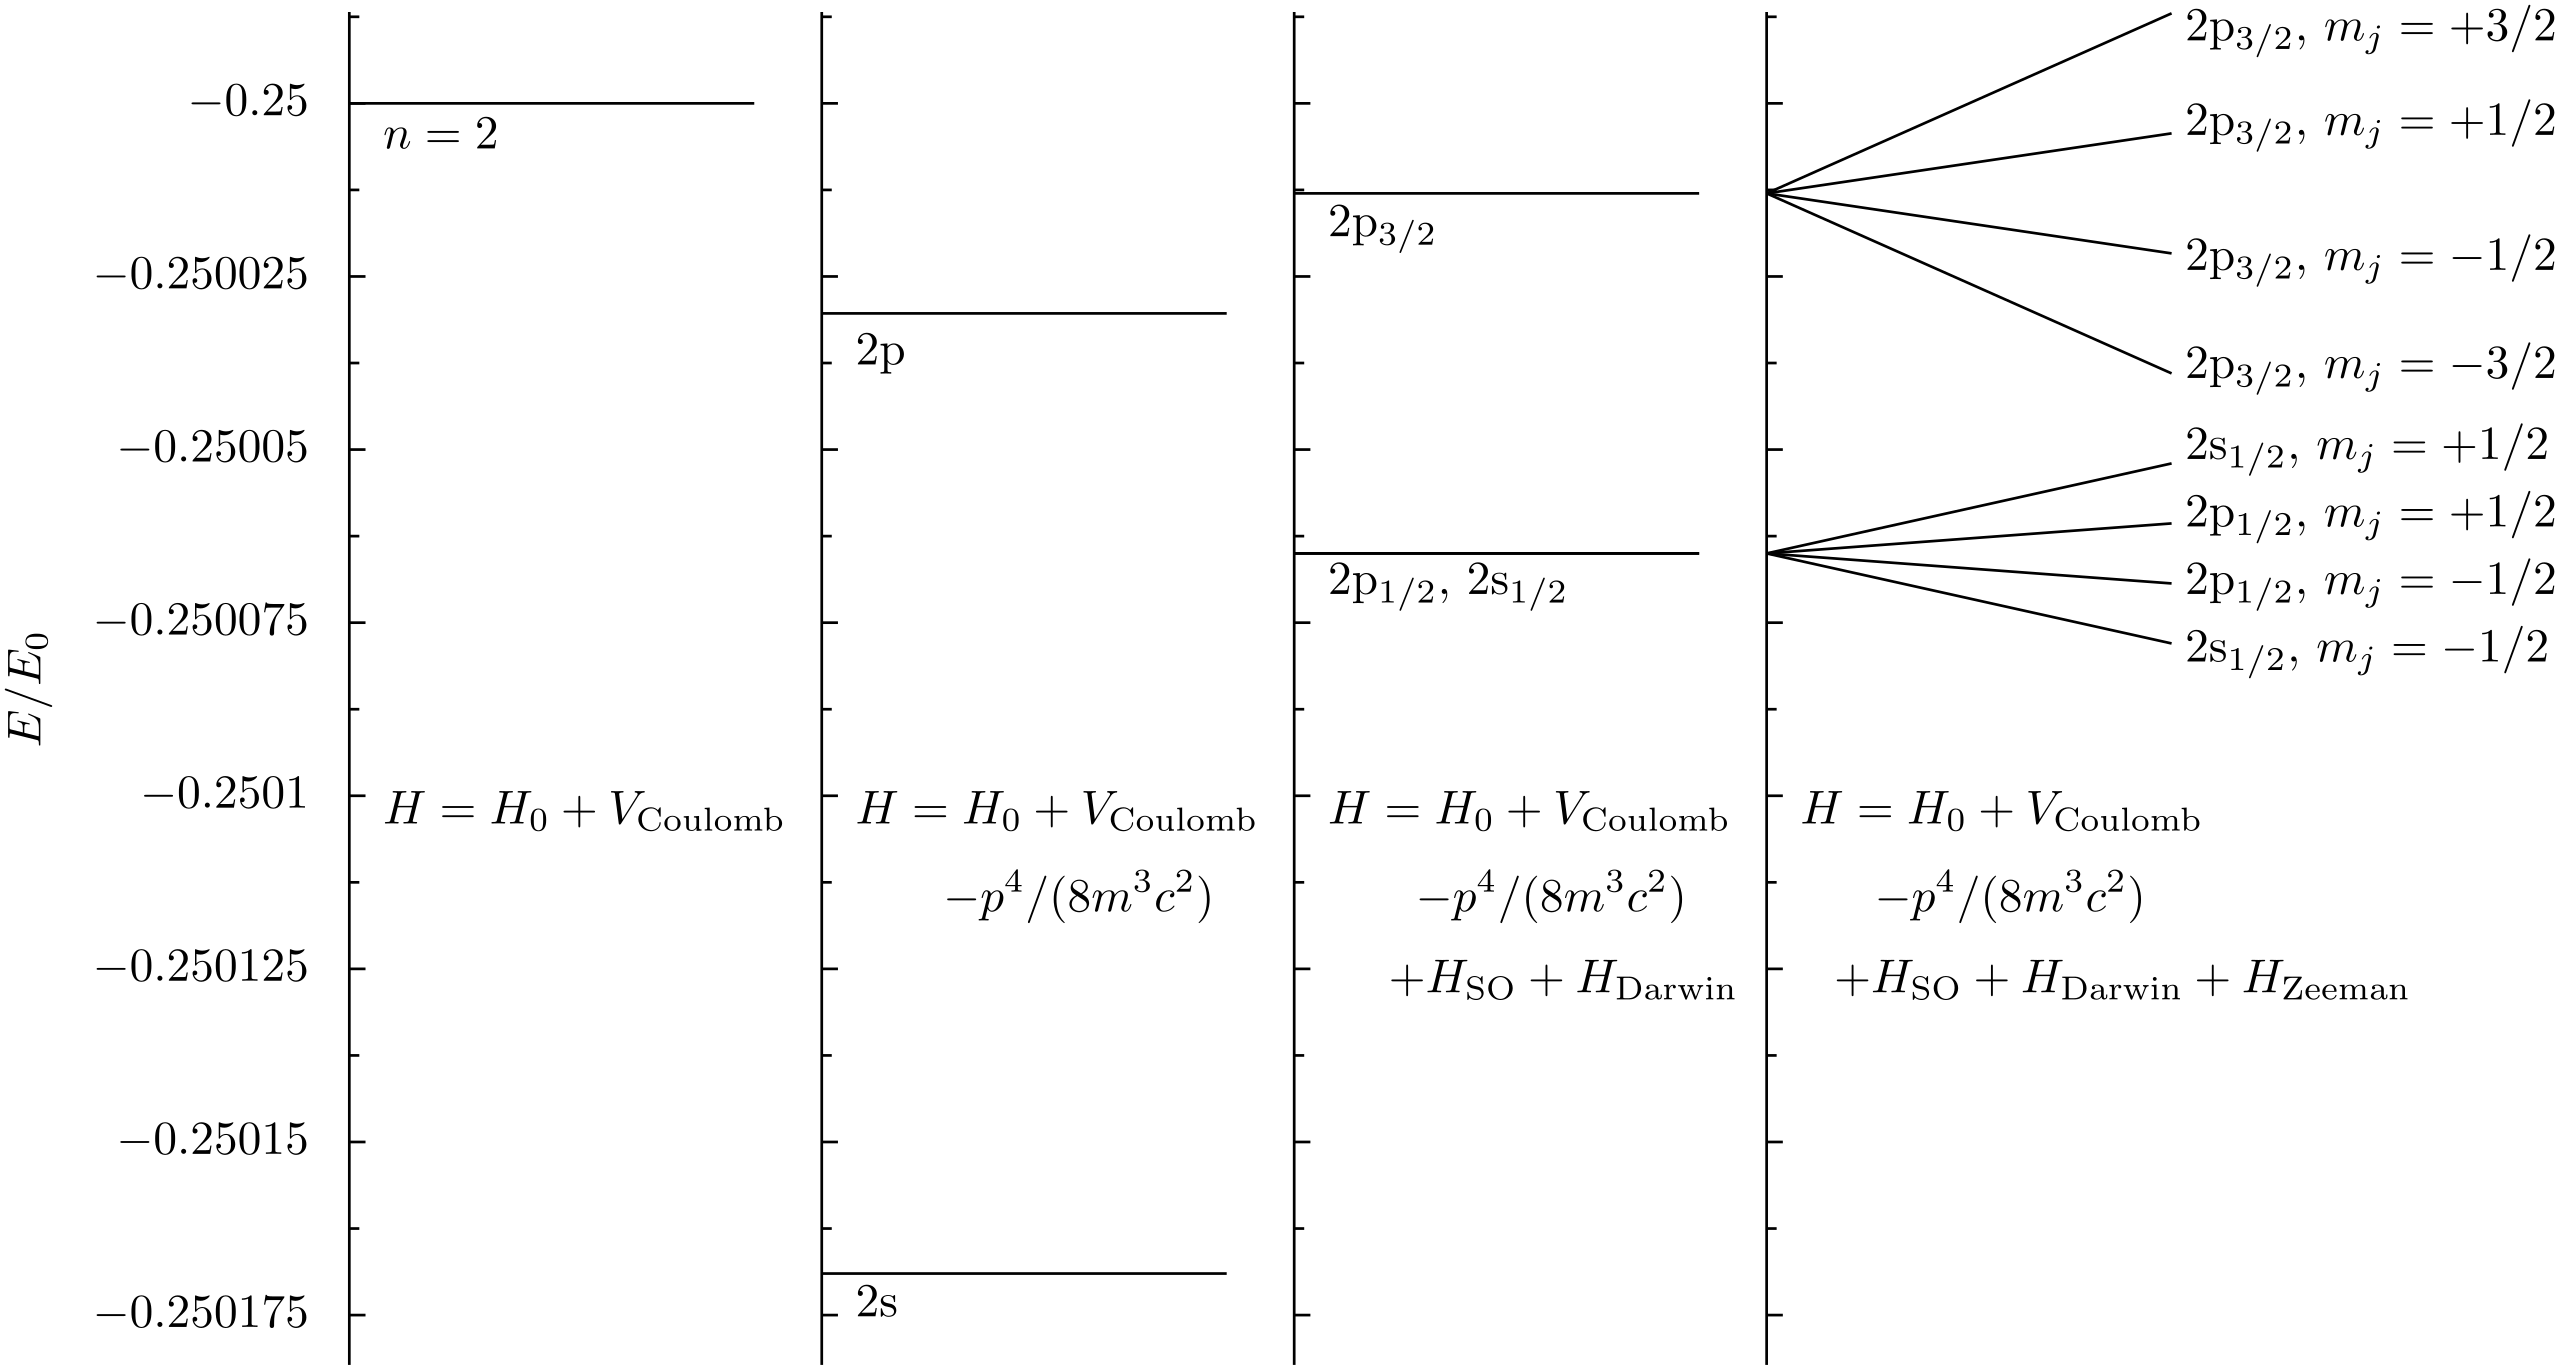
\includegraphics[width=\linewidth]{img/2560px-Hydrogen_fine_structure_energy_2.png}
    \caption{Visualisierung einiger Korrekturen der Feinstruktur bei Wasserstoff.
    Der Lamb-Shift ist hier noch nicht berücksichtigt.
    \refimgsource{Wikimedia}{https://commons.wikimedia.org/wiki/File:Hydrogen_fine_structure_energy_2.svg}{22.02.2022}{public domain}}
    \label{fig:feinstruktur wasserstoff}
\end{figure}

\begin{fquestion}{Woher weiß man, dass $2\mathrm{p}_{1/2}$ eine niedrigere Energie als $2\mathrm{p}_{3/2}$ hat?}
    Man kann ein externes Magnetfeld anlegen, um die Zustände unterscheiden zu können.
    Dabei spaltet sich $2\mathrm{p}_{3/2}$ in 4 Niveaus, und $2\mathrm{p}_{1/2}$ nur in 2 Niveaus auf.
\end{fquestion}

\begin{fquestion}{Strahlungskorrekturen veranschaulichen durch Zitterbewegung des Elektrons und Vakuumfluktuation?}
    (siehe Povh, Streuung und Strukturen, 4.1.3 und 4.2)
    
    \emph{Zitterbewegung}: Das Elektron ist nicht genauer als seine Compton-Wellenlänge $\Bar{\lambda}_e = \frac{\hbar}{m_ec}$ lokalisierbar.
    Das Potential wird dadurch verschmiert, was man über eine Unsicherheit $\delta\Vec{r}$ beschreiben kann.
    Da keine Richtung bevorzugt ist, folgt dann
    $$ V(\Vec{r} + \delta\Vec{r}) \equiv V(r) + \frac{1}{2} \frac{\nabla^2}{3}V(r) \langle (\delta\Vec{r})^2 \rangle  + \mathcal{O}(\delta\Vec{r}^4). $$
    Dabei gilt $\nabla^2 V(r) = 4\pi\alpha \delta (\Vec{r})$, die Korrektur ist also nur für S-Zustände relevant.
    Man erhält also das Störpotential $V_Z = \frac{2\pi \alpha}{3m_e^2} \delta (\Vec{r})$ (Im Erwartungswert gilt dann $\delta \rightarrow |\psi(0)|^2$).
    \\
    \emph{Lamb-Shift}: Es tragen zwei sogenannte Strahlungskorrekturen bei, Polarisation des Vakuums und Vakuumfluktuationen.
    Letztere liefert den Hauptbeitrag, man betrachtet den Einfluss der Fluktuation von $\Vec{E}$ auf $\delta \Vec{r}$.
    Genau wie bei der Zitterbewegung erhält man wieder über denselben Taylor-Ansatz eine Abschätzung der Korrektur.
    Allerdings ist die Herleitung der Vakuumfluktuation von $\Vec{E}$ etwas aufwendiger.
    Das Endergebnis im Povh ist 
    $$\Delta E_n = -E_n \frac{8\pi\alpha^3}{3n} \log \left( \frac{1}{\alpha^2} \right) > 0.$$
\end{fquestion}

\begin{fquestion}{Was passiert mit externem Magnetfeld, also Zeeman-Effekt?}
    Die Energieniveaus sind durch 
    $$\Delta E = -\Vec{\mu}\cdot\Vec{B}$$
    gegeben.
    Dabei kann man im schwachen Magnetfeld annehmen, dass $\Vec{L}$ und $\Vec{S}$ zum Gesamtdrehimpuls $\Vec{J}$ koppeln.
    Dann gilt
    $$\Vec{\mu} \simeq -\mu_Bg_J\frac{\Vec{J}}{\hbar}$$
    mit $\Vec{\mu}_J = g_L\Vec{\mu}_L + g_S\Vec{\mu}_S$ ($g_L = 1$ und $g_S \approx 2$).
    Der Lande-Faktor $g_J$ ist über
    $$\Vec{\mu}_J =: g_J\mu_B\Vec{J}$$
    definiert.
    Insbesondere ist also $g_J\Vec{J} = g_L\Vec{L} + g_S\Vec{S}$.
    Man kann zeigen, dass
    $$g_J = g_L \frac{J(J+1) + L(L+1) - S(S+1)}{2J(J+1)} + g_S \frac{J(J+1) - L(L+1) + S(S+1)}{2J(J+1)}.$$
    Betrachte dazu $\expval{\Vec{\mu}_J\cdot\Vec{J}} = g_J\mu_B\hbar^2 J(J+1)$ und andererseits
    $$g_J\expval{\Vec{J}\,^2} = \expval{g_L\Vec{L}\cdot\Vec{J} + g_S\Vec{S}\cdot\Vec{J}}, $$
    wobei $2\Vec{L}\cdot\Vec{J} = -(\Vec{J}-\Vec{L})^2 + \Vec{J}^2 + \Vec{L}^2 = \Vec{J}^2+\Vec{L}^2 - \Vec{S}^2$ (analog für den anderen Term).
    
    Qualitativ spaltet sich also $2p_{3/2}$ in $2J + 1 = 2\cdot \frac{3}{2} + 1 = 4$ Niveaus auf.
    Da $\Delta E = g_Jm_J\mu_B B$ haben Zustände mit höherem $m_J$ mehr Energie.
\end{fquestion}

\begin{fquestion}{Wann ist LS-Kopplung, wann jj-Kopplung relevant?}
    Grundsätzlich können wir den Hamiltonian als 
    $$H \equiv H_0 + \beta\frac{\expval{\Vec{L}\cdot\Vec{S} }}{r^3} + \gamma \Vec{J}\cdot\Vec{B}$$
    auffassen, wobei $\beta,\gamma$ hier irrelevante Vorfaktoren sind.
    Das Coulomb-Potential sei in $H_0$ enthalten, die anderen Terme modellieren dann jeweils die Spin-Bahn-Kopplung und die Wirkung eines externen Magnetfeldes.
    \\
    Ohne $\Vec{B}$-Feld und LS-Term wissen wir, dass die Eigenzustände durch $|nlm_lm_s\rangle$ beschrieben werden können.
    Unter Berücksichtigung der Spin-Bahn-Kopplung verwendet man stattdessen $|njm_j\rangle$.
    Solange der Zeeman-Term klein ist (also kleine $\Vec{B}$-Felder), können wir weiterhin $m_j$ als gute Quantenzahlen verwenden.
    Für große Felder ist der LS-Term dann vernachlässigbar, weshalb $m_l$ und $m_s$ wieder ``gute'' Quantenzahlen sind.
    Analog kann man durch den Vergleich von LS-Term und $H_0$ auch argumentieren, dass für leichte Atome LS-Kopplung vorliegt.
\end{fquestion}

\begin{fquestion}{Was passiert bei sehr hohen Magnetfeldern?}
    Entspricht dem Paschen-Back-Effekt, $L$ und $S$ koppeln nicht mehr.
    Die Energien sind jetzt $\Delta E = (g_lm_l + g_sm_s)\mu_B B$, da der Zeeman-Term den LS-Term dominiert.
\end{fquestion}

\begin{fquestion}{Was passiert bei dem Übergang von niedrigen zu hohen Feldern?}
    Für bestimmte Niveaus gibt es vermiedene Niveaukreuzungen (= AVL, avoided level crossing).
    Voraussetzung dafür ist, dass die Zustände ``dieselbe Symmetrie'' besitzen.
    Dann können sie mischen, und die Kreuzung vermeiden.
    Konkret bedeutet das, dass sich das $2\mathrm{p}_{3/2}$-Niveau mit $m_J = -\frac{3}{2}$ und das $2\mathrm{p}_{1/2}$-Niveau mit $m_J = \frac{1}{2}$ kreuzen, nicht aber das $2\mathrm{p}_{3/2}$-Niveau mit $m_J = -\frac{1}{2}$ und das $2\mathrm{p}_{1/2}$-Niveau mit $m_J = \frac{1}{2}$.
    Im letzteren Fall gilt $m_l = -1$ und $m_s = \frac{1}{2}$, bzw. $m_l = 1$ und $m_s = -\frac{1}{2}$ (siehe \autoref{fig:zeeman wasserstoff}).
    Für beide Kombinationen ist $m_l + 2m_s = 0$.
\end{fquestion}

\begin{figure}[!ht]
    \centering
    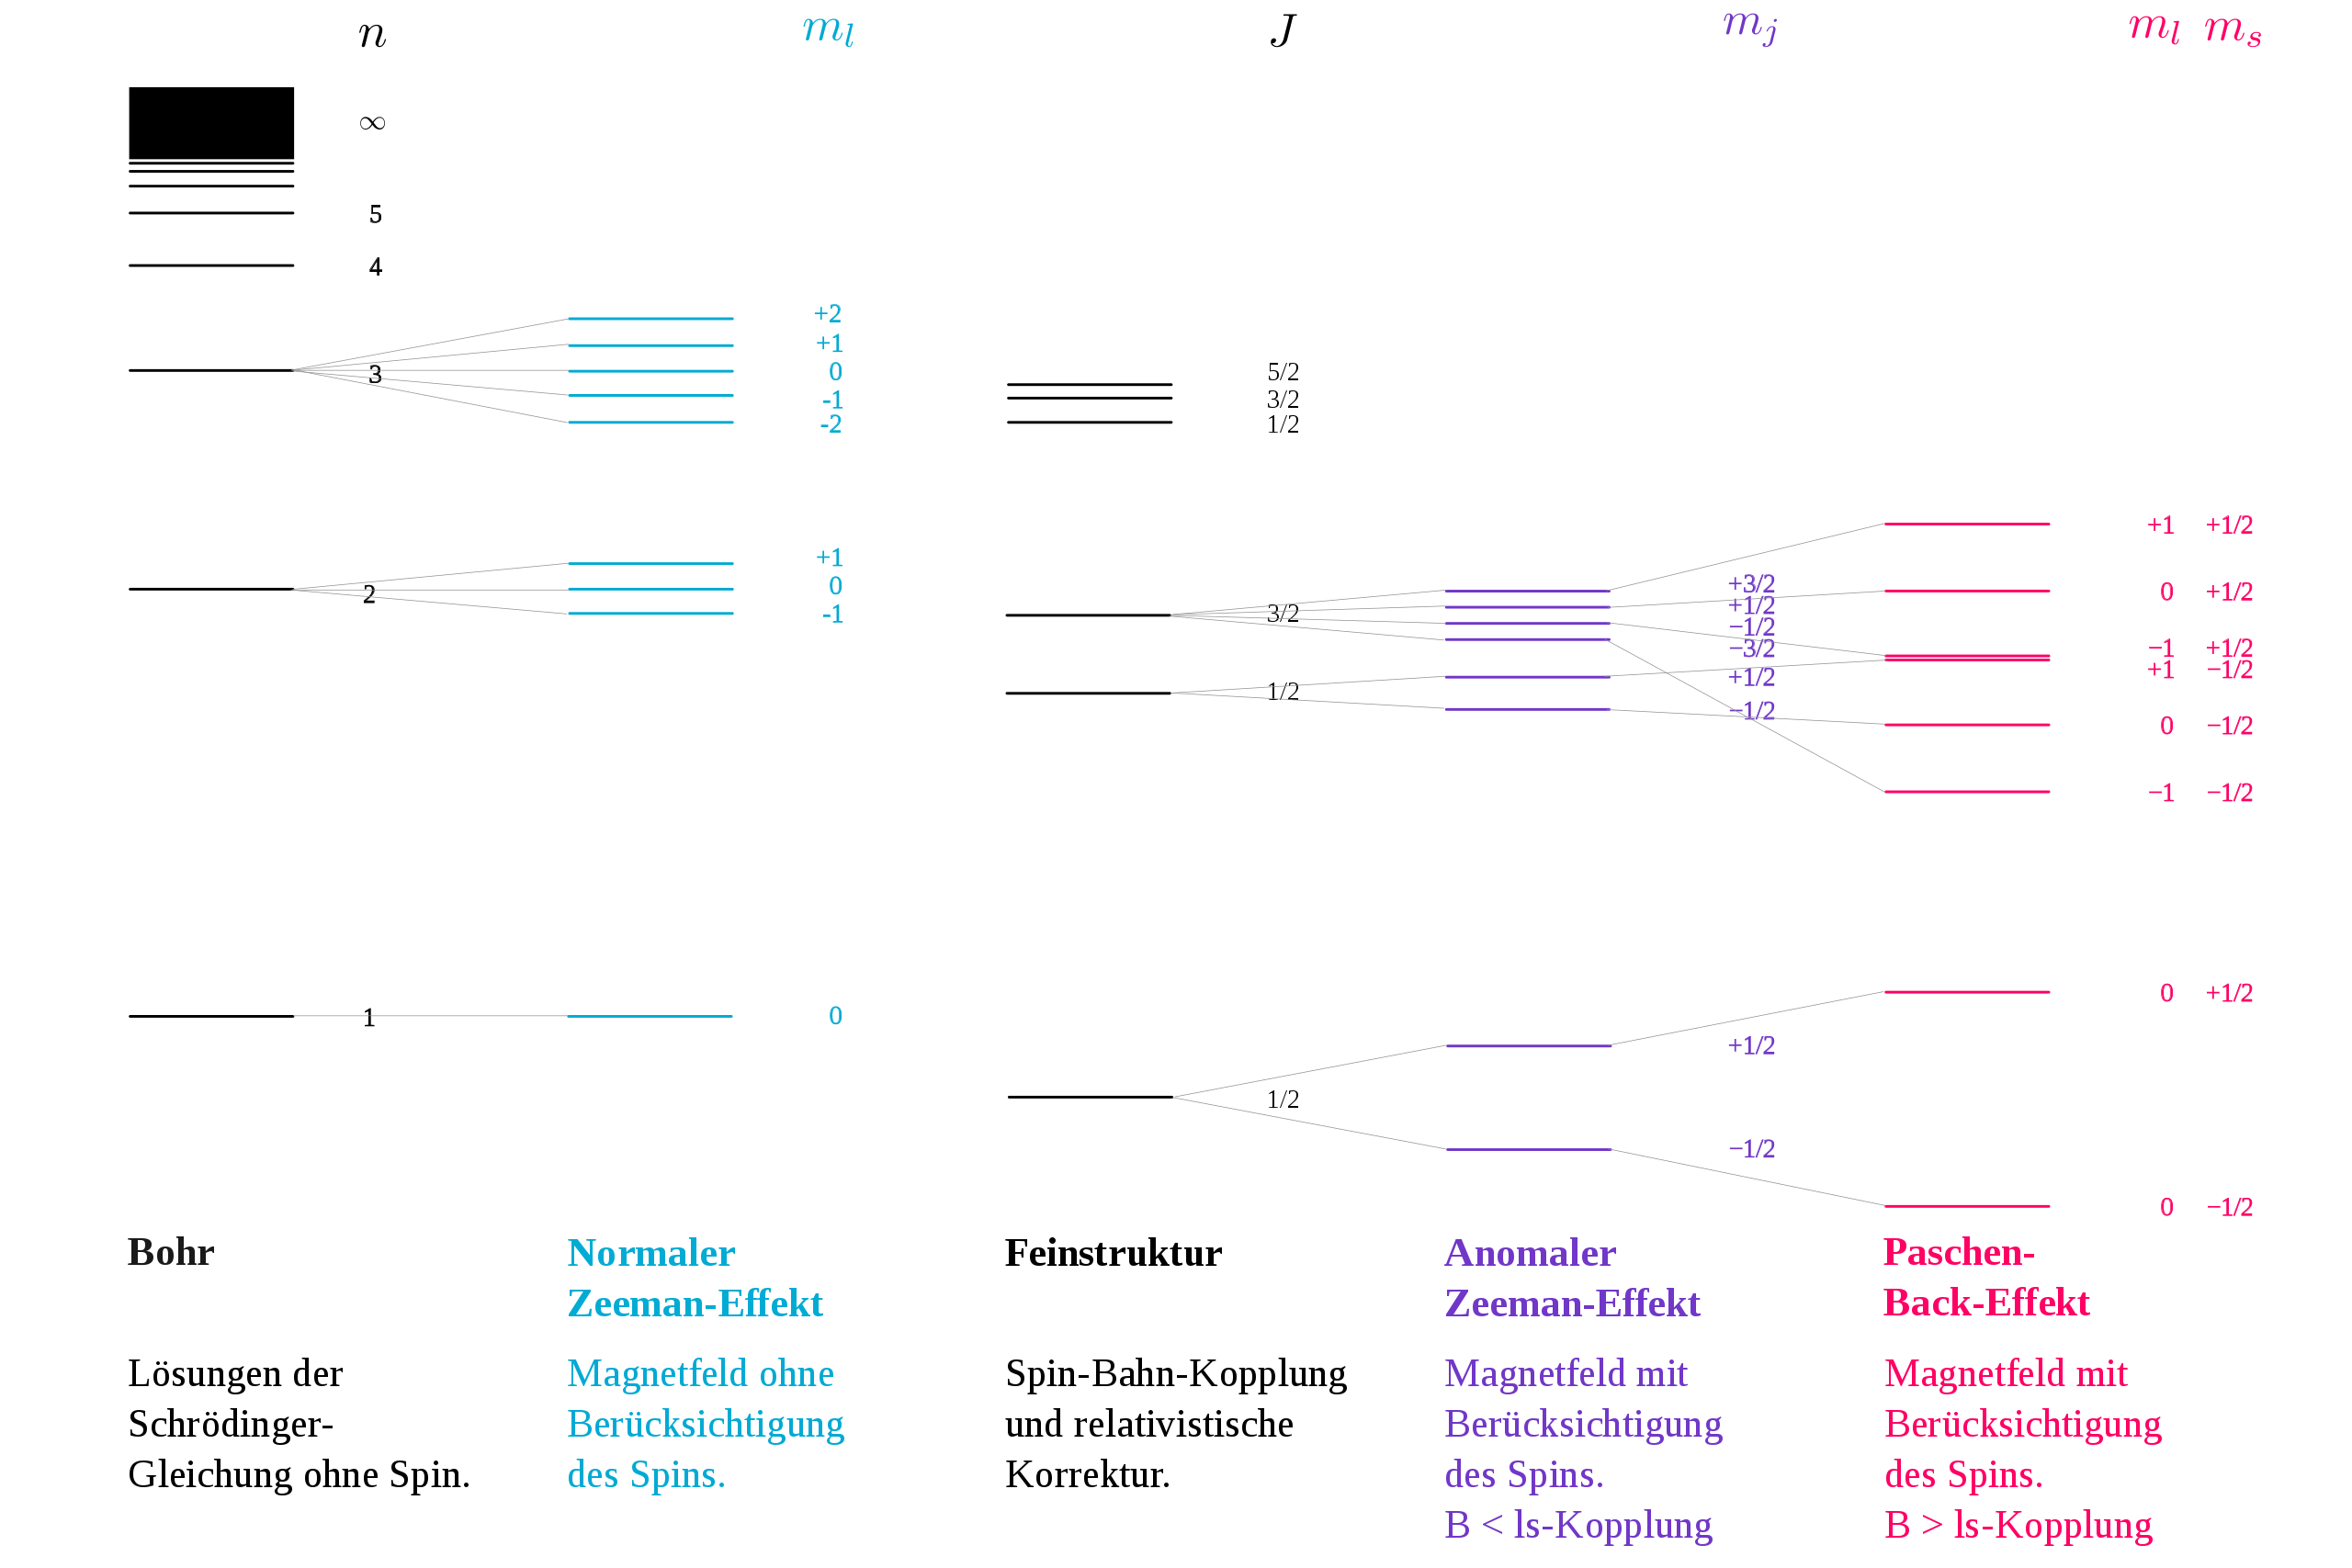
\includegraphics[width=\linewidth]{img/Wasserstoff_Zeeman.png}
    \caption{Aufspaltung der Energie-Niveaus von Wasserstoff in einem externen Magnetfeld (Zeeman-Effekt).
    \refimgsource{Wikimedia}{https://commons.wikimedia.org/wiki/File:Wasserstoff_Zeeman.svg}{22.02.2022}{public domain}}
    \label{fig:zeeman wasserstoff}
\end{figure}

% \begin{question}{Bei welchen Niveaus passiert das?}
%     $m_J = \pm\frac{3}{2}$ kreuzen sich, nur AVL für $m_J = \pm\frac{1}{2}$ ???
%     diese zwei Zustände vermeiden die Kreuzung, da für sie $m_l + 2m_s = 0$, sie wären also ohne Kopplung entartet ??? 
%     Kopplung fällt nur bei unendlichen Magnetfeldern weg, also Kreuzungspunkt im Unendlichen ???
% \end{question}

% \begin{question}{Wie kann man das mit AVL erklären?}
%     Die Zustände, die AVL machen, nähern sich so weit, dass sie nicht mehr zu unterscheiden sind
% \end{question}

\begin{fquestion}{Welche Größenordnung hat die Feinstruktur?}
    $E_{FS} \sim E_n \alpha^2 \sim \alpha^4$.
    $E_n$ in eV-Bereich, also $E_{FS}$ in meV-Bereich.
\end{fquestion}

\begin{fquestion}{Wie sieht das bei Atomkernen aus?}
    $E_n$ in MeV.
    Da $\alpha_s \sim 0.1-1$, liegt $E_{FS}$ auch im MeV-Bereich.
\end{fquestion}

\begin{fquestion}{Was hat das für Auswirkungen?}
    Dass die Feinstruktur in der gleichen Größenordnung wie die primäre Energieskala liegt hat eine starke Durchmischung der Energieniveaus zur Folge. 
    Um die magischen Zahlen vollständig zu erklären, muss die Feinstruktur berücksichtigt werden. 
    Zum Beispiel sorgt die Absenkung des $2f_{7/2}$ Niveaus für die magische Zahl 28. 
\end{fquestion}

% \begin{question}{Was gibt es denn noch für Quantenzahlen außer n?}
%     $l, s, m_l$ und $m_s$
% \end{question}

% \begin{question}{Warum sind $B$ und $L$ denn proportional, und wie?}
    
% \end{question}

\begin{fquestion}{Wie sieht das alles bei Mesonen aus, z.B. Charmonium?}
    Das Potential der starken Wechselwirkung kann hier als $V(r) = -\frac{4}{3} \frac{\alpha_s}{r} + kr$ angenommen werden, wobei $\alpha_s = \alpha_s(2m_\mathrm{charm}^\mathrm{const}) \approx 0.2$ mit der Konstituentenmasse $m_\mathrm{charm}^\mathrm{const} = \SI{1.5}{GeV}$.
    Für eine Abschätzung der Grundzustandsenergie kann man $k\simeq 0$ annehmen.
    Dann ist in Analogie zum Wasserstoff $E_0\approx \frac{\mu }{2}\left(\frac{4\alpha_s}{3} \right)^2 \approx \SI{27}{MeV} $, wobei $\mu = \frac{m_\mathrm{charm}^\mathrm{const}}{2}$ die reduzierte Masse ist (exp. Wert ist $\SI{32}{MeV}$, bei einer Gesamtmasse $\eta_\mathrm{charm}(1\mathrm{S} ) = \SI{2980}{MeV}$).
    
    In dieser Näherung wäre die maximale Masse $2m_\mathrm{charm}^\mathrm{const} = \SI{3}{GeV}$.
    Tatsächlich hat aber bereits der erste angeregte Zustand eine Masse von $\eta_\mathrm{charm}(2\mathrm{S} ) = \SI{3640}{MeV}$, was schematisch mit dem zusätzlichen linearen Term erklärt werden kann (Bindungszustände beliebig hoher Energie).
    
    % Grobstruktur erklären, Größenordnung $E_0$ mit $m_\text{charm}$ abschätzen ??? 
    % starke WW, also noch linearen Term im Potential für Confinement
\end{fquestion}

\begin{fquestion}{Woher kommt der Faktor $\frac{4}{3}$?}
    Es gibt drei Farbladungen und damit zunächst 9 mögliche effektive Gluonen
    $$|\mathrm{r}\overline{\mathrm{g}}\rangle, |\mathrm{r}\overline{\mathrm{b}}\rangle, |\mathrm{g}\overline{\mathrm{r}}\rangle, |\mathrm{g}\overline{\mathrm{b}}\rangle, |\mathrm{b}\overline{\mathrm{r}}\rangle, |\mathrm{b}\overline{\mathrm{g}}\rangle,
    |\mathrm{r}\overline{\mathrm{r}}\rangle,
    |\mathrm{g}\overline{\mathrm{g}}\rangle,
    |\mathrm{b}\overline{\mathrm{b}}\rangle.$$
    Da keine langreichweitige starke Wechselwirkung beobachtet wurde, kann es aber keines der farbneutralen Gluonen geben.
    Formal schließt man das ``weiße'' Gluon mit $\frac{1}{\sqrt{3}} (|\mathrm{r}\overline{\mathrm{r}}\rangle + |\mathrm{g}\overline{\mathrm{g}}\rangle + |\mathrm{b}\overline{\mathrm{b}}\rangle)$ aus.
    Üblicherweise werden die übrigen 8 Gluonen der SU(3) dann über 
    $$\begin{aligned} |\lambda_1\rangle &= \frac{1}{\sqrt{2}} (|\mathrm{r}\overline{\mathrm{b}}\rangle + |\mathrm{b}\overline{\mathrm{r}}\rangle ),&&&
    |\lambda_2\rangle &= \frac{-\i}{\sqrt{2}} (|\mathrm{r}\overline{\mathrm{b}}\rangle - |\mathrm{b}\overline{\mathrm{r}}\rangle ),\\
    |\lambda_3\rangle &= \frac{1}{\sqrt{2}} (|\mathrm{r}\overline{\mathrm{g}}\rangle + |\mathrm{g}\overline{\mathrm{r}}\rangle ),&&&
    |\lambda_4\rangle &= \frac{-\i}{\sqrt{2}} (|\mathrm{r}\overline{\mathrm{g}}\rangle - |\mathrm{g}\overline{\mathrm{r}}\rangle ),\\
    |\lambda_5\rangle &= \frac{1}{\sqrt{2}} (|\mathrm{b}\overline{\mathrm{g}}\rangle + |\mathrm{g}\overline{\mathrm{b}}\rangle ), &&&
    |\lambda_6\rangle &= \frac{-\i}{\sqrt{2}} (|\mathrm{b}\overline{\mathrm{g}}\rangle - |\mathrm{g}\overline{\mathrm{b}}\rangle ),\\
    |\lambda_7\rangle &= \frac{1}{\sqrt{2}} (|\mathrm{r}\overline{\mathrm{r}}\rangle - |\mathrm{b}\overline{\mathrm{b}}\rangle ),&&&
    |\lambda_8\rangle &= \frac{1}{\sqrt{6}} (|\mathrm{r}\overline{\mathrm{r}}\rangle +  |\mathrm{b}\overline{\mathrm{b}}\rangle - 2|\mathrm{g}\overline{\mathrm{g}}\rangle ) \end{aligned}$$
    dargestellt (siehe Gell-Mann-Matrizen $\lambda_{1\dots 8}$, die Indizierung ist manchmal anders). 
    Die ``hand-wavy'' Erklärung für den Faktor ist dann 
    $$\frac{1}{2} \Bigg[ \bigg\vert \underbrace{\frac{1}{\sqrt{2}}}_{|\lambda_1\rangle} \bigg\vert^2 + \bigg\vert \underbrace{\frac{-\i}{\sqrt{2}}}_{|\lambda_2\rangle} \bigg\vert^2 \Bigg] + \frac{1}{2} \Bigg[ \bigg\vert \underbrace{\frac{1}{\sqrt{2}}}_{|\lambda_3\rangle} \bigg\vert^2 + \bigg\vert \underbrace{\frac{-\i}{\sqrt{2}}}_{|\lambda_4\rangle} \bigg\vert^2 \Bigg] + \frac{1}{2} \Bigg[ \bigg\vert \underbrace{\frac{1}{\sqrt{2}}}_{|\lambda_7\rangle} \bigg\vert^2 + \bigg\vert \underbrace{\frac{1}{\sqrt{6}}}_{|\lambda_8\rangle} \bigg\vert^2 \Bigg] = \frac{4}{3}. $$
    Konzeptionell korrespondieren die Terme zu Feynman-Diagrammen, wo man üblicherweise die Betragsqudrate der Amplituden addiert. 
    % Die $\frac{1}{2}$-Faktoren sind jeweils von $\alpha_s$ abgespalten ??? 
    % Hier sind die Terme ausgehend von einem ursprünglich roten Quark aufgeschrieben.
    % ??? Wie sieht das in einem Feynman-Diagramm aus? 
    % Die Gluonen von oben existieren ja gar nicht, man zeichnet doch immer etwas wie rot-anti-blau ein etc. ??? 
    % ??? Wie kommt man damit jetzt auf die ``Rechnung'' aus der Vorlesung
\end{fquestion}

\begin{fquestion}{Was passiert bei kleinen Abständen?}
    Der lineare Term ist vernachlässigbar, man kann das Potential wieder (grob) als $\frac{1}{r}$-Potential ansehen und analog zum Coulomb-Potential vorgehen.
\end{fquestion}

\begin{fquestion}{Was passiert bei großen Abständen? }
    Der lineare Term führt zu einer beliebig großen Energie, bis genug für die Quark-Antiquark-Paarbildung vorhanden ist.
    Das erklärt dann phänomenologisch das Confinement, weil sich zwei Quarks nur so weit entfernen können, bis die Paarbildung auftritt.
    Es treten also nie ``isolierte'' Quarks auf.
\end{fquestion}

\begin{fquestion}{Welcher Effekt führt hier eigentlich zur Feinstruktur?}
    % starker Isospin ???  
    Die Aufspaltung der P-Zustände kann analog zum Wasserstoff-Atom über die Spin-Bahn-Kopplung erklärt werden.
    (siehe Povh 14.3, Quark-Antiquark-Potential)
\end{fquestion}

\begin{fquestion}{Was passiert bei der Hyperfeinstruktur?}
    Der Gesamtdrehimpuls $\Vec{J}$ koppelt an den Kernspin $\Vec{I}$ zum Gesamtspin $\Vec{F}$.
    Es dominieren zwei Effekte, die Kopplung des magnetischen Kernmomentes an das Magnetfeld des Elektrons, sowie das elektrische Quadrupolmoment des Kerns.
\end{fquestion}

\begin{fquestion}{Wie sieht die Kopplung des Kernmomentes aus?}
    Das Kernmoment ist $\Vec{\mu}_I = g_I\mu_N \Vec{I}$, mit dem Kernmagneton $\mu_N = \frac{e\hbar}{2m_p}$.
    
    Das Magnetfeld des Elektrons besteht aus einem Beitrag vom Bahndrehimpuls
    $$\Vec{B}_L = \frac{\mu_0}{4\pi r^3} 2\Vec{\mu}_L$$
    und einem Beitrag vom Spin durch $\Vec{A}_S = -\frac{\mu_0\Vec{\mu}_S}{4\pi} \times \nabla\frac{1}{r}$, also
    $$\Vec{B}_S = \nabla\times\Vec{A}_S = \frac{\mu_0}{4\pi r^3} \big[ 3(\Vec{\mu}_S\cdot \Vec{e}_r)\Vec{e}_r - \Vec{\mu}_S \big] + \frac{2\mu_0}{3}\Vec{\mu}_S\delta (\Vec{r}).$$
    (Der Faktor $\frac{2}{3}$ ergibt sich aus der Formel für das homogene Magnetfeld in einer Kugel oder einer rotierenden Kugel mit Oberflächenladung).
    
    Der distributionelle Anteil ist dabei nur für S-Zustände relevant, also für $L=0$.
    Die Energieänderung ist dann $\Delta E = -\Vec{\mu}_I \cdot (\Vec{B}_L + \Vec{B}_S)$.
\end{fquestion}

\begin{fquestion}{Gibt es die Hyperfeinstruktur auch nur für angeregte Zustände, wie bei der Feinstruktur und z.B. 2p?}
    Nein, gibt es auch bei $s_{1/2}$.
    Ein prominentes Beispiel ist die 21\,cm-Linie von Wasserstoff (entspricht 1420\,MHz).
    
    Allgemein gilt für Zustände mit $L=0$ näherungsweise eine vereinfachte Energiekorrektur.
    Diese ist
    $$\Delta E_\mathrm{HFS} \simeq \frac{2}{3} \expval{\Vec{\mu}_1\cdot\Vec{\mu}_2} |\psi (0)|^2 \equiv a \expval{\Vec{s}_1\cdot\Vec{s}_2},$$
    wobei $\Vec{\mu}_k = g_k \frac{g_\mathrm{int}}{2m_k} \Vec{s}_k$.
    Hierbei ist $g_\mathrm{int} = \sqrt{4\pi \alpha_\mathrm{int}}$ die Ladung der relevanten Wechselwirkung (für EM beispielsweise ist $g_\mathrm{int} \approx 0.3$).
    Mit $|\psi(0)|^2 = \frac{1}{\pi n^3r_0^3}$ und $r_0 = \frac{1}{m_\mathrm{red} \alpha_\mathrm{int}}$ findet man dann
    $$a = \frac{2}{3n^2} g_1g_2 \alpha_\mathrm{int}^4 \frac{m_\mathrm{red}^3}{m_1m_2}.$$
    
    Für das Elektron ist $g_s\approx 2$, für das Proton $g_s \approx 5.6$.
    In dieser Näherung findet ist $a \approx \SI{5.89}{\micro eV}$, was mit dem Umrechnungsfaktor $\frac{hc}{e} = \SI{1.24}{eV\,\micro m}$ einer Wellenlänge von
    $$\lambda = \frac{hc}{e}\cdot\frac{1}{a} \approx \SI{21}{cm}$$
    entspricht.
    % Eine höhere Genauigkeit kann man bei dieser Abschätzung nicht erwarten.
\end{fquestion}

\begin{fquestion}{Was ist denn mit dem Erwartungswert des Spin-Produktes passiert?}
    Für Wasserstoff ist $s_{1,2} = \frac{1}{2}$, also ist der Gesamtspin $S=1$ für parallele, und $S=0$ für anti-parallele Ausrichtung.
    Damit gilt 
    $$\langle \Vec{s}_1\cdot\Vec{s}_2\rangle = \frac{S(S+1) - s_1(s_1+1) - s_2(s_2+1)}{2} = \begin{cases} \frac{1}{4}, & \mathrm{parallel} \\ -\frac{3}{4}, & \text{anti-parallel} \end{cases}.$$
    Die Differenz zwischen den Energieniveaus erhält damit also gerade einen Faktor $\frac{1}{4} - \left(-\frac{3}{4}\right) = 1$, womit dann $\Delta E \equiv a$.
\end{fquestion}

\begin{fquestion}{Wie groß ist dann etwa das vom Elektron beim Proton induzierte Magnetfeld?}
    Es gilt $\Delta E \simeq \Vec{\mu}_p \cdot \Vec{B}_\mathrm{ind}$, die gesamte Aufspaltung ist also $a = 2\mu_p B_\mathrm{ind}$ (Differenz zwischen paralleler und anti-paralleler Ausrichtung).
    Damit ist dann 
    $$B_\mathrm{ind} = \frac{a}{2\mu_p} = \frac{a}{2\mu_B g_p} \frac{m_p}{m_e} \approx \SI{16.7}{T}.$$
\end{fquestion}

\begin{fquestion}{Wie beeinflusst ein schwaches externes Magnetfeld die Energieniveaus mit $S=0$ bzw. $S=1$?}
    Es gilt $\Delta E = -\Vec{\mu}_S\cdot\Vec{B}_\mathrm{ext}$, wobei gemäß Wigner-Eckart-Theorem
    $$\Vec{\mu}_S = \frac{\langle\Vec{\mu}_e\cdot\Vec{S} + \Vec{\mu}_p\cdot\Vec{S}\rangle}{\expval{\Vec{S}^2}} \Vec{S} \approx \frac{\langle\Vec{\mu}_e\cdot\Vec{S}\rangle}{S(S+1)} \Vec{S}.$$
    Dabei kann man das magnetische Moment des Protons vernachlässigen.
    Mit $\Vec{S} = \Vec{s}_e + \Vec{s}_p$ folgt daraus dann
    $$\Vec{\mu}_S = g_s\mu_B\Vec{S} \frac{s_e(s_e+1) + \langle\Vec{s}_e\cdot\Vec{s}_p\rangle }{S(S+1)} \approx \mu_B\Vec{S}, $$
    wobei $g_s\approx 2$.
    Damit ändern sich die Energieniveaus dann um $\Delta E \approx \mu_B B_\mathrm{ext} m_S$, mit $m_S=-1,0,1$.
    
    Anmerkung: Bei der Berechnung von $\Vec{\mu}_S$ muss man etwas aufpassen, ausführlich gilt
    $$\begin{aligned} \frac{2 \langle\Vec{s}_e\cdot\Vec{S}\rangle }{ \langle\Vec{S}^2\rangle } &= \frac{2s_e(s_e+1) +  S(S+1) - s_e(s_e+1) - s_p(s_p+1)}{S(S+1)} = \\
    &= \frac{S(S+1)}{S(S+1)}=1,\end{aligned}$$
    wobei auch für anti-parallele Spins $s_e=s_p=\frac{1}{2}$ ist, weshalb $s_e(s_e+1) - s_p(s_p+1) \equiv 0$!
\end{fquestion}

\begin{fquestion}{Wie beeinflusst ein starkes externes Magnetfeld die Energieniveaus mit $S=0$ bzw. $S=1$?}
    Hier koppeln $\Vec{\mu}_e$ und $\Vec{\mu}_p$ näherungsweise unabhängig voneinander an $\Vec{B}_\mathrm{ext}$, da $a$ gegenüber der Aufspaltung vernachlässigbar wird.
    Es gilt dann 
    $$\Delta E = (2\mu_B m_{s_e} - g_p \mu_N m_{s_p}) B_\mathrm{ext},$$ 
    wobei der zweite Term durch $\mu_N \ll \mu_B$ unterdrückt ist.
    Insbesondere ist das Vorzeichen umgekehrt wegen der Ladung des Protons umgekehrt.
\end{fquestion}

\begin{fquestion}{Warum ist die 21\,cm-Linie so interessant?}
    Das ist der Hyperfeinübergang des 1S Wasserstoffniveaus. 
    Bei diesem kommt es zu einem Spinflip, damit ist die Parität erhalten und kein elektrischer Dipolübergang ist möglich. 
    Ein magnetische Dipolübergang ist nötig. 
    Dieser ist unterdrückt. 
    Zudem ist die Photonenergie ca. $\SI{6}{\micro eV}$ und ist damit energetisch unterdrückt. 
    Dieser Zustand hat durch diese Unterdrückung eine Lebensdauer von ca. $11$ Millionen Jahren und eine sehr scharfe Spektrallinie (Lange Lebensdauer $\rightarrow$ scharfer Peak). 
    Daher kann diese Linie zur Vermessung von Geschwindigkeiten von Wasserstoffansammlungen im Universum über den Dopplereffekt benutzt werden. 
\end{fquestion}

\begin{fquestion}{Warum mögen Astrophysiker keine Handys?}
    Handyfrequenzen liegen im Bereich $(0.8 -3.6)\,$GHz und somit im gleichen Frequenzbereich wie der Wasserstoff-Hyperfeinübergang mit $1.420\,$GHz. 
\end{fquestion}

\begin{fquestion}{Woher weiß man bei den Radioteleskopen auf der Erde, dass der Wasserstoff nicht aus der Atmosphäre kommt?}
    Die strahlungslose Abregung durch Stöße ist viel schneller, da Stöße bei irdischen Dichten viel häufiger stattfinden. 
    Daher findet der Hyperfeinübergang hier nicht statt. 
\end{fquestion}

\subsection{Atomkern}

\begin{fquestion}{Was sind die typischen Kernenergien?}
    Typische Bindungsenergien pro Nukleon sind $(7-8)$\,MeV.
    Die Potentialtiefe wächst kontinuierlich von 17\,MeV (Lithium) bis 44\,MeV (Blei) mit der Massenzahl $A$ an.
    Der Fermi-Impuls beträgt etwa 250\,MeV (siehe Povh 6.3).
    Die Energieniveaus wachsen etwa quadratisch (Kastenpotential, also $E_n\sim n^2$).
    Die Fermi-Energien betragen etwa $E_F \approx \frac{p_F^2}{2M} \approx 33$\,MeV (siehe Povh 18.1).
\end{fquestion}

\begin{fquestion}{Wie bestimmt man die Fermi-Energie?}
    Quasieleastische Streuung an Wasser. 
    Über den Abstand des Peaks der im Sauerstoff gebundenen Protonen mit den ``freien'' Protonen kann man die Bindungsenergie bestimmen. 
    Über die Breite des Peaks der gebundenen Protonen kann man den Fermi-Impuls bestimmen, da die Verbreiterung des Peaks durch die Bewegung der Protonen im Kern kommt, diese haben dabei den Fermi-Impuls. 
\end{fquestion}

\begin{fquestion}{Was hat es mit dem Tröpfchenmodell auf sich?}
    Die Bethe-Weizsäcker-Formel lautet
    $$E_B = a_V A - a_O A^{2/3} - a_C \frac{Z^2}{A^{1/3}} - a_A \frac{(N - Z)^2}{A} + \delta(N, Z)$$
    Man betrachtet fünf Beiträge zur Bindungsenergie
    \begin{enumerate}
        \item \emph{Volumenenergie}: $a_VA$, proportional zur Anzahl der Nukleonen $A$.
        Durch die kurze Reichweite der starken Wechselwirkung gibt es keinen $A^2$-Term, den man beispielsweise für die Coulomb-Wechselwirkung erwarten würde.
        Effektiv trägt nur die Wechselwirkung mit nächsten Nachbarn bei.
        \item \emph{Oberflächenenergie}: $-a_OA^{2/3}$, proportional zur Oberfläche des Kerns (also $\propto R^2$).
        Nukleonen an der Oberfläche haben weniger nächste Nachbarn, was zu einer geringeren Bindungsenergie führt.
        \item \emph{Coulombterm}: $-a_C \frac{Z^2}{A^{1/3}}$, proportional zum Quadrat der Anzahl an Protonen.
        Der Faktor $A^{-1/3}$ entspricht der $\frac{1}{R}$-Abhängigkeit.
        \item \emph{Asymmetrieterm}: $-a_A \frac{(N-Z)^2}{A}$ proportional zum Quadrat der Differenz von Neutronen und Protonen. 
        Qualitativ beruht er auf dem Pauli-Prinzip.
        Falls ein Kern deutlich mehr Protonen als Neutronen besitzt, könnte die Energie durch Umwandlung der höher liegenden Neutronen in Protonen verringert werden.
        \item \emph{Paarungsterm}: $\frac{\delta}{A^{1/2}} $ für gg-Kerne, $-\frac{\delta}{A^{1/2}} $ für uu-Kerne und 0 für gu-Kerne (g: gerade, u: ungerade).
    \end{enumerate}
    Die Parameter eines least-squares fit sind etwa $a_V \approx 16\,$MeV, $a_O \approx 18\,$MeV, $a_C \approx 0.7\,$MeV, $a_A \approx 23\,$MeV und $\delta \approx 12\,$MeV.
    Siehe \autoref{fig:experimental-mass-binding-model} für einen Plot der Bindungsenergie pro Nukleon.
\end{fquestion}

\begin{figure}[!ht]
    \centering
    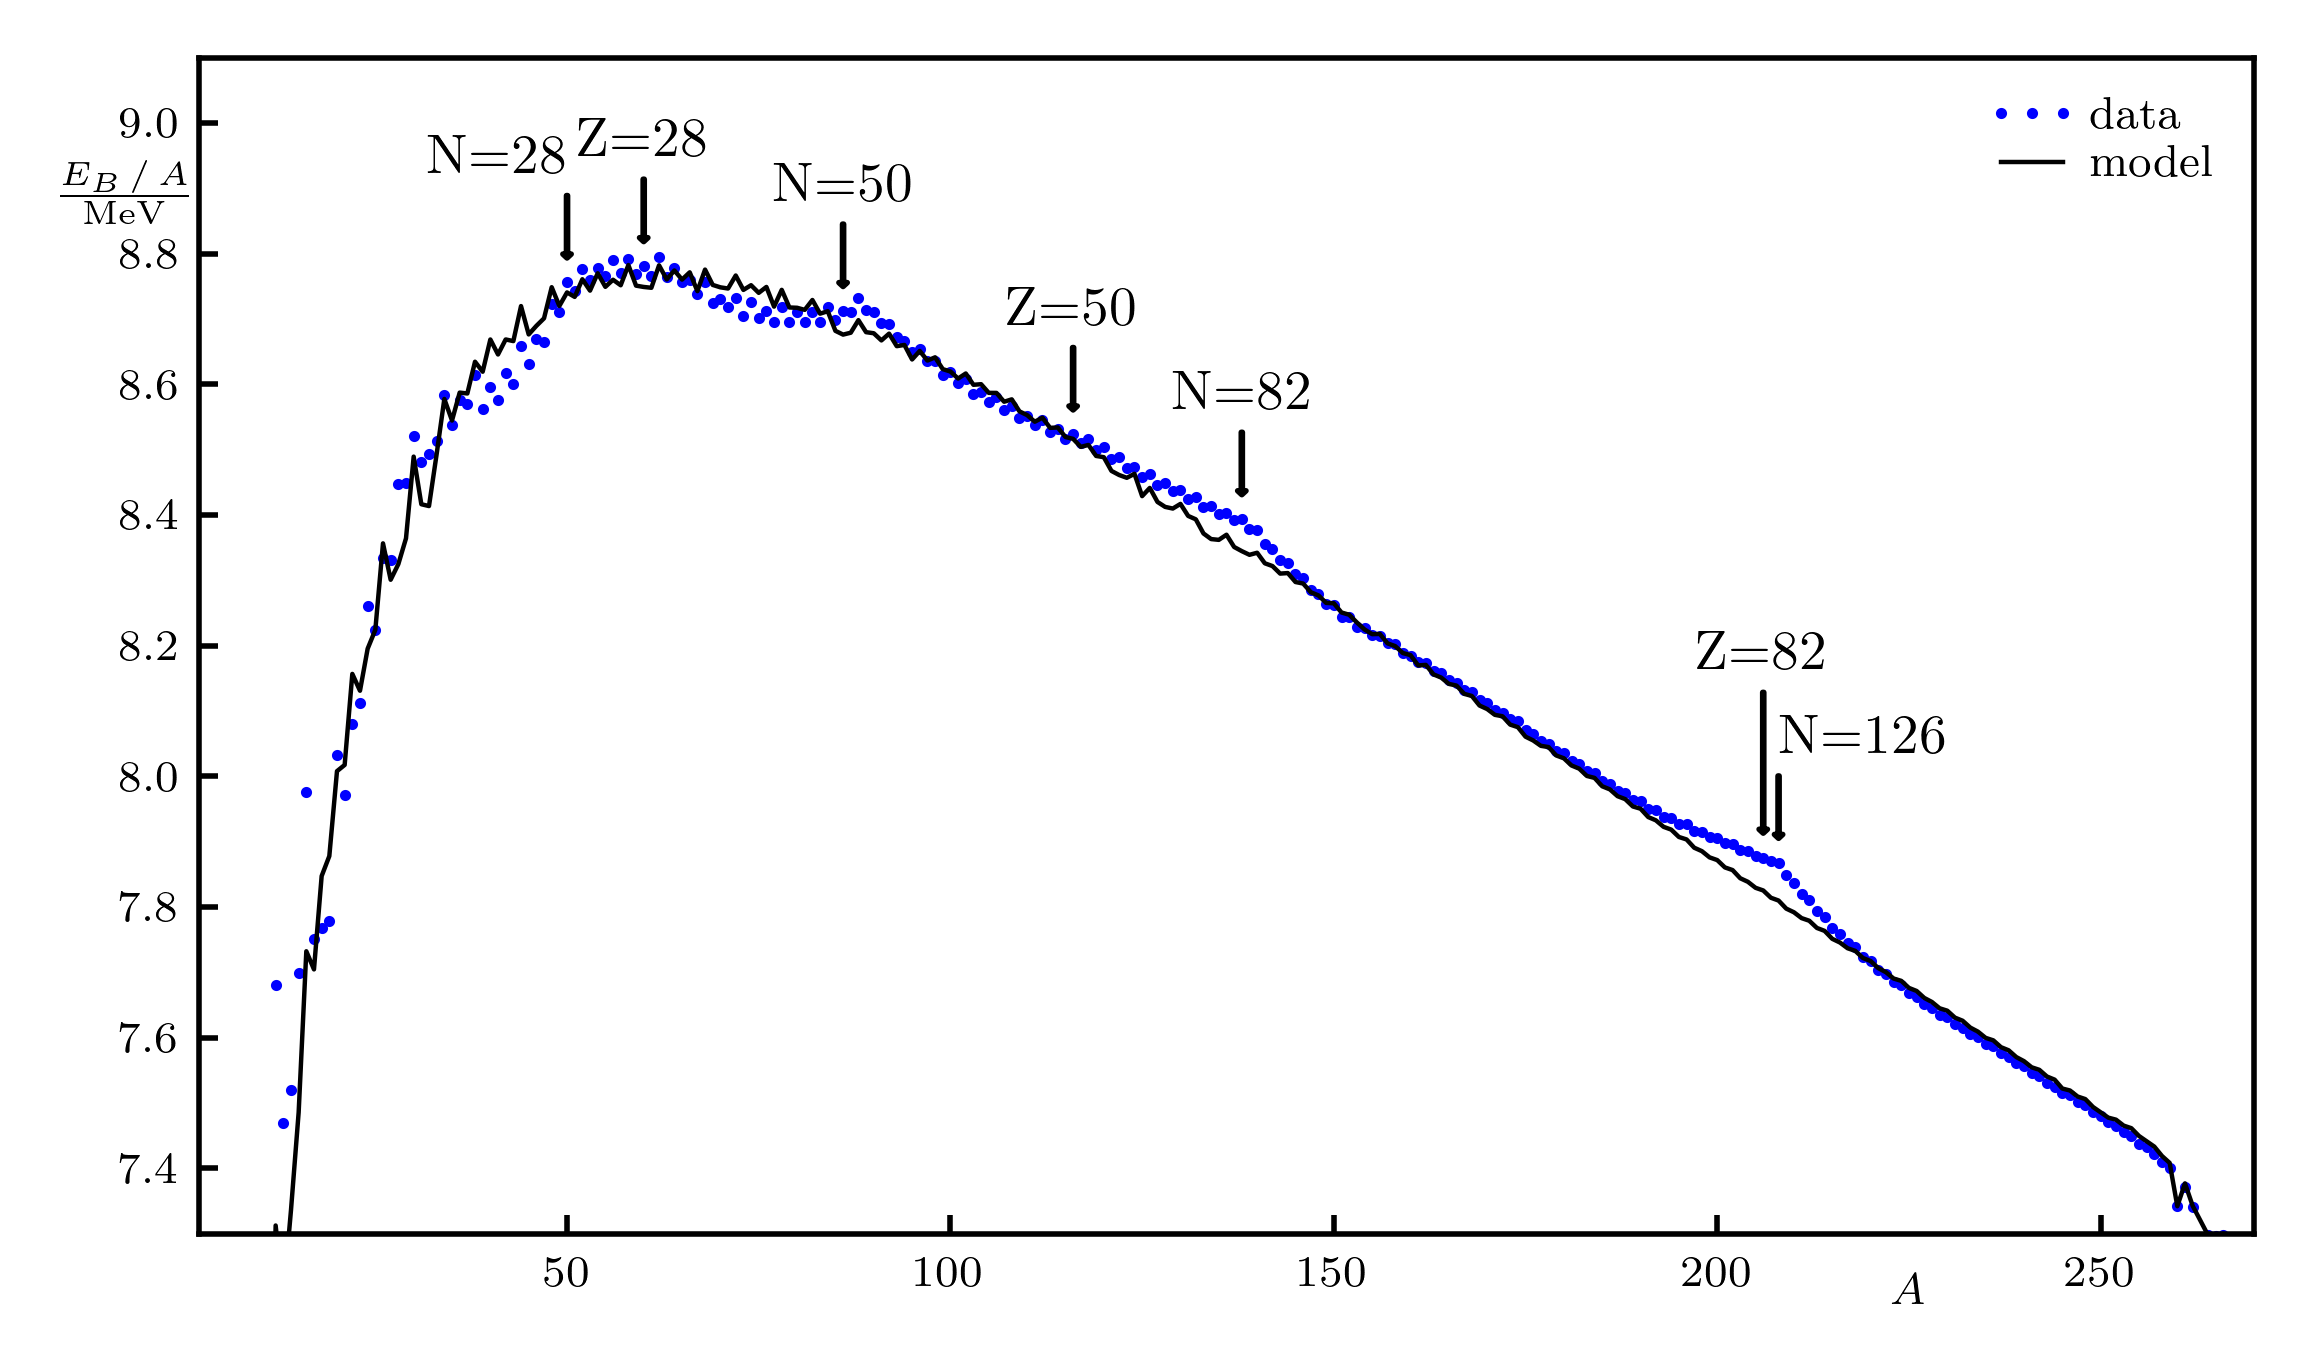
\includegraphics{img/experimental-mass-binding-model2.png}
    \caption{Plot der semi-empirischen Massenformel für $a_V = 15.75\,$MeV, $a_O = -17.8\,$MeV, $a_C = -0.711\,$MeV, $a_A = -23.7\,$MeV und $\delta = 11.18\,$MeV.
    Die experimentellen Daten sind aus \cite{WanAudKonHuaNaiXu2016} entnommen und entsprechen jeweils der maximalen Bindungsenergie pro Nukleon für die jeweilige Massenzahl $A$. }
    \label{fig:experimental-mass-binding-model}
\end{figure}

\begin{fquestion}{Was hat es mit den Zacken im $E_B / A$-Bild auf sich?}
    Die Zacken entsprechen den sogenannten magischen Zahlen (2, 8, 20, 28, 50, 82, 126).
    Dabei gibt es eine erhöhte Bindungsenergie, die mit dem Schalenmodell des Kerns erklärt werden kann.
\end{fquestion}

\begin{fquestion}{Wie kommt man darauf?}
    Die ersten drei Zahlen kann man als abgeschlossene Schalen interpretieren.
    Analog zum Atommodell gibt es $2(2\ell +1)=2,6,10,\dots$ Zustände, damit entsprechen $2,8,20$ den Schalen $1\mathrm{s},1\mathrm{p},2\mathrm{s}$.
    Für die höheren magischen Zahlen muss dann die Spin-Bahn-Wechselwirkung beachtet werden.
    % Durch die (numerische) Lösung der Schrödingergleichung.
\end{fquestion}

\begin{fquestion}{Wieso kann man nicht einfach mit dem Tröpfchenmodell den Kern beschreiben? }
    Die Spin-Bahn-Wechselwirkung ist so stark, dass sie die Energieniveaus im Schalenmodell stark beeinflusst.
    Beispielsweise kann die magische Zahl 28 erst durch die enorme Aufspaltung des 1f-Orbitals erklärt werden.
    Dabei liegt $1f_{7/2}$ so viel tiefer, dass es eine große Energielücke zum nächsten Orbital gibt. 
    Da $1f_{7/2}$ mit acht Nukleonen besetzt werden kann, erhält man ausgehend von der magischen Zahl 20 dann die 28 (siehe Povh Abb. 18.7).
\end{fquestion}

\begin{fquestion}{Wie ist die Spin-Bahn-Wechselwirkung bei Elektronen und bei Nukleonen?}
    Es ist $V(r) = V_\text{Woods-Saxon} + V_{l s}\langle \Vec{l} \cdot\Vec{s}\rangle $.
    Dabei erhält man eine Energieaufspaltung von $\Delta E_{ls} = \frac{2l+1}{2} \langle V_{ls} \rangle$.
    Im Gegensatz zum Atom ist hier $\langle V_{ls} \rangle < 0$ (anziehend), also liegen die Zustände mit $j = l + \frac{1}{2}$ immer unter denen mit $j = l - \frac{1}{2}$.
\end{fquestion}

\begin{fquestion}{Wie sieht das Potential eines Kerns aus?}
    Für größere Kerne ist das Woods-Saxon-Potential eine gute Näherung, wobei
    $$V(r) = \frac{-V_0}{1 + \e^{(r-r_0) / a}}$$
    mit der Potentialtiefe $V_0 \approx (40-50)\,$MeV, dem mittleren Radius $r_0 \approx 1.2\,\mathrm{fm}\cdot A^{1/3}$ und dem Parameter $a\approx 0.5\,$fm (beschreibt die Ausdehnung des Randes). 
    
    
    Das Woods-Saxon-Potential für einen Kern mit $A \approx 50$ ($r_0 = \SI{4.6}{fm}$ und $a = \SI{0.5}{fm}$.
    \begin{center}
        \begin{tikzpicture}
            \begin{axis}[domain=0:8, xmin=0, xmax=8, ytick distance = 0.5, xlabel={Kernradius r $/ \si{fm}$}, ylabel={Kernpotential $V(r) / V_0$}]
                \addplot [thick, black, samples=50] {-1 / (1 + exp((x-4.6)/0.5)};
            \end{axis}
        \end{tikzpicture}
    \end{center}
\end{fquestion}

% \begin{question}{Wieso gibt es im Woods-Saxon keinen Abstoßungsterm?}
%     weil es ein gemitteltes Potential ist ??? 
%     die Reichweite der Pion-WW reicht nur für nächste Nachbarn
%     Oberflächeneffekte wichtig, da weniger nächste Nachbarn (führt zu diffusem Rand ??? )
% \end{question}

\begin{fquestion}{Wie sieht das Woods-Saxon-Potential für kleinere und größere Kerne aus?}
    Kleine Kerne sind eher gaussförmig, hier ist Woods-Saxon keine gute Näherung. 
    Für größere Kerne wird das Woods-Saxon-Potential breiter, aber nicht tiefer. 
\end{fquestion}

\begin{fquestion}{Wieso wird es nicht tiefer?}
    Bei der Nukleonenbindung tragen nur die nächsten Nachbarn zur Wechselwirkung bei, weil die Nukleon-Nukleon-Bindung über Pionen eine kurze Reichweite hat.
\end{fquestion}

\begin{fquestion}{Wie sieht das Potential für ein Elektron in einem großen Atom aus?}
    Für größere Atome (bspw. prominent die Alkalimetalle) definiert man zunächst eine effektive Kernladungszahl $Z_{\mathrm{eff}}(r)$ durch die das Coulomb-Potential die Form
    $$V(r) = \frac{1}{4\pi\epsilon_0} \frac{Z_{\mathrm{eff}}(r) e^2}{r}$$
    annimmt.
    Da die Abschirmung der Kernladung durch die anderen Elektronen vom Abstand zum Kern abhängt, erwartet man folgende Grenzwerte:
    $$Z_{\mathrm{eff}} \xrightarrow{r \rightarrow 0} Z \quad\text{und} \quad Z_{\mathrm{eff}} \xrightarrow{r \rightarrow \infty} 1.$$
    Beispielweise kann die effektive Kernladung durch den folgenden ``reasonable guess'' für Natrium von C.J. Foot aus Atomic Physics oder das Yukawa-Potential modelliert werden.
    \begin{center}
        \begin{tikzpicture}
        [
            declare function = {
                f(\x) = 1+10/(1+exp(0.2*\x-2.5));
                yukawa(\x) = 1 + (f(0) - 1) * exp(-0.1 * \x);
            }
        ]
            \begin{axis}[xmin=0, xmax=45, ytick={1, f(0)}, ymin=0.5, ymax={f(0)+0.5}, yticklabels={$1$, $11$}, xtick=\empty,  xlabel={$r$}, ylabel={$Z_{\mathrm{eff}}(r)$},axis y line = left, axis x line = bottom, x axis line style = {-stealth}, y axis line style = {-stealth}, width=0.7\linewidth,height=0.5\linewidth]
                \addplot[domain=0:45, thick]{f(x)};
                \addlegendentry{C.J. Foot}
                \addplot[domain=0:45, thick, dash dot]{yukawa(x)};
                \addlegendentry{Yukawa}
                
                \addplot[domain=0:45, dotted]{f(0)};
                \addplot[domain=0:45, dotted]{1};
            \end{axis}
        \end{tikzpicture}
    \end{center}
\end{fquestion}

\begin{fquestion}{Sieht das Potential für Protonen und Neutronen unterschiedlich aus?}
    Ja, weil sich die Protonen noch über die Coulomb-Wechselwirkung abstoßen. 
    Das Potential der Neutronen ist also etwas tiefer.
    
    Dies spielt beim $\alpha$-Zerfall eine Rolle, weil diese eine Ladung $2+$ haben.
\end{fquestion}

% \begin{question}{Bei welchem Zerfall spielt das eine Rolle?}
%     alpha-Zerfall, Heliumkerne haben Ladung 2+
% \end{question}

\begin{fquestion}{Wieso fliegen überhaupt Heliumkerne raus?}
    Kern ist doppelt magisch, hat also eine sehr hohe Bindungsenergie.
    Dadurch wird die Tunnelbarriere verringert, was den $\alpha$-Zerfall in den meisten Fällen am wahrscheinlichsten.
    
    Relevant bei der spontanen Spaltung sind die Änderung von Coulomb- und Oberflächen-Energie
    $$\Delta E = a_C \frac{Z^2}{A^{1/3}} + a_O A^{2/3} \overset{!}{<} 0.$$
    Umformen liefert $\frac{A}{Z^2} > \frac{a_C}{-a_O} \approx 0.04$.
    Bei genauerer Abschätzung erhält man noch einen Faktor 2, also $\frac{Z^2}{A} > \frac{-2a_O}{a_C} \approx 48$.
    Das ist erfüllt für $Z>114$ und $A> 270$ (siehe Povh, 3.3 Kernspaltung).
\end{fquestion}

\begin{fquestion}{Wie sieht das Deuteron-Potential aus?}
    Das Deuteron ist der gebundene Zustand von Neutron und Proton.
    Seine Bindungseigenschaften werden im Povh durch ein Kastenpotential beschrieben.
\end{fquestion}

% \begin{question}{Wie sieht das Potential des Deuterons aus (bzw. allgemein für nur 2 Nukleonen im Kern)?}
%     Yukawa mit Abstoßungsterm für Spin-Spin-WW (** Im Povh steht zum Deuteron, dass auf die Quarks nicht das Pauli-Prinzip wirkt, weil die Farbladungen immer noch für unterschiedliche Zustände sorgen können. Stattdessen soll durch die starke Spin-Spin-WW ein ähnlicher Effekt wie Pauli entstehen ??? )
% \end{question}

\begin{fquestion}{Wie sind die Größenordnungen des Deuteron-Potentials?}
    Im Grundzustand des Deuterons gilt
    {
    \begin{align*}
        & \text{Topfvolumen} & Va^2 &\approx \SI{100}{MeV fm^2} \\
        & \text{Effekt. Ausdehnung} & a &\approx \SIrange{1.2}{1.4}{fm} \\
        & \text{Potentialtiefe} & V &= \SI{50}{MeV} \\
         &\text{Bindungsenergie} &  B &=\SI{2.225}{MeV} \\
        &\text{Spin und Parität} & J^P &= 1^+ \\
        &\text{Isospin} & I &= 0 \\
        &\text{Magnetisches Moment} & \mu &= 0.857 \mu_N \\
        &\text{Elektr. Quadrupolmoment} & Q&=\SI{0.282}{e fm^2}
    \end{align*}
    }
    Die Werte sind aus unerändert aus dem Povh entnommen.
\end{fquestion}

\begin{fquestion}{Welche Kräfte charakterisieren die Kernkraft?}
    Der abstoßende Teil wird entweder durch ein Pauliverbot oder Spinwechselwirkungen der Konstituentenquarks erklärt.
    
    Der anziehende Teil wird entweder ähnlich zur kovalenten Bindung bei Molekülen durch den Austausch eines zweier gleichfarbiger Quarks zwischen zwei Nukleonen oder einen Quark-Antiquark-Austasuch (in Form des Yukawa-Terms) begründet.
\end{fquestion}

\begin{fquestion}{Wie sieht der Yukawa-Teil aus?}
    Der Yukawa-Teil charakterisiert das Potential des Mesonen-Austauschs.
    Er hat die Form
    \[V(r) = g \frac{e^{-mcr}}{r}\]
    mit der Pionenmasse $m = \SI{139}{MeV}$.
    Er ergibt sich als Lösung der Klein-Gordon-Gleichung für ein Teilchen der Masse $m$ im statischen Potential.
\end{fquestion}

\begin{fquestion}{Wieso gibt es denn eine Pauli-Abstoßung von Neutron und Proton?}
    Allgemein besitzen beide eine Unterstruktur aus Quarks, die als Fermionen dem Pauliverbot unterliegen. 
    Dabei kann jedes der Quarks zwei Spin ($\uparrow, \downarrow$) Zustände, zwei Isospinzustände ($u$-Quark, $d$-Quark) und drei Farbzustände ($r, g, b$) einnehmen.
    Somit ist der gleiche Energiezustand $2 \cdot 2 \cdot 3 = 12$-fach entartet. 
    
    Sind nur zwei Nukleonen mit jeweils drei Quarks beteiligt, folgt daraus entsprechend keine Abstoßung.
    Hier folgt die Abstoßung aus der Ausrichtung der Spins
\end{fquestion}

\begin{fquestion}{Warum gibt es eigentlich keine Diprotonen?}
    Die starke Wechselwirkung ist abhängig vom Spin, und insbesondere anziehend für parallele Ausrichtung.
    Für zwei Protonen oder Neutronen muss der Spin aufgrund des Pauli-Prinzips aber entgegengesetzt sein, daher gibt es keine entsprechenden Bindungszustände.
    Bei Deuterium gibt es dieses Problem nicht.
\end{fquestion}

% \begin{question}{Was ist abgesehen von der Bindungsenergie an doppelt magischen kernen besonders?}
%     sind kugelsymmetrisch, also keine Rotationsanregungen (hand-wavy: Anregung in QM mit Ableitung verknüpft, Rotation also nur bei $\phi$-Abhängigkeit)
% \end{question}

% \begin{question}{Sind das nicht alle Kerne?}
%     nein, die sind durch die Valenznukleonen deformiert, über Rotationsanregungen messbar
% \end{question}

% \begin{question}{Was kann man messen, wenn man ein Neutron mit einigen MeV hat?}
%     Formfaktor von Kernen ??? 
% \end{question}

% \begin{question}{Wie kann man die Niveaus messen?}
%     Spektroskopie mit Photonen, siehe Photoeffekt
% \end{question}

\subsection{Wasserstoffmolekülion}

\begin{fquestion}{Welche Anregungen gibt es für Moleküle?}
    Bei einem Molekül kann eine Anregung des inneren Zustands, also eine Erhöhung der Energie bei ruhendem Massenmittelpunkt, auf drei Arten stattfinden:
    \begin{enumerate}
        \item elektronische Anregung $\sim E_0 = \frac{m_e}{2}\alpha^2 \lesssim \SI{10}{eV}$ (durch verschiedene Anregungszustände der Elektronen im Molekül),
        \item Vibrations-Anregung $\sim E_0\sqrt{\frac{m_e}{m_\mathrm{red}}} \lesssim \SI{100}{meV}$ (durch Molekülschwingungen, d. h. Schwingungen der Atomkerne des Moleküls gegeneinander), oder
        \item Rotations-Anregung $\sim E_0\frac{m_e}{m_\mathrm{red}} \lesssim \SI{1}{meV}$ (durch die Rotation des Moleküls; diese spielt für das Franck-Condon-Prinzip nur eine untergeordnete Rolle).
    \end{enumerate}
    Die Abschätzung der Vibrations-Energie erhält man aus der harmonischen Näherung des Morse-Potentials.
    Betrachte dazu 
    $$E\sim E_0a^2 (\Delta r)^2 \overset{!}{\equiv} m_\mathrm{red}\omega_\mathrm{vib.}^2 (\Delta r)^2,$$
    woraus man mit $a\approx \frac{1}{r_0} = \alpha m_e$ direkt 
    $$\omega_\mathrm{vib.} = \alpha m_e \sqrt{\frac{E_0}{m_\mathrm{red}}} \sim E_0 \sqrt{\frac{m_e}{m_\mathrm{red}}}$$ 
    erhält.
\end{fquestion}

\begin{fquestion}{Was ist das Lennard-Jones-Potential?}
    Das Lennard-Jones-Potential 
    $$V(r) = 4 V_0 \left[\left(\frac{\sigma}{r}\right)^{12} - \left(\frac{\sigma}{r}\right)^2\right]$$
    beschreibt die Wechselwirkung zwischen neutralen Atomen oder Molekülen.
    Dabei bewirkt der $r^{-6}$-Term die anziehenden Van-der-Waals-Kräfte (über Dipolinduktion); der $r^{-12}$-Term wird als Quadrat des $r^{-6}$-Terms zur einfachen Berechnung verwendet und entspricht physikalisch den Pauliabstoßungen, wenn sich die Orbitalfunktionen überlappen.
    
    \begin{center}
        \begin{tikzpicture}
            \begin{axis}[xmin=0.9, xmax=3, ymax=0.25, xlabel={$r / \sigma$}, ylabel={$V(r) / V_0$}]
                \addplot[domain=0.9:3, samples=120, thick]{4*((1/x)^(12) - (1/x)^6)};
            \end{axis}
        \end{tikzpicture}
    \end{center}
\end{fquestion}

\begin{fquestion}{Was ist das Morse-Potential?}
    Das Morse-Potential
    $$V(r) = V_0 \left(1 - e^{-a (r - r_0)}\right)^2$$
    beschreibt die potentielle Energie eines zweiatomigen Moleküls.
    Es gilt näherungsweise am Ursprung $\exp (-a (r - r_0)) \approx 1 - a (r - r_0)$ und damit
    $$V(r) = V_0 a^2 (r - r_0)^2,$$
    was die Näherung des Morse-Potentials durch einen harmonischen Oszillator rechtfertigt.
    \begin{center}
        \begin{tikzpicture}
            \begin{axis}[xmin=0, xmax=4, ymax = 4, xlabel={$a r$}, ylabel={$V(r) / V_0$}, xtick={0,1,2,3,4},xticklabels={0, $r_0$, 2, 3, 4}, legend cell align={left}]
                \addplot[domain=0:4, samples=120, thick]{3*(1 - exp(-1 * (x - 1)))^2};
                \addlegendentry{Morse-Potential}
                
                \addplot[domain=0:4, samples=120, dashed] {3*1 * (x - 1)^2};
                \addlegendentry{Harmonische Näherung}
            \end{axis}
        \end{tikzpicture}
    \end{center}
\end{fquestion}

\begin{fquestion}{Wie sehen die Energieeigenwerte des Morse-Potentials aus?}
    Das Morsepotential hat die Eigenwerte
    $$E_n = \hbar \omega_0 \left(n + \frac{1}{2}\right) - \frac{\hbar^2 \omega_0^2}{4 V_0} \left(n + \frac{1}{2}\right)^2,$$
    wobei $\omega_0 = \frac{a}{2\pi} \sqrt{\frac{2 V_0}{m}}$.
    Der Abstand zweier Energieniveaus ist damit
    $$\Delta E = \hbar \omega_0 - \frac{\hbar^2 \omega_0^2}{2 V_0} (n + 1).$$
    Für kleine Quantenzahlen $n$ ist das Morse-Potential gut als hamonischer Oszillator genähert, dessen Energieniveaus für größer werdende $n$ zusammenrücken.
    
    In \autoref{tab:schwingungsparameter} sind beispielhafte Werte dargestellt
\end{fquestion}

\begin{fquestion}{Wie sieht das Morsepotential asymptotisch aus?}
    Es sieht exponentiell aus.
\end{fquestion}

\begin{fquestion}{Wie kann man ein Molekül anregen?}
    Die Photonenabsorption führt zu Vibrationen und Rotationen.
\end{fquestion}

\begin{table}[htb!]
    \centering
    \begin{tabular}{|c|c|ccc|ccc|}
        \hline
        & & \multicolumn{3}{c|}{Rotation $B$} & \multicolumn{3}{c|}{Vibration $\omega$} \\
        Molekül & $R / \si{pm}$ & $\si{cm^{-1}}$ & $\si{meV}$ & $\si{K}$ & $\si{cm^{-1}}$ & $\si{meV}$ & $\si{K}$ \\
        \hline
        $\text{H}_2$ & $74.16$ & $60.8$ & $7.24$ & $86.9$ & $4395$ & $523$ & $6278$ \\
        $\text{Li}_2$ & $267.3$ & $0.673$ & $0.08$ & $0.96$ & $351$ & $41.8$ & $501$ \\
        $\text{N}_2$ & $109.4$ & $2.010$ & $0.24$ & $2.87$ & $2359$ & $280$ & $3370$ \\
        $\text{O}_2$ & $120.7$ & $1.446$ & $0.17$ & $2.07$ & $1580$ & $188$ & $2257$ \\
        $\text{I}_2$ & $266.6$ & $0.037$ & $0.004$ & $0.05$ & $214$ & $25.5$ & $306$ \\
        \hline
        $\text{NO}$ & $115.1$ & $1.705$ & $0.203$ & $2.43$ & $1904$ & $227$ & $2720$ \\
        $\text{ICl}$ & $232.1$ & $0.114$ & $0.014$ & $0.16$ & $384$ & $45.71$ & $549$ \\
        $\text{HCl}$ & $127.1$ & $10.59$ & $1.26$ & $15.1$ & $2990$ & $356.0$ & $4271$ \\
        \hline
    \end{tabular}
    \caption{Gleichgewichtsabstände $R$ sowie Rotationskontansten $B$ und Vibrationsfrequenzen $\omega_0$ verschiedener Moleküle. }
    \label{tab:schwingungsparameter}
\end{table}

% \begin{question}{Wie sehen die Vibrationsniveaus aus?}
%     $10-100$ meV, welche Frequenzen sind das ???
%     Niveaus sind zunächst äquidistant, da Näherung als HO ???
%     makroskopische Betrachtung als Wärme, also Größenordnung von 300K == 25 meV
% \end{question}

\begin{fquestion}{Welche Ersetzungen muss man durchführen, um Rotationen zu beschreiben?}
    Bei der kinetischen Energie führt man die Ersetzung 
    $$\nabla \rightarrow J \text{ und } m \rightarrow I$$
    durch, wodurch dann $E_j = \frac{J^2}{2I} = \frac{\hbar^2 j (j + 1)}{2I}$.
    Der Abstand zweier Energieniveaus ist $\Delta E = \frac{\hbar^2}{I} (j + 1)$, wir nennen 
    $$B \equiv \frac{\hbar^2}{2 I} = \frac{\hbar^2}{2 \mu R^2}$$
    die Rotationskonstante eines Moleküls.
    Mit ihr ist $\Delta E = B (j + 1)$.
    
    In \autoref{tab:schwingungsparameter} sind beispielhafte Werte dargestellt, typischerweise liegen diese zwischen $\SI{1}{meV}$ und $\SI{10}{meV}$.
\end{fquestion}

% \begin{question}{Wie sehen die Rotationsniveaus aus?}
%      $0.1-1$ meV, welche Frequenzen sind das ???
%      Niveaus sind äquidistant, für höhere Energien leichte Verringerung wegen Änderung des Trägheitsmoments ???
% \end{question}

\begin{fquestion}{Was regt ein Mikrowellenherd an?}
    Rotationen
\end{fquestion}

\begin{fquestion}{Durch welches Potential lässt sich die Bindung des $H_2^+$-Ion beschreiben?}
    Zum Analysieren des $H_2^+$-Molekülions verwendet man die LCAO-Methode.
    Man macht entsprechend den Ansatz
    $$\ket{\psi_\pm} = C_\pm (\ket{\phi_1} \pm \ket{\phi_2}),$$
    wobei $\ket{\phi_1}$ und $\ket{\phi_2}$ die Grundzustandswellenfunktionen des Wasserstoffs um Proton $1$ und $2$ sind.
    Die Normalisierungskonstante ist hier $C_\pm = \left(2 (1 \pm S)\right)^{-1 / 2}$ mit dem Überlappintegral $S = \braket{\psi_1}{\psi_2}$.
    
    Die Energien erhält man schlussendlich aus dem Hamiltonian 
    $$H = \frac{-\nabla^2}{2m} + \frac{e^2}{4 \pi \varepsilon_0} \left(-\frac{1}{r_1} - \frac{1}{r_2} + \frac{1}{R}\right)$$
    über 
    $$E_\pm(R) = \bra{\psi_\pm} H \ket{\psi_\pm} = \frac{H_S \pm H_A}{1 \pm S}$$
    mit dem symmetrischen Energieanteil $H_S = \bra{\phi_1} H \ket{\phi_1} = \bra{\phi_2} H \ket{\phi_2}$ sowie dem antisymmetrischen Anteil $H_A = \bra{\phi_1} H \ket{\phi_2}$.
\end{fquestion}

\begin{fquestion}{Wie sieht dann die Lösung aus?}
    Numerisch kann man diese mit dem Coulomb-Integral $C = \bra{\phi_1} \frac{1}{r_2} \ket{\phi_1} + \frac{1}{R}$ und dem Austausch-Integral $K = \bra{\phi_1} \frac{1}{r_2} \ket{\phi_2} + \frac{S}{R}$ zu
    $$E_\pm = -E_0 \pm \frac{J \pm K}{1 \pm S}$$
    ermitteln.
    
    Ist das Elektron bei beiden Protonen in der $1\mathrm{s}$-Schale ($\phi_1(r_1) = \phi_2(r_2) = \sqrt{\frac{1}{a_0^3 \pi}} \exp\left(-\frac{r_{1,2}}{a_0}\right)$) so folgt
    $$\begin{aligned}
        S(R) &= e^{-R} \left(1 + R + \frac{1}{3} R^2\right) \\
        J(R) &= e^{-2R} \left(1 + \frac{1}{R}\right) \\
        K(R) &= e^{-R} \left(\frac{1}{R} - \frac{2}{3} R \right)
    \end{aligned} $$
    
    \begin{center}
        \begin{tikzpicture}[
        declare function={ 
                S(\x) = exp(-\x) * (1 + \x + 1/3 * \x^2);
                J(\x) = exp(-2*\x) * (1 + 1/\x);
                K(\x) = exp(-\x) * (1/\x - 2/3 * \x);
                Ep(\x) = (J(\x) + K(\x)) / (1 + S(\x));
                Em(\x) = (J(\x) - K(\x)) / (1 - S(\x));
            },
        ]
            \begin{axis}[xmin=0.8, xmax=5, xlabel={$r / a_0$}, ylabel={Bindungsenergie $E(r) / \si{a.u.}$},ytick={0}, yticklabels={$-E_0$}, grid=both]
                \addplot[domain=0.8:5, samples=120, thick, red]{Ep(x)};
            	\addlegendentry{Bindend $E_+$}

                \addplot[domain=0.8:5, samples=120, thick, dashed]{Em(x)};
            	\addlegendentry{Antibindend $E_-$}
            \end{axis}
        \end{tikzpicture}
    \end{center}
\end{fquestion}

\begin{fquestion}{Welchen Bindungszustand nimmt das $H_2^+$-Molekül ein?}
    Den symmetrischen, bei dem das  Elektron die größte Aufenthaltswahrscheinlichkeit zwischen den Protonen hat.
\end{fquestion}

\begin{fquestion}{Wie sind die Größenordnungen des $H_2^+$-Potentials?}
    Mit der oben beschriebenen Methode erhält man eine Bindungsenergie von ungefähr $\SI{-1.76}{eV}$ bei einem Gleichgewichtsabstand von $\SI{1.3}{\angstrom}$.
    
    Experimentell erhält man $E = \SI{-2.8}{eV}$ und $R = \SI{1.06}{\angstrom}$.
\end{fquestion}

\begin{figure}[tb!]
    \centering
    \subcaptionbox{Schematische Darstellung der Intensitätsverteilung von vibronischen Übergängen gemäß dem Franck-Condon-Prinzip. Die Zahlen $\nu'' \rightarrow \nu'$ geben dabei den Anfangszustand $\nu''$ und Endzustand $\nu'$ der Vibration an. \label{subfig:franck_condon:1}}[0.49\linewidth]{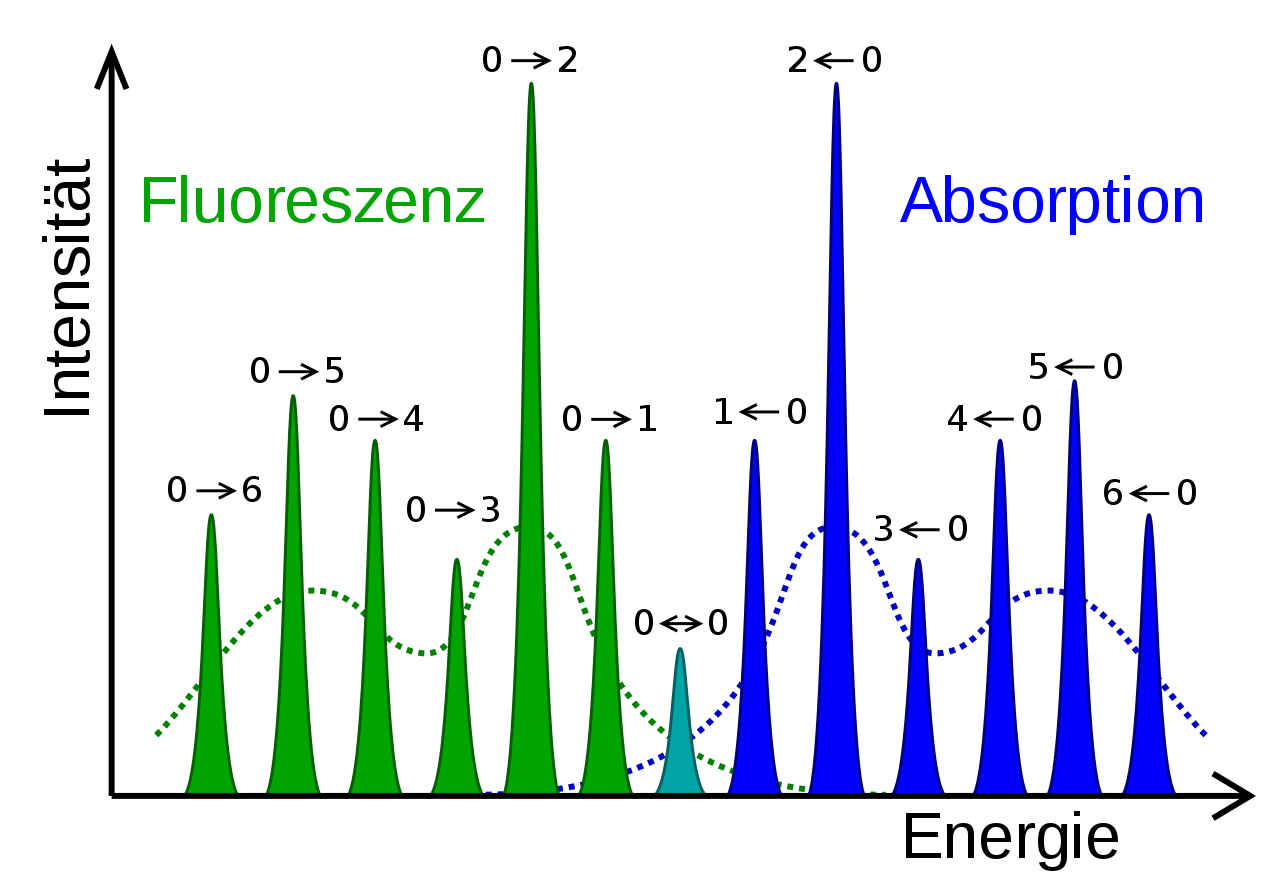
\includegraphics[width=\linewidth]{img/1280px-Franck-Condon-Prinzip_Intensitaeten.svg.png}}
    \subcaptionbox{Energie eines zweiatomigen Moleküls in Abhängigkeit vom theoretisch festgehaltenen Abstand der Kerne, für zwei verschiedene Zustände der Elektronenhülle (schematisch). Die Schwingungszustände sind mit ihren Wellenfunktionen für den Kernabstand auf der Höhe der jeweiligen Energie eingezeichnet. Die beiden Pfeile stellen vibronische Übergänge dar. \label{subfig:franck_condon:2}}[0.49\linewidth]{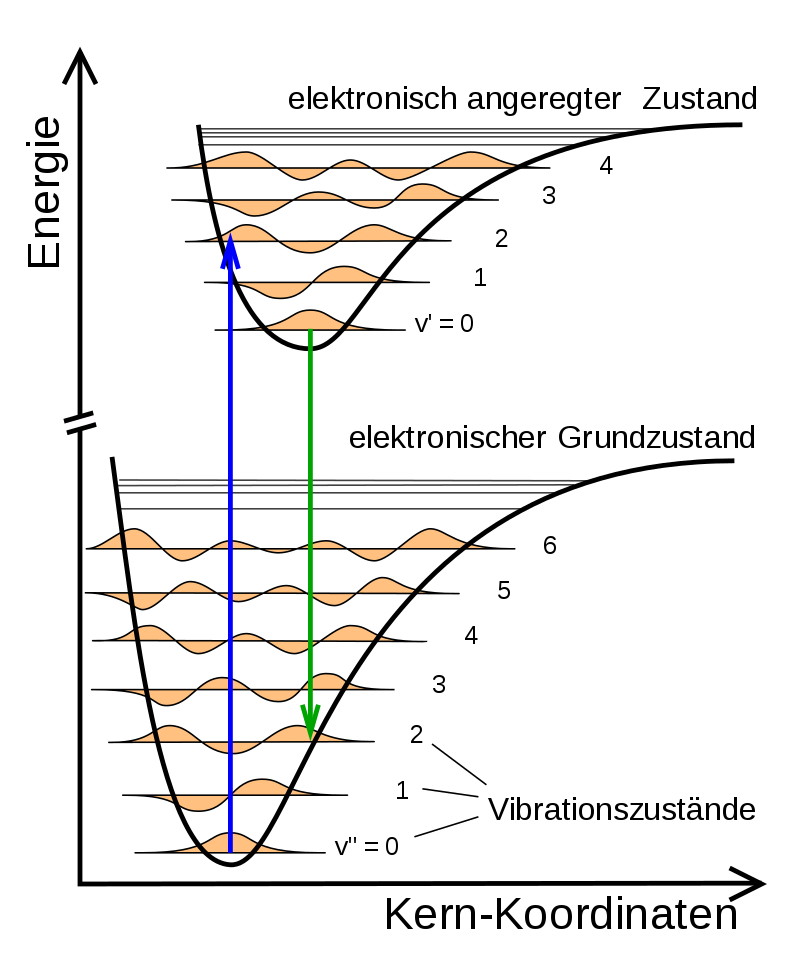
\includegraphics[width=\linewidth]{img/800px-Franck-Condon-Prinzip.svg.png}}
    \caption{Abbildungen zum Franck-Condon-Prinzip. \refimgsource{Wikimedia}{https://de.wikipedia.org/wiki/Franck-Condon-Prinzip}{23.02.2022}{public domain}}
    \label{fig:franck_condon}
\end{figure}

\begin{fquestion}{Was ist das Frank-Condon-Prinzip?}
    Das Frank-Condon-Prinzip beschreibt das Verhalten von Vibrationseigenzuständen eines Moleküls bei einer Änderung des Zustands des Elektrons (dem Übergang in eine andere Schale).
    Wegen seiner hohen Masse ist die Schwingungsperiode des Kerns mit $\approx \SI{e-13}{s}$ sehr viel länger als die Dauer eines elektrischen Übergangs $\approx \SI{e-15}{s}$; die Kernkonfiguration bleibt beim Übergang also starr (Born-Oppenheimer-Näherung).
    
    Dadurch geht der Vibrationszustand bevorzugt in einen anderer Quantenzahl, aber großer Überlappung über.
    Der neue Vibrationszustand ist dementsprechend nicht mehr der Vibrationsgrunzustand.
    Siehe \autoref{fig:franck_condon} für eine Illustration, besonders der blaue Pfeil für die Anregung.
\end{fquestion}

\begin{fquestion}{Wie steht das Frank-Condon-Prinzip mit dem Stokes-Shift im Zusammenhang?}
    Der Stokes-Shift beschreibt eine Verschiebung der Wellenlänge von Licht zwischen Absorption und Emission, etwa bei der Fluoreszenz:
    \begin{center}
        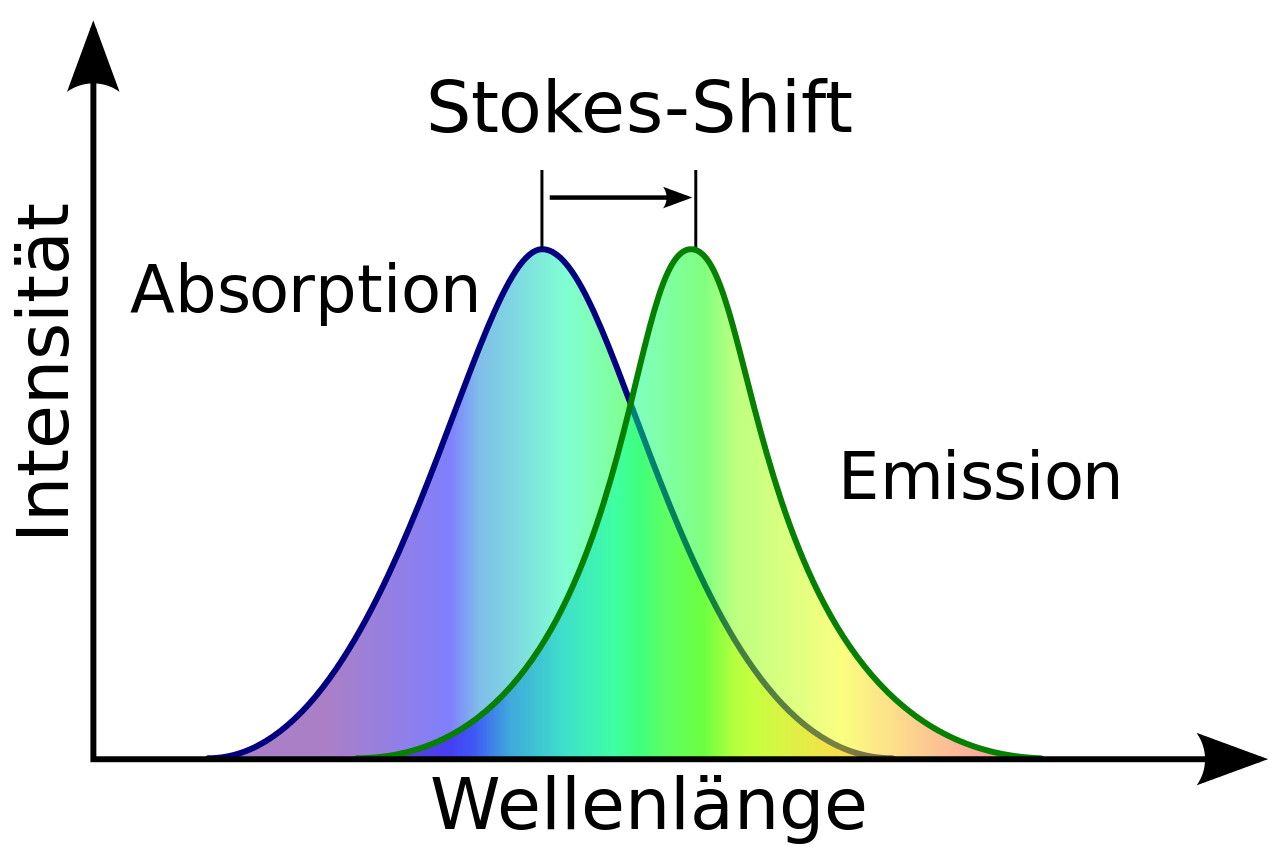
\includegraphics[width=0.4\linewidth]{img/1280px-Stokes-Verschiebung.svg.png}
    \end{center}
    Er entsteht dabei dadurch, dass ein Molekül nach der Anregung nicht mehr im vibratonischen Grundzustand ist (Franck-Condon-Prinzip).
    Die Abregung des vibratonischen Zustandes ist der elektronischen Abregung gegenüber bevorzugt, entsprechend findet zunächst die Abregung in den Grundzustand der Vibrationsmoden statt.
    Danach erfolgt erst die elektrische Abregung, welche entsprechend mit weniger Energie (höherer Wellenlänge) stattfindet.
    In \autoref{subfig:franck_condon:2} ist dies durch den blauen Pfeil für die elektrische Anregung in den grünen Pfeil für die elektrische Abregung dargestellt.
\end{fquestion}

% \begin{question}{Wie kommt die Bindung zustande?}
%     LCAO (Linear combination of atomic orbitals)
%     kovalente Bindung ???
% \end{question}

% \begin{question}{Ist das immer so?}
%     nein, kommt auf das Potential an
% \end{question}

\begin{fquestion}{Wenn man den antibindenden Zustand im Wasserstoff-Molekül zu Helium zusammenschiebt, was hat man dann?}
    Der antibindende Wasserstoffzustand hat näherungsweise die Form eines Heliums ${}_{2}\text{H}^+$ im $2p$-Zustand:
    \begin{center}
        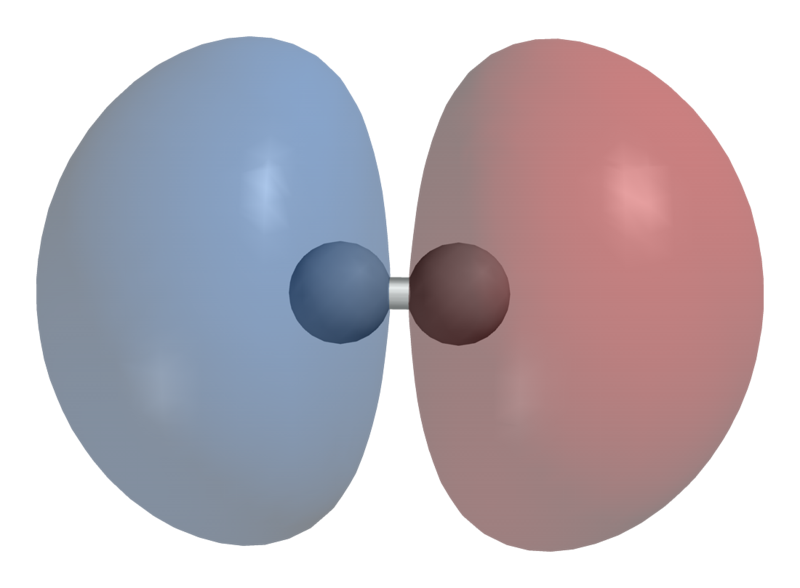
\includegraphics[width=0.3\linewidth]{img/800px-Dihydrogen-LUMO-phase-3D-balls.png}
    \end{center}
    \refimgsource{Wikimedia}{https://commons.wikimedia.org/wiki/File:Dihydrogen-LUMO-phase-3D-balls.png}{22.02.2022}{public domain}
\end{fquestion}

% \begin{question}{Spaltet der Grundzustand symmetrisch auf oder nicht bzgl der Energie?}
%     eigentlich ja, aber wegen der Absenkung der kinetischen Energie nicht ganz
% \end{question}

\begin{fquestion}{Wie sieht die Wellenfunktion eines Moleküls asymptotisch aus?}
    % Wie gewohnt exponentiell, übliches Verhalten für $\frac{1}{r^n}$-Potentiale.
    Exponentiell, wie für gebundene Zustände allgemein üblich.
\end{fquestion}

% \begin{question}{Beim Yukawa-Potential des Deuterons war die Pion-Masse relevant. Welche hier?}
%     Elektron für Bindung verantwortlich, also die Elektronenmasse.
% \end{question}

\subsection{Umrechnungen}

$\hbar c \simeq \SI{200}{MeV\,fm}$, $\SI{1}{meV} \simeq \SI{12}{K} \simeq \SI{8.4}{cm^{-1}}$ (Achtung: lineare Wellenzahl, siehe \autoref{fig:harmonic wave properties conversion}).
\\
Energie in Frequenz: $\SI{1}{eV} = \frac{e}{h} = f = \SI{242}{THz}$ (Achtung: $f\neq \omega = 2\pi f$).

\begin{figure}[!ht]
    \centering
    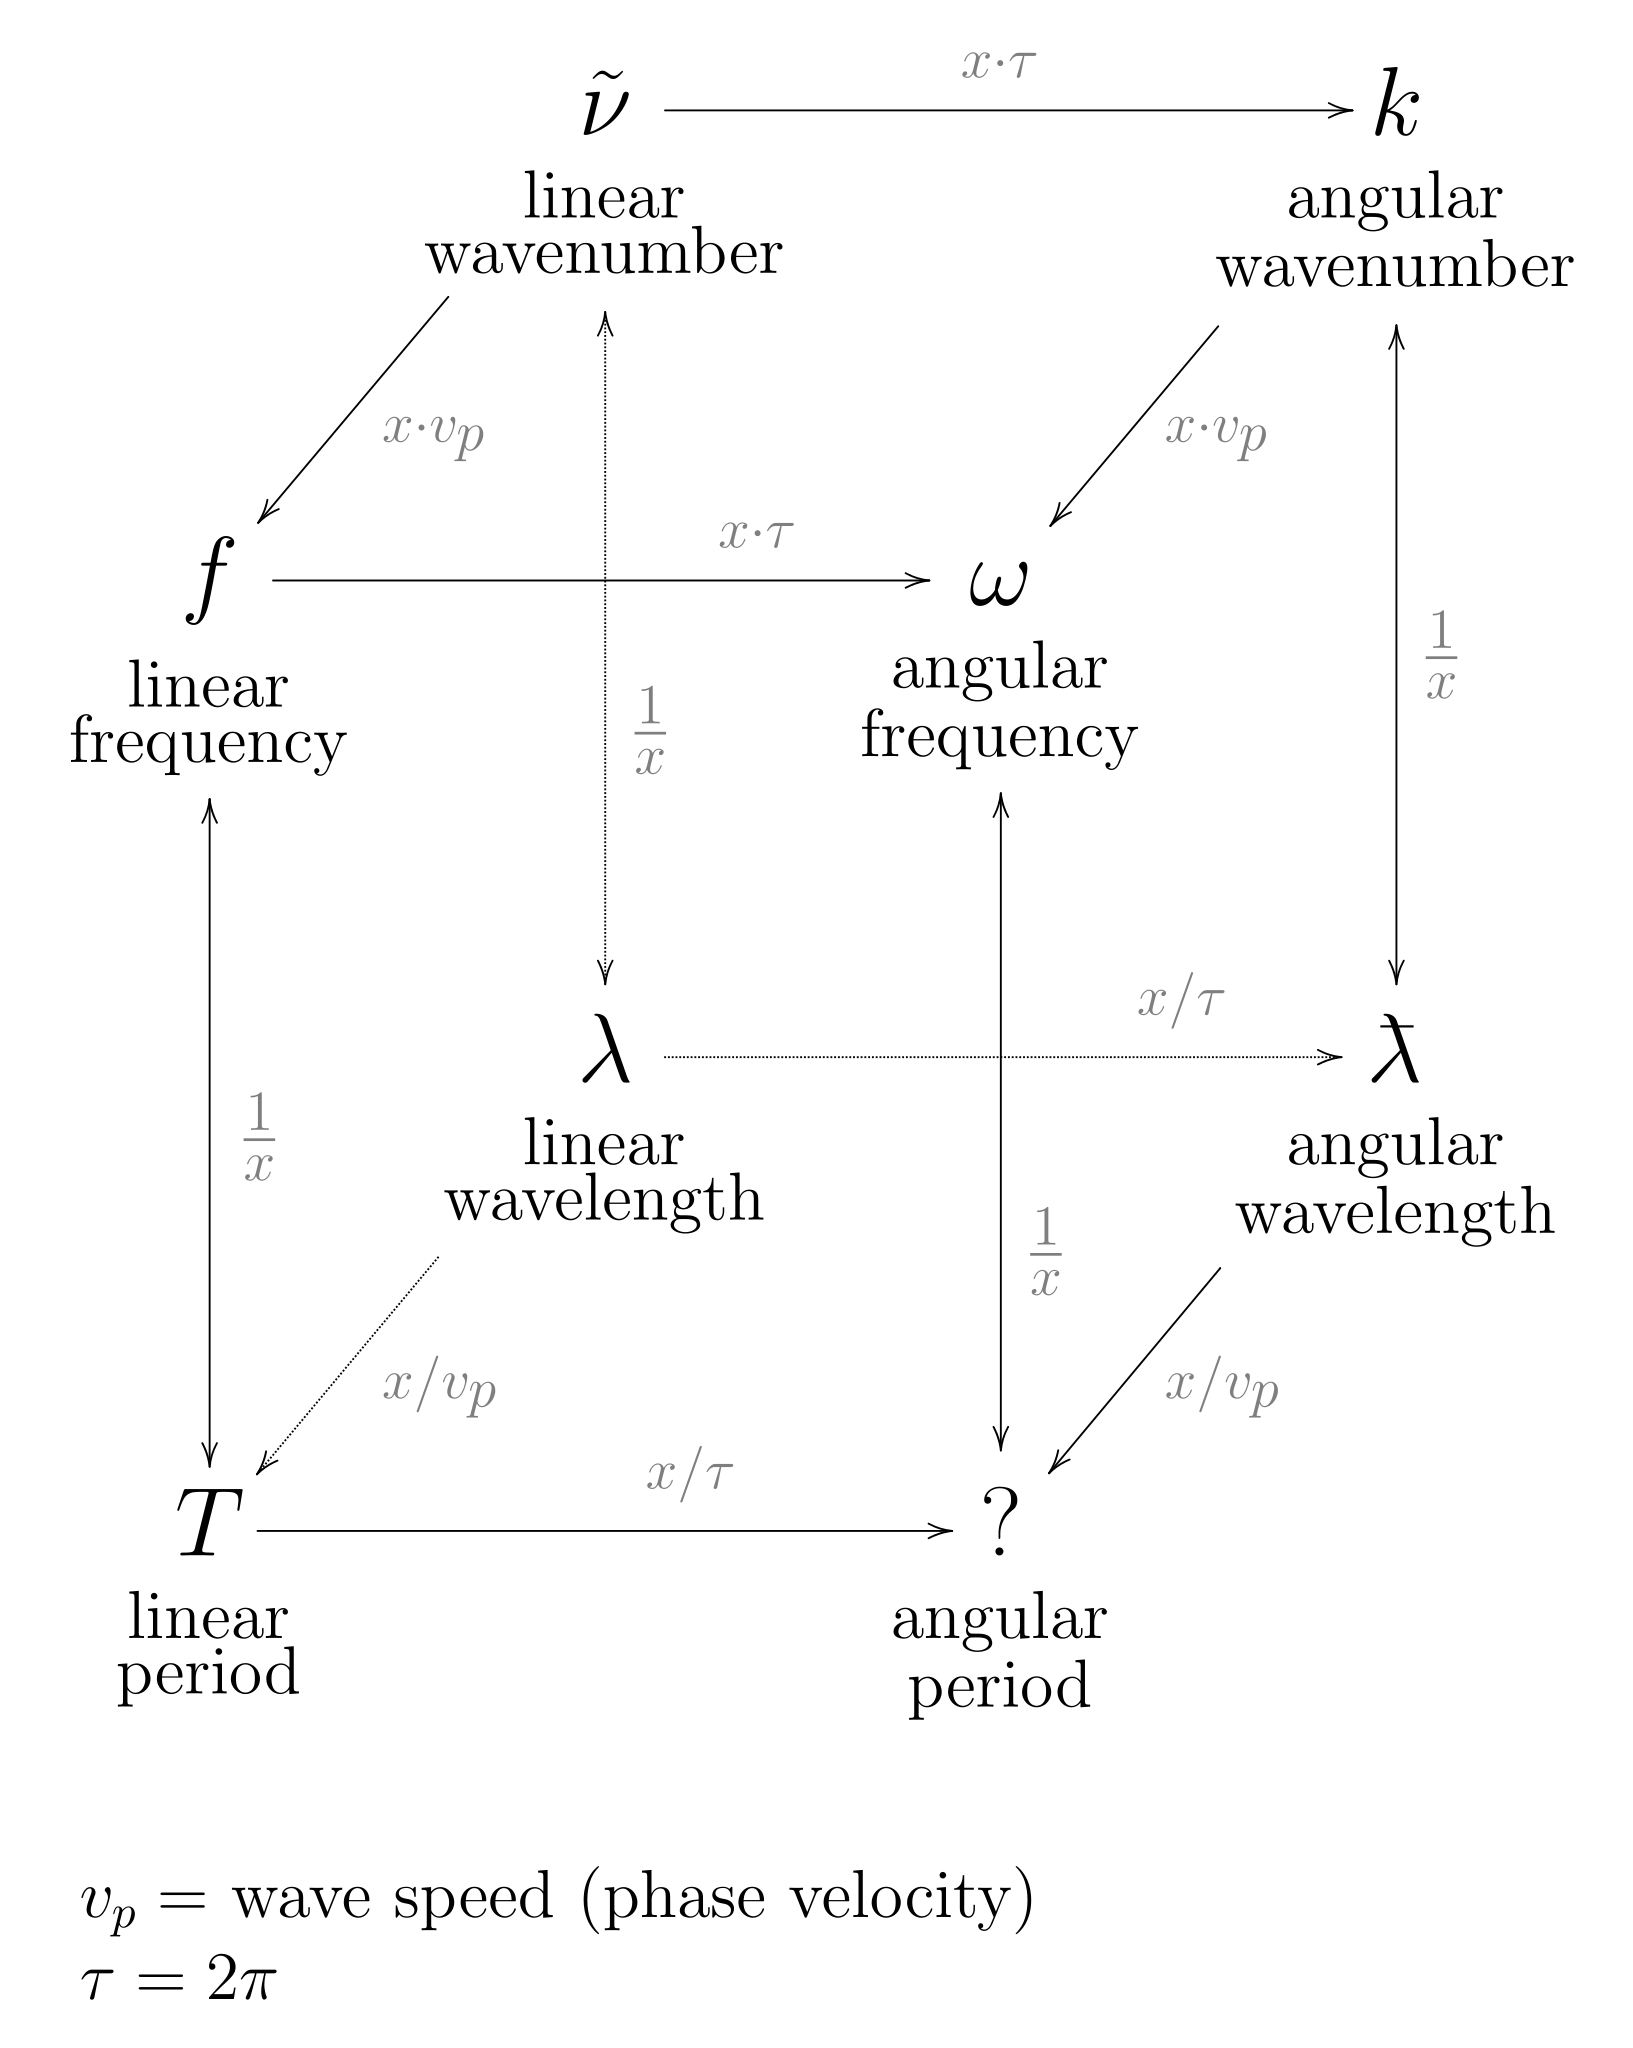
\includegraphics[width=.8\linewidth]{img/Commutative_diagram_of_harmonic_wave_properties.png}
    \caption{Grafische Darstellung der verschiedenen Eigenschaften einer Welle mit entsprechenden Konvertierungen.
    \refimgsource{Wikimedia}{https://commons.wikimedia.org/wiki/File:Commutative\_diagram\_of\_harmonic\_wave\_properties.svg}{24.02.2022}{public domain}}
    \label{fig:harmonic wave properties conversion}
\end{figure}






\begin{thebibliography}{9}
    \bibitem{Bur2000} Burkel, Eberhard. (2000). Phonon spectroscopy by inelastic x-ray scattering. Reports on Progress in Physics - REP PROGR PHYS. 63. 171-232. 10.1088/0034-4885/63/2/203. 
    % \bibitem{GhaGhaGha2012} Ghahramany, N., Gharaati, S. and Ghanaatian, M. New approach to nuclear binding energy in integrated nuclear model. J Theor Appl Phys 6, 3 (2012). \url{https://doi.org/10.1186/2251-7235-6-3}
    \bibitem{WanAudKonHuaNaiXu2016} Meng Wang, G. Audi, F. G. Kondev, W. J. Huang, S. Naimi and Xing Xu. The AME2016 atomic mass evaluation (II). Tables, graphs and references[J]. Chinese Physics C, 2017, 41(3): 030003.
    
\end{thebibliography}

\end{document}
